% Complete documentation on the extended LaTeX markup used for Python
% documentation is available in ``Documenting Python'', which is part
% of the standard documentation for Python.  It may be found online
% at:
%
%     http://www.python.org/doc/current/doc/doc.html

\documentclass[letterpaper,hyperref,titlepage]{manual}

% latex2html doesn't know [T1]{fontenc}, so we cannot use that:(

\usepackage{amsmath}
\usepackage{amssymb} 	% We need this for blacktriangleright and blacktriangleleft.
\usepackage[latin1]{inputenc}
\usepackage{textcomp}
\usepackage{fullpage}
\usepackage{graphicx}
\graphicspath{{./graphics/}}
\usepackage{url}
\usepackage{index}
\usepackage{chicago}
\usepackage{xtab}
\usepackage{multirow}
%\setlongtables
%\usepackage{epsfig}

% The commands of this document do not reset module names at section level
% (nor at chapter level).
% --> You have to do that manually when a new module starts!
%     (use \py@reset)
%begin{latexonly}
\makeatletter
\renewcommand{\section}{\@startsection{section}{1}{\z@}%
   {-3.5ex \@plus -1ex \@minus -.2ex}%
   {2.3ex \@plus.2ex}%
   {\reset@font\Large\py@HeaderFamily}}
\makeatother
%end{latexonly}

% additional mathematical functions
\DeclareMathOperator{\abs}{abs}

%%%
%%% Start of preamble ``borrowed'' from a Fernando Perez post tn the
%%% NumPy listserv on 02/11/06.
%%%

% This gives us a better font in URL links (otherwise the default
% MonoSpace font is bitmapped, and it looks horrible in PDF)
\usepackage{courier}
\usepackage{fullpage}
\usepackage{color}  % so we can use red for the fixme warnings

% The hyperref package gives us a pdf with properly built
% internal navigation ('pdf bookmarks' for the table of contents,
% internal cross-reference links, web links for URLs, etc.)

% A few colors to replace the defaults for certain link types
\definecolor{darkorange}{rgb}{.71,0.21,0.01}
\definecolor{darkgreen}{rgb}{.12,.54,.11}

\usepackage[
  %pdftex,  % needed for pdflatex
  breaklinks=true,  % so long urls are correctly broken across lines
  colorlinks=true,
  urlcolor=blue,
  linkcolor=darkorange,
  citecolor=darkgreen,
  ]{hyperref}

% This helps prevent overly long lines that stretch beyond the margins
\sloppy

% Define a \fixme command to mark visually things needing fixing in the draft.
% For final printing or to simply disable these bright warnings, simply
% uncomment the \renewcommand redefinition below

\newcommand{\fixme}[1] {
\textcolor{red}{
{\fbox{ {\bf FIX}
\ensuremath{\blacktriangleright \blacktriangleright \blacktriangleright}}
{\bf #1}
\fbox{\ensuremath{ \blacktriangleleft \blacktriangleleft \blacktriangleleft }
} } }
}
% Uncomment the next line to make the \fixme command be a no-op
%\renewcommand{\fixme}[1]{}

%%% If you also want to use the listings package for nicely formatted
%%% Python source code, this configuration produces good on-paper and
%%% on-screen results:

\definecolor{orange}{cmyk}{0,0.4,0.8,0.2}
% Use and configure listings package for nicely formatted code
\usepackage{listings}
\lstset{
  language=Python,
  basicstyle=\small\ttfamily,
  commentstyle=\ttfamily\color{blue},
  stringstyle=\ttfamily\color{orange},
  showstringspaces=false,
  breaklines=true,
  postbreak = \space\dots
}

%%%
%%% End of preamble ``borrowed'' from a Fernando Perez post tn the
%%% NumPy listserv on 02/11/06.
%%%

% some convenience declarations
\newcommand{\pypedal}{PyPedal}
\newcommand{\PyPedal}{PyPedal}  % Only beginning of sentence, otherwise use \pypedal{}
\newcommand{\PYPEDAL}{PyPedal}
\newcommand{\python}{Python}

% mark internal comments
% for any published version switch to the second (empty) definition of the macro!
% \newcommand{\remark}[1]{(\textbf{Note to authors: #1})}
\newcommand{\remark}[1]{}

\title{A Manual for use of PyPedal\\A software package for pedigree analysis}
\author{John B. Cole}
\authoraddress{Animal Improvement Programs Laboratory, Agricultural Research Service, United States Department of Agriculture, Room 306 Bldg 005 BARC-West, 10300 Baltimore Avenue, Beltsville, MD 20705-2350}

% I use date to indicate the manual-updates,
% release below gives the matching software version.
%\date{December 01, 2005}        % update before release!
\date{November 29, 2005 \\ Revised \today}                   % update before release!
                                % Use an explicit date so that reformatting
                                % doesn't cause a new date to be used.  Setting
                                % the date to \today can be used during draft
                                % stages to make it easier to handle versions.

\release{2.0.4}                 % (software) release version;
\setshortversion{2.0}           % this is used to define the \version macro
\makeindex                      % tell \index to actually write the .idx file
\newindex{func}{fdx}{fnd}{Function Index}

\begin{document}

\maketitle

\begin{abstract}
Cole, J.B.  2012.  A Manual for use of PyPedal: A software package for pedigree analysis.  Animal Improvement Programs Laboratory, Agricultural Research Service, United States Department of Agriculture.

This manual in twelve chapters describes PyPedal (v 2.0), a software package for pedigree analysis, report generation, and data visualization.  Metrics include coefficients of inbreeding and relationship, effective founder and ancestor numbers, and founder genome equivalents.  Tools are provided for identifying ancestors and descendants, computing coefficients of inbreeding from potential matings, quantifying pedigree completeness, and visualizing pedigrees.  Scripting support is provided by the Python programming language; this language may be used to easily automate analyses and implement new features. Input and output files utilize plain-text formats.  The program has been used for the analysis of dairy cattle and working dog pedigrees.  PyPedal runs on the GNU/Linux and Microsoft Windows operating systems.  The program, documentation, and examples of usage are available at \url{http://pypedal.sourceforge.net/}.

Mention of trade names or commercial products in this manual is solely for the purpose of providing specific information and does not imply recommendation or endorsement by the U.S. Department of Agriculture.

All programs and services of the U.S. Department of Agriculture are offered on a nondiscriminatory basis without regard to race, color, national origin, religion, sex, age, marital status, or handicap.

Revised \today
\end{abstract}

% This makes the contents more accessible from the front page of the HTML.
\ifhtml
\part*{General}
\chapter*{Front Matter}
\label{front}
\fi

\section*{Legal Notice}
\begin{quote}
 The only people who have anything to fear from free software are those whose products are worth even less. --- David Emery
\end{quote}

\label{sec:legal-notice}
Copyright (c) 2002-2012.  John B. Cole.  All rights reserved.

Permission to use, copy, modify, and distribute this software for any purpose
without fee is hereby granted, provided that this entire notice is included in
all copies of any software which is or includes a copy or modification of this
software and in all copies of the supporting documentation for such software.

\subsection*{Disclaimer}
The author of this software does not make any warranty, express or implied, or
assume any liability or responsibility for the accuracy, completeness, or
usefulness of any information, apparatus, product, or process disclosed, or
represent that its use would not infringe privately-owned rights. Reference
herein to any specific commercial products, process, or service by trade name,
trademark, manufacturer, or otherwise, does not necessarily constitute or imply
its endorsement, recommendation, or favoring by the United States Government or
the author. The views and opinions of authors expressed herein do not necessarily
state or reflect those of the United States Government and shall not be used for
advertising or product endorsement purposes.

\section*{License}\label{sec:license}\index{license}
This is free software; you can redistribute it and/or modify it
under the terms of the GNU Lesser General Public License as published by
the Free Software Foundation; either version 2.1 of the License, or (at
your option) any later version.

This software is distributed in the hope that it will be useful, but
WITHOUT ANY WARRANTY; without even the implied warranty of
MERCHANTABILITY or FITNESS FOR A PARTICULAR PURPOSE.  See the GNU
Lesser General Public License for more details.

You should have received a copy of the GNU Lesser General Public
License along with this library; if not, write to the Free Software
Foundation, Inc., 51 Franklin St, Fifth Floor, Boston, MA 02110-1301,
USA.

\tableofcontents
\listoftables
\listoffigures

\declaremodule{extension}{pypedal}
\moduleauthor{John B. Cole}{john.cole@ars.usda.gov}
\modulesynopsis{Py{P}edal}
\chapter{Introduction}
\label{cha:introduction}

\begin{quote}
Any sufficiently disguised bug is indistinguishable from a feature. --- Rich Kulawiec
\end{quote}
This chapter introduces the \PyPedal{} module for Python 2.4, provides an overview of key features of the software, and describes the contents of this manual.

\PyPedal{} (\textbf{P}ython \textbf{Ped}igree An\textbf{al}ysis) is a tool for analyzing pedigree files.  It calculates several quantitative measures of genetic diversity from pedigrees, including average coefficients of inbreeding and relationship, effective founder numbers, and effective ancestor numbers.  Checks are performed catch common mistakes in pedigree files, such as parents with more recent birthdates or smaller ID numbers than their offspring and animals appearing as both sires and dams in the pedigree.  Tools for pedigree visualization and report generation are also provided.  \PyPedal{} only makes use of information on pedigree structure, not individual genotypes.  Allelotypes can be assigned to founders for use in gene-dropping simulations to calculate the effective number of founder genomes, but no other measures of alleic diversity are currently supported.

\PyPedal{} is a Python (\url{http://www.python.org/}) language module that may be called by programs or used interactively from the interpreter.  You must have Python 2.7 (or later) installed in order to use \PyPedal{} as \PyPedal{} makes use of features found only in that version.  The Numarray module must also be installed in order for you to use \PyPedal{}, and may be found at \url{http://www.stsci.edu/resources/software_hardware/numarray}.  In addition, there are a number of third-party packages used by \PyPedal{}; they are discussed in Chapter \ref{cha:installation}.

This manual is the official documentation for \PyPedal{}. It includes a tutorial and is the most authoritative source of information about \PyPedal{} with the exception of the source code. The tutorial material will walk you through a set of manipulations of a simple pedigree.  All users of \PyPedal{} are encouraged to follow the tutorial with a working \PyPedal{} installation. The best way to learn is by doing --- the aim of this tutorial is to guide you along this doing.

This content of this manual is broken down as follows:
\begin{description}
\item[License] Chapter \ref{cha:license} describes the license under which \PyPedal{} is distributed.  It is important that you review the license before using the program.
\item[Installing PyPedal] Chapter \ref{cha:installation} provides information
   on testing Python and installing PyPedal.
\item[High-Level Overview] Chapter \ref{cha:high-level-overview} gives a
   high-level overview of the components of the \PyPedal{} system as a whole.
\item[Methodology] Chapter \ref{cha:methodology} provides a brief overview of the methodology used to calculate measures of genetic diversity.
\item[HOWTOs] Chapter \ref{cha:howtos} provides demonstrations of how to perform common tasks.
\item[Graphics] Chapter \ref{cha:graphics} provides details on producing graphics with \PyPedal{}.
\item[Reports] Chapter \ref{cha:reports} provides details about the report generation tools available in \PyPedal{}.
\item[Implementing New Features] Chapter \ref{cha:newfeatures} introduces the idea of extensibility and walks the reader through the development of a new \PyPedal{} routine.
\item[Applications Programming Interface] Chapter \ref{cha:api} includes a complete reference, including useage notes, for all functions in all \PyPedal{} modules.
% \item[PyPedal Tutorial] Chapter \ref{cha:tutorial} provides brief tutorial for new users of \PyPedal{}.
\item[Glossary] Chapter \ref{cha:glossary} provides a glossary of terms.
\item[References and Indices] are provided at the end of the manual.
\end{description}

\section{Features}
Some of the notable features of \PyPedal{} include:
\begin{itemize}
\item Reading pedigree files in user-defined formats;
\item Checking pedigree integrity (duplicate IDs, parents younger than offspring, etc.);
\item Generating summary information such as frequency of appearance in the pedigree file;
\item Reordering and renumbering of pedigree files, including those with IDs as character strings rather than integers;
\item Computation of the numerator relationship matrix ($A$) from a pedigree file using the tabular method;
\item Inbreeding and relationship calculations for large pedigrees (pedigrees up to 600,000 animals have been processed with \PyPedal{});
\item Computation of coefficients of inbreeding using the Meuwissen and Luo \cite{ref585} and modified Meuwissen and Luo (Quaas, 1993) algorithms;
\item Computation of average total and individual coefficients of inbreeding and relationship;
\item Calculation of coefficients of partial inbreeding using an iterative tabular method \cite{LacyAW1996,GulisijaGWT2006};
\item Calculation of coefficients of ancestral inbreeding using the methods of Ballou \citeyear{Ballou1997} or Suwanlee et al. \citeyear{SuwanleeBSC2007};
\item Decomposition of $A$ into $T$ and $D$ such that $A=TDT'$;
\item Computation of the direct inverse of $A$ (not accounting for inbreeding) using the method of Henderson \citeyear{ref143};
\item Computation of the direct inverse of $A$ (accounting for inbreeding) using the method of Quaas \citeyear{ref235};
\item Storage of $A$ and its inverse between user sessions as persistent Python objects using the \textbf{pickle} module to avoid unnecessary calculations;
\item Calculation of theoretical and actual effective population sizes;
\item Computation of effective founder number using the exact algorithm of Lacy \citeyear{ref640};
\item Computation of effective founder number using the approximate algorithm of Boichard et al. \citeyear{ref352};
\item Computation of effective ancestor number using the algorithms of Boichard et al. \citeyear{ref352};
\item Selection of subpedigrees containing all ancestors of an animal;
\item Identification of the common relatives of two animals;
\item Calculation of the inbreeding of offspring from a prospective mating;
\item Output to ASCII text files, including matrices, coefficients of inbreeding and relationship, and summary information;
\item Importation and exportation of GEDCOM 5.5 files;
\item Importation and exportation of GENES 1.20 (dBase III) files;
\item Loading pedigrees from, and saving them to, MySQL, Postgres, and SQLite databases;
\item Simulation of pedigrees using an algorithm derived from that in Matvec 1.1a;
\item Set operations on pedigrees (unions and intersections);
\end{itemize}
\PyPedal{} has been used to perform calculations on pedigrees as large as 600,000 animals and has been used in scientific research \cite{Cole2004a,Cole2007a}.

\section{Where to get information and code}
\PyPedal{} and its documentation are available at: \url{http://pypedal.sourceforge.net/}.  The Sourceforge site, \url{http://sourceforge.net/projects/pypedal/}, provides tools for reporting bugs (\url{https://sourceforge.net/tracker/?func=add&group_id=106679&atid=645233}, making feature requests (\url{https://sourceforge.net/tracker/?func=add&group_id=106679&atid=645236}), and discussing \PyPedal{} (\url{https://sourceforge.net/forum/?group_id=106679}). The current development code can be downloaded from the \PyPedal{} git repository at \url{https://github.com/wintermind/pypedal}.

\section{Acknowledgments}\index{Acknowledgments}
\PyPedal{} was initially written to support the author's dissertation research while at Louisiana State University, Baton Rouge (\url{http://www.lsu.edu/}).  The initial development was supported in part by a grant from The Seeing Eye, Inc., Morristown, NJ, USA.  It lay fallow for some time but has recently come under active development again.  This is due in part to a request from colleagues at the University of Minnesota that led to the inclusion of new functionality in \PyPedal{}.  The author wishes to thank Paul Van{R}aden for very helpful suggestions for improving the ability of \PyPedal{} to handle certain computations in large pedigrees.  Additional feedback in the form of bug reports, feature requests, and discussion of computing strategies was provided by Dan Cieslak, Bradley J. Heins (University of Minnesota-Twin Cities), Edward H. Hagen (Institute for Theoretical Biology, Humboldt-Universit\"{a}t zu Berlin), Kathy Hanford (University of Nebraska, Lincoln), Thomas Kelly (Department of Animal and Poultry Science, University of Guelph), Thomas von Hassell, Gianluca Saba, and Ken Severin (University of Alaska -- Fairbanks). Gregor Gorjanc has written a blog entry describing \href{http://ggorjan.blogspot.com/2007/04/installing-pypedal-under-debian.html}{how to install PyPedal on Debian Linux}. Fernando Perez posted a \LaTeX preamble to the NumPy listserver that dramatically improved the PDF version of This Manual.

The Newfoundland pedigree presented in Figure \ref{fig:newfoundland-colored-pedigree} was taken from the NewFoundland Dog database (\url{http://www.newfoundlanddog-database.net/en/}) and is used with permission.

The pedigree of European royalty used in the GEDCOM discussion (Appendix \ref{GEDCOM}), \href{http://www.genealogyforum.com/gedcom/gedcom1/ged3.htm}{ged3.ged}, was taken from the Genealogy Forum website (\url{http://www.genealogyforum.com/}). It is believed to be in the public domain, and is used with the knowledge of the website administrators.

\section{Disclaimer}\index{Disclaimer}
Reference to any commercial product is made with the understanding that no discrimination is intended and no endorsement by USDA is implied.

\chapter{Installing PyPedal}\label{cha:installation}\index{installation}
\begin{quote}
As we acquire more knowledge, things do not become more comprehensible, but more mysterious. --- Will Durant
\end{quote}
This chapter explains how to install and test \PyPedal{} under Posix-type operating systems and Microsoft Windows.

\section{Overview of installation}\label{sec:installation-overview}
Before we can begin the tutorial, you need install and test Python, NumPy and some other Python extensions, and \PyPedal{} itself. \PyPedal{} has been tested against the versions listed in Table \ref{tbl:extensions}, and may not work with earlier releases of those packages. The extensions that you need to install in order to use all of the features of \PyPedal{} are listed in Table \ref{tbl:extensions}.  Note that some extensions need to be installed before others: \module{Numpy} should be installed first, and \module{pyparsing} and Graphviz must be installed before \module{pydot}.

If you do not install one or more optional modules you will still be able to use \PyPedal{}, although some features may not be available to you. Details on installing the extensions listed above can be found on their respective websites.  All of these extensions are available for Unix-type operating systems (e.g. Linux, Mac OS X) as well as for Microsoft Windows; most sites also provide binary installers for Windows. Python extensions can usually be installed by unzipping/untaring the archives, entering the folder, and issuing the command \samp{python setup.py install} as a root/administrative user. Note that NetworkX and ReportLab are not installed by the Enthought Python Distribution for Windows. I have found that installations from source on Linux are sometimes tricky, but I have found that Sage (\url{http://www.sagemath.org/index.html}) does a great job of getting clean builds of the trickier pieces, such as Numpy and matplotlib.
\begin{center}
    \tablecaption{Packages and compatible versions used by \PyPedal{}.}
    \tablefirsthead{\hline Extension & Version & Used for... & URL \\ \hline}
    \tablehead{\hline Extension & Version & Used for... & URL \\ \hline}
    \tabletail{\hline \multicolumn{4}{l}{\small\sl continued on next page} \\ \hline}
    \tablelasttail{\hline}
    \label{tbl:extensions}
    \index{installation!extensions}
    \begin{xtabular}{lllp{4in}}
	elementtree &  & Lightweight XML processing & \url{http://effbot.org/zone/element-index.htm}\\
	Graphviz &  & Draw directed graphs & \url{http://www.research.att.com/sw/tools/graphviz/}\\
	matplotlib &  & Plotting, matrix visualization & \url{http://matplotlib.sourceforge.net/}\\
	NetworkX &  & Network analysis & \url{https://networkx.lanl.gov/}\\
	Numpy &  & Array manipulation & \url{http://www.numpy.org/}\\
	PIL &  & Image processing & \url{http://effbot.org/zone/pil-index.htm}\\
	pydot &  & Interface to Graphviz & \url{http://dkbza.org/pydot.html}\\
	PyGraphviz &  & Interface to Graphviz & \url{https://networkx.lanl.gov/wiki/pygraphviz}\\
	pyparsing &  & Text parsing & \url{http://pyparsing.sourceforge.net/}\\
	Python &  & Pretty much everything & \url{http://python.org/}\\
	ReportLab &  & Generate PDF documents & \url{http://www.reportlab.org/}\\
	testoob &  & Advanced unit testing & \url{http://testoob.sourceforge.net/}\\
    \end{xtabular}
\end{center}
The \PyPedal{} distribution includes a copy of the ADOdb for Python (\url{http://http://phplens.com/lens/adodb/adodb-py-docs.htm/}) database abstraction library. It is installed with \PyPedal{} and does not require a separate installation step.

\section{Testing the Python installation}
The first step is to install Python 2.4 (or later) if you haven't already done so. Python is available at
\url{http://sourceforge.net/projects/python/}.  Click on the link corresponding to your platform, and follow the instructions presented there. Python can usually be started by typing \samp{python} at the shell (Posix) or double-clicking on the Python interpreter (Windows).  When you start Python you should see a message like:
\begin{verbatim}
Python 2.5.2 (r252:60911, Apr  8 2008, 21:49:41)
[GCC 4.2.3 (Ubuntu 4.2.3-2ubuntu7)] on linux2
Type "help", "copyright", "credits" or "license" for more information.
\end{verbatim}
If you have problems getting Python to work, contact your local support person or e-mail  \ulink{python-help@python.org}{mailto:python-help@python.org} for help.

\section{Installing PyPedal}\label{sec:installing-pypedal}
In order to get \PyPedal{}, visit the official website at \url{http://pypedal.sourceforge.net/}. Click on the "Sourceforge Page" link, click on the "Download PyPedal" button, and select the latest file release. Files whose names end in ``.tar.gz'' or ``.zip''are source code releases. The \PyPedal{} installation will not fail if a prerequisite package is not present, but not all \PyPedal{} functionality will be available to you.

\subsection{Installing on Unix, Linux, and Mac OSX}\label{sec:installing-unix}\index{installation!installation on Linux}
The source distribution should be uncompressed and unpacked as follows (for example):
\begin{verbatim}
gunzip pypedal-2.0.0rc4.tar.gz
tar xf pypedal-2.0.0rc4.tar.gz
\end{verbatim}
Follow the instructions in the top-level directory for compilation and installation. Installation is usually as simple as:
\begin{verbatim}
python setup.py install
\end{verbatim}
\paragraph*{Important Tip} \label{sec:tip:from-pypedal-import} Just like all Python modules and packages, the \PyPedal{} module can be invoked using either the \samp{import PyPedal} form, or the \samp{from PyPedal import ...} form.  All of the code samples will assume that they have been preceded by statements such as:
\begin{verbatim}
>>> from PyPedal import <module-name>
\end{verbatim}
A complete list of modules is provided in Chapter \ref{cha:api}.

\subsection{Installing on Windows}\label{sec:installing-windows}\index{installation!installation on Windows}
To install \PyPedal{}, you need to be logged into an account with Administrator privileges.  As a general rule, always remove any old version of \PyPedal{} before installing the current version.

Please note that \PyPedal{} has been lightly-tested on Windows XP, but I cannot guarantee that it runs without problems on Win-32 platforms!  \PyPedal{} should install and run properly on Win-32 as long as the dependencies listed above are satisfied. \index{installation!installation on Windows!Python Enthought Edition}Enthought provides a Python distribution that is bundled with a number of extras, including most of the dependencies needed to install and run \PyPedal{} in the Windows environment (\url{http://enthought.com/products/epd.php}). It is a large download (>100 MB) but greatly simplifies installation. If you use the Enthought distribution you will still need to download and install ReportLab (Table \ref{tbl:extensions}). Please note that the Enthought Python Distribution is free for academic and hobbyist use; if you intend to use it commercially (as part of your business) please pay the license fee or do not use their product. With the exception of \module{PyGraphviz}, which is discussed below, the prerequisite packages are available as Windows installation (.msi) files that can be downloaded and installed individually.

\fixme{There is not yet an easy way to install the \module{PyGraphviz}\index{PyGraphviz} library under Windows. \module{PyGraphviz} is used by some of the graphics routines for rendering pedigrees. Windows users will need to refer to Chapter \ref{cha:graphics} for details on routines which require this module.}

It is possible that the installation may fail with the message \begin{verbatim}error: Download error: (10060, 'Operation timed out')\end{verbatim}. This means that the installer was trying to download a dependency and that operation was unsuccessful. This can usually be remedied by simply running the installer again.

\index{installation!installation on Windows!environment variables}In order to get your installation working correctly you will need to set some environment variables.  Under Windows XP (and 2000) you access those variables by right-clicking on the \emph{My Computer} icon on your desktop, selecting \emph{Properties}, selecting the \emph{Advanced} tab, and clicking the \emph{Environment Variables} button. First, add \texttt{;C:\textbackslash{}Python24} to the \envvar{PATH} by selecting it in the \emph{System Variables} list and clicking \emph{Edit}. Next, create a \envvar{PYTHONPATH} environment variable by clicking the \texttt{New} button under \texttt{User Variables}, entering the path to the \PyPedal{} directory in the \texttt{Variable value} field.

\subsubsection{Installation from source}\label{sec:installation-from-source}\index{installation!installation from source}
\begin{enumerate}
\item Unpack the distribution using an unzipping utility such as 7-Zip (\url{http://www.7-zip.org/}) that understands gzipped-and-tarred files. Once you've done that, open a shell by left-clicking on "Start", selecting "Run", and typing \texttt{cmd} into the box. Navigate to the directory into which you unpacked the \PyPedal{} distributio(this is an example, your file location may vary):
\begin{verbatim}
C:\> cd C:\PyPedal
\end{verbatim}
\item Build it using the distutils defaults:
\begin{verbatim}
C:\PyPedal> python setup.py install
\end{verbatim}
This installs \PyPedal{} in \texttt{C:\textbackslash{}python24\textbackslash{}site-packages}.
\end{enumerate}

\subsubsection{Installation on Cygwin} \label{sec:installation-cygwin}\index{installation!installation on Cygwin}
No information on installing \PyPedal{} on Cygwin is available.  If you manage to get it working, please let me know.

\section{Testing the PyPedal Installation}\label{sec:installation-testing}\index{installation!testing the installation}
To find out if you have correctly installed \PyPedal{}, type \samp{import PyPedal} at the Python prompt. You'll see one of two behaviors (throughout this document user input and Python interpreter output will be emphasized
as shown in the block below):
\begin{verbatim}
>>> import PyPedal
Traceback (innermost last):
File "<stdin>", line 1, in ?
ImportError: No module named PyPedal
\end{verbatim}
indicating that you don't have \PyPedal{} installed, or:
\begin{verbatim}
>>> import PyPedal
>>> PyPedal.__version__.version
'2.0.0rc4'
\end{verbatim}
indicating that \PyPedal{} is installed.

\chapter{High-Level Overview}
\label{cha:high-level-overview}
\begin{quote}
By a small sample we may judge the whole piece. --- Miguel de Cervantes Saavedra
\end{quote}
\section{Interacting with PyPedal}
\label{sec:interacting}
\index{interacting with PyPedal}
There are two ways to interact with \PyPedal{}: interactively\index{interacting with PyPedal!interactively} from a Python command line, and programmatically\index{interacting with PyPedal!programmatically} using a script that is run using the Python interpreter.  The latter is preferred to the former for any but trivial examples, although it is useful to work with the command line while learning how to use \PyPedal{}.  A number of sample programs are included with the \PyPedal{} distribution. %Examples of both styles of interaction may be found in the tutorial (Chapter \ref{cha:tutorial}).
\section{The PyPedal Object Model}
\label{sec:pypedal-objects}
\index{objects}
At the heart of \PyPedal{} are four different types of objects.  These objects
combine data and the code that operate on those data into convenient packages.
Although most \PyPedal{} users will only work directly with one or two of these
objects it is worthwhile to know a little about each of them.  An instance of the
\class{NewPedigree} class stores a pedigree read from an input file, as well as
metadata about that pedigree.  The pedigree is a Python list of \class{NewAnimal}
objects.  Information about the pedigree, such as the number and identity of founders,
is contained in an instance of the \class{PedigreeMetadata} class.

The fourth \PyPedal{} class, \class{New{AM}atrix}, is used to manipulate numerator
relationship matrices (NRM).  When working with large pedigrees it can take a long
time to compute the elements of a NRM, and having an easy way to save and restore
them is quite convenient.

\PyPedal{} also provides \class{LightAnimal} and \class{SimAnimal} objects. \class{LightAnimal}s
are intended for use with the graph theoretic routines provided in \module{pyp_network} and lack
many of the attributes of \class{NewAnimal} objects, such as names, breeds, and alleleotypes.
\class{SimAnimal}s are intended for internal use only by the pedigree simulation routines.

A detailed explanation of each class is provided in Chapter \ref{cha:using-pypedal-objects}.
\section{Program Structure}
\label{sec:overview-program-structure}
\index{program structure}
\PyPedal{} programs load pedigrees from files and operate on those pedigrees.  A program consists of four basic parts: a header, an options section, pedigree creation, and pedigree operations.  The program header is used to import modules used in that program, and may include any Python module available on your system.  You must import a module before you can use it:
\begin{verbatim}
# Program header -- load modules used by a program
from PyPedal import pyp_newclasses
from PyPedal import  pyp_metrics
\end{verbatim}
You should only import modules that you are going to use in your program; you do not need to import every \PyPedal{} module in every program you write.

\PyPedal{} recognizes a number of different options that are used to control its behavior (Section \ref{sec:pypedal-options}).  Before you can load your pedigree into a \PyPedal{} object you must provide a pedigree file name (\samp{pedname}) and a pedigree format string (\samp{pedformat}).  This is done by either creating a Python dictionary and passing it as a parameter when \method{pyp_newclasses.loadPedigree()} is called or by specifying a configuration file\index{configuration file} name.  For example, here is how you would create and populate an options dictionary:
\begin{verbatim}
options = {}
options['messages'] = 'verbose'
options['renumber'] = 0
options['pedfile'] = 'new_lacy.ped'
options['pedformat'] = 'asd'
options['pedname'] = 'Lacy (1989) Pedigree'
\end{verbatim}
The syntax used in a configuration file is similar.  Consider the file \file{options.ini}, which contains the same options as set in the \var{options} dictionary in the previous example:
\begin{verbatim}
# options.ini
# This is an example of a PyPedal configuration file
messages = verbose
renumber = 0
pedfile = new_lacy.ped
pedformat = asd
pedname = Lacy (1989) Pedigree
\end{verbatim}
More details on configuration files are provided in Section \ref{sec:pypedal-options-file}.

You may name your dictionary or configuration file whatever you like; the examples in this manual, as well as those distributed with \PyPedal{}, use the name \samp{options}.  Once you have defined your options to is time to load your pedigree.  This is as simple as calling \function{pyp_newclasses.NewPedigree()}:
\begin{verbatim}
example = pyp_newclasses.loadPedigree(options)
\end{verbatim}
If you would like to use a configuration file to set your pedigree options, supply the configuration file name using the \var{optionsfile} keyword:
\begin{verbatim}
example = pyp_newclasses.loadPedigree(optionsfile='options.ini')
\end{verbatim}
Once you have loaded your pedigree file into a \class{NewPedigree} object you can unleash the awesome power of a fully-functional \PyPedal{} installation on it.  For example, calculating the effective number of founders in your pedigree using Lacy's \citeyear{ref640} exact method is as simple as:
\begin{verbatim}
pyp_metrics.effective_founders_lacy(example)
\end{verbatim}
Example programs that demonstrate how to use many of the features of \PyPedal{} are included in the \samp{examples} directory of the distribution.
\section{Options}
\label{sec:pypedal-options}
\index{options}
Many aspects of \PyPedal{}'s operation can be controlled using a series of options.  A complete list of these options, their defaults, and a brief description of their purpose is presented in Table \ref{tbl:options}.  Options are stored in a Python dictionary that you must create in your programs.  You must specify values for the \var{pedfile} and \var{pedformat} options; all others are optional.  \var{pedfile} is a string containing the name of the file from which your pedigree will be read.  \var{pedformat} is a string containing a pedigree format code (see section \ref{sec:pedigree-format-codes}) for each column in the datafile in the order in which those columns occur.  The following code fragment demonstrates how options are specified.
\begin{verbatim}
options = {}
options['messages'] = 'verbose'
options['renumber'] = 0
options['counter'] = 5
options['pedfile'] = 'new_lacy.ped'
options['pedformat'] = 'asd'
options['pedname'] = 'Lacy Pedigree'
example = pyp_newclasses.loadPedigree(options)
\end{verbatim}
First, a dictionary named \var{options} is created; you may use any name you like as long as it is a valid Python variable name.  Next, values are assigned to several options.  Finally, \var{options} is passed to \function{pyp\_newclasses.loadPedigree()}, which requires that you pass it either a dictionary of options or a configuration file name.  If you do not provide one of these, \PyPedal{} will halt with an error.

A single \PyPedal{} program may be used to read one or more pedigrees.  Each pedigree that you read must be passed its own dictionary of options.  The easiest way to do this is by creating a dictionary with global options.  You can then customize the dictionary for each pedigree you want to read.  Once you have created a \PyPedal{} pedigree by calling \function{pyp\_newclasses.NewPedigree(options)} you can change the options dictionary without affecting that pedigree because it has a separate copy of those options stored in its \member{kw} attribute.  The following code fragment demonstrates how to read two pedigree files using the same dictionary of options.
\begin{verbatim}
options = {}
options['messages'] = 'verbose'
options['renumber'] = 0
options['counter'] = 5

if __name__ == '__main__':
#   Read the first pedigree
    options['pedfile'] = 'new_lacy.ped'
    options['pedformat'] = 'asd'
    options['pedname'] = 'Lacy Pedigree'
    example1 = pyp_newclasses.loadPedigree(options)
#   Read the second pedigree
    options['pedfile'] = 'new_boichard.ped'
    options['pedformat'] = 'asdg'
    options['pedname'] = 'Boichard Pedigree'
    example2 = pyp_newclasses.loadPedigree(options)
\end{verbatim}
Note that \var{pedformat} only needs to be changed if the two pedigrees have different formats.  Only \var{pedfile} \emph{has} to be changed at all.

All pedigree options other than \var{pedfile} and \var{pedformat} have default values.  If you provide a value that is invalid the option will revert to the default.  In most cases, a message to that effect will also be placed in the log file.
\begin{center}
    \tablecaption{Options for controlling PyPedal.}
    \tablefirsthead{\hline Option & Default & Note(s) \\ \hline}
    \tablehead{\hline Option & Default & Note(s) \\ \hline}
    \tabletail{\hline \multicolumn{3}{l}{\small\sl continued on next page} \\ \hline}
    \tablelasttail{\hline}
    \label{tbl:options}
    \index{options!list}
    \begin{xtabular}{l|l|p{4in}}
	alleles\_sepchar  & '/'          & The character separating the two alleles in an animal's allelotype. \var{alleles\_sepchar} CANNOT be the same as \var{sepchar}! \\
	animal\_type  & 'new'            & Indicates which animal class should be used to instantiate animal records, \class{NewAnimal} or \class{LightAnimal} (`new'|`light'). \\
	counter          & 1000          & How often should \PyPedal{} write a note to the screen when reading large pedigree files. \\
	database\_debug  & False         & Toggle debugging messages in the database module on and off. \\
	database\_host   & 'localhost'   & The server on which the database is running. \\
	database\_name   & 'pypedal'     & The name of the database to be used. \\
	database\_passwd & 'anonymous'   & The password needed to connect to your database. \\
	database\_port   & ''            & The port on which your database is listening for connections (needed only for Postgres). \\
	database\_table  & 'filetag'     & The name of the database table to which the current pedigree will be written. \\
	database\_type   & 'sqlite'      & The type of database you are using ('mysql'|'postgres'|'sqlite'). \\
	database\_user   & 'anonymous'   & The name of a user with access rights to your database.  \\
	default\_fontsize & 10           & Specifies the default font size used in \module{pyp   \_graphics}. If the font size cannot be cast to an integer, it is set to the default value of 10. Font sizes less than 1 are set to the default of 10. \\
	default\_report   & filetag      & Default report name for use by \module{pyp\_reports}. \\
	default\_unit     & 'inch'       & The default unit of measurement for report generation ('cm'|'inch'). \\
	debug\_messages  & 0            & Indicates whether or not \PyPedal{} should print debugging information. \\
	f\_computed       & 0            & Indicates whether or not coefficients of inbreeding  have been computed for animals in the current pedigree.  If the pedigree format string includes \character{f} this will be set to 1; it is also set to 1 on a successful return from \function{pyp\_nrm/inbreeding()}. \\
	file\_io         & 1            & When true, routines that can write results to output files will do so and put messages in the program log to that effect. \\
	filetag          & pedfile      & \var{filetag} is a descriptive label attached to output files created when processing a pedigree.  By default the filetag is based on \var{pedfile}, minus its file extension. \\
	form\_nrm        & 0            & Indicates whether or not to form a NRM and bind it to the pedigree as an instance of a \class{NewAMatrix} object. \\
	foundercoi	 & 0		& Tells \function{pyp\_nrm.fast\_a\_matrix()} whether or not to use coefficients of inbreeding from the pedigree to augment the diagonals for founders.\\
	gen\_coeff       & 0            & When nonzero, calculate generation coefficients using the method of Pattie \citeyear{Pattie1965} and store them in the \member{gen\_coeff} attribute of a \class{NewAnimal} object.  The inferred generation stored in the \member{igen} attribute will be the \member{gen\_coeff} rounded to the nearest 0.5.  When zero, the \member{gen\_coeff} is -999. \\
	has\_header	 & 0		& When 1, the first row of the pedigree file is converted to a comment because it is a list of column names rather than data. If you are using a configuration file, you \emph{must} enclose the comma in double quotation marks (e.g., \code{has_header = ``,''}). \\
	log\_long\_filenames & 0        & When nonzero, long logfile names will be used, which means that log file names will include datestamps. \\
	log\_ped\_lines  & 0            & When $>$ 0 indicates how many lines read from the pedigree file should be printed in the log file for debugging purposes. \\
	logfile          & filetag.log  & The name of the file to which \PyPedal{} should write messages about its progress. \\
	match\_rule & 'add' & Default rule used for comparing \class{NewAnimal}s to see if they're identical. \\
	matrix\_type	 & 'dense'	& Select between dense and sparse matrices.\\
	messages         & 'verbose'    & How chatty \PyPedal{} should be with respect to messages to the user.  'verbose' indicates that all status messages will be written to STDOUT, while 'quiet' suppresses all output to STDOUT. \\
	missing\_age & -999 & Default animal age. \\
	missing\_alive & 0 & Default value for alive-or-dead indicator. \\
	missing\_alleles & \code{[`'],[`']} & Default allelotype. \\
	missing\_bdate    & '01011900'   & Default birth date. \\
	missing\_breed    & 'Unknown\_Breed'    & Default breed name. \\
	missing\_byear    & 1900         & Default birth year. \\
	missing\_gen & -999. & Default generation. \\
	missing\_gencoeff & -999. & Defailt Pattie's generation coefficient. \\
	missing\_herd	 & 'Unknown\_Herd'	& Default herd identifier. \\
	missing \_igen & -999. & Default inferred generation. \\
	missing\_inbreeding & 0. & Default coefficient of inbreeding. \\
	missing\_name     & 'Unknown\_Name'    & Default animal name. \\
	missing\_parent  & 0            & Indicates what code is used to identify missing/unknown parents in the pedigree file. \\
	missing\_pedcomp & -999. & Default value for pedigree completeness. \\
	missing\_sex	 & 'u'		& Default sex code. \\
	missing\_userfield & -999 & Default value for user-provided field. \\
	newanimal\_caller  & 'loader'   & Internal parameter needed for addanimal() to work correctly with ASD pedigrees. \\
	nrm\_format      & 'text'       & Format to use when writing an NRM to a file ('text'|'binary'). Array elements in text files are separated by \var{sepchar}.\\
	nrm\_method      & 'nrm'        & Specifies that an NRM formed from the current pedigree as an instance of a \class{NewAMatrix} object should ('frm') or should not ('nrm') be corrected for parental inbreeding. \\
	paper\_size       & 'letter'     & Default paper size for printed reports ('A4'|'letter'). \\
	pedcomp          & 0            & When 1, calculate pedigree completeness using pedcomp\_gens generations of pedigree. \\
	pedcomp\_gens    & 3            & Number of generations of pedigree to use when calculating pedigree completeness. \\
	pedfile          & None         & File from which pedigree is read; must provided unless you are simulating a pedigree. Defaults to 'simulated_pedigree' for simulated pedigrees. \\
	pedformat        & 'asd'        & See \ref{sec:pedigree-format-codes} for details. \\
	pedname          & 'Untitled'   & A name/title for your pedigree. \\
	pedgree\_is\_renumbered & 0     & Indicates whether or not the pedigree has been renumbered. \\
	pedigree\_summary & 1           & Indicates whether or not the pedigree loading details and summary are printed to STDOUT.  Output is only written if \var{message} is set to `verbose'. \\
	renumber         & 1            & Renumber the pedigree after reading from file (0/1). \\
	reorder 	 & 0		& Reorder the pedigree after reading from file (0/1). \\
	reorder\_max\_rounds & 100	& Maximum number of passes to use when reordering the pedigree. \\
	sepchar          & ' '          & The character separating columns of input in the pedfile. \\
	set\_ancestors   & 0            & Iterate over the pedigree to assign ancestors lists to parents in the pedigree (0/1). \\
	set\_alleles     & 0            & Assign alleles for use in gene-drop simulations (0/1). \\
	set\_generations & 0            & Iterate over the pedigree to infer generations (0/1). \\
	set\_offspring   & 0            & Assigns offspring to their parent(s)'s unknown sex offspring list. \\
	set\_sexes       & 0            & Iterate over the pedigree to assign sexes to all animals in the pedigree (0/1). \\
	simulate\_fs     & 0            & Flag indicating whether or not full-sib matings are allowed. \\
	simulate\_g      & 3            & Number of distinct generations in the simulated pedigree. \\
	simulate\_ir     & 0.0          & Immigration rate, the rate at which new founders with unknown parents enter the population. \\
	simulate\_mp     & 0            & Flag indicating whether or not simulated animals may have missing parents. \\
	simulate\_n      & 15           & Total number of animals in simulated pedigree, including founders. \\
	simulate\_nd     & 4            & Number of initial founder dams in pedigree. \\
	simulate\_ns     & 4            & Number of initial founder sires in pedigree. \\
	simulate\_pedigree & 0          & Option to simulate a pedigree rather that load one from a file. All other simulation-related variables are ignored when this is not set to 1. \\
	simulate\_pmd    & 100          & Maximum number of draws allowed when trying to sample parents that comply with all restrictions. \\
	simulate\_po     & 0            & Flag indicating whether or not parent-offspring matings are allowed. \\
	simulate\_save   & 0            & Flag indicating whether or not the simulated pedigree should be written to a file after it is created. \\
	simulate\_sr     & 0.5          & Sex ratio in simulated pedigree; < 0.5 gives more females, > 0.5 gives more males. \\
	slow\_reorder    & 1            & Option to override the slow, but more correct, reordering routine used by PyPedal by default (0/1).  ONLY CHANGE THIS IF YOU REALLY UNDERSTAND WHAT IT DOES!  Careless use of this option can lead to erroneous results. \\
    \end{xtabular}
\end{center}
\subsection{Configuration Files}
\label{sec:pypedal-options-file}
\index{configuration files}
The Dict4Ini\index{Dict4Ini} module (\url{http://cheeseshop.python.org/pypi/Dict4Ini/0.4}) is used to process configuration files, and in included with the distribution so that you do not need to download and install it.  Dict4Ini objects can be addressed as though they are standard Python dictionaries, which made it very easy to add configuration file support to \PyPedal{}.  Configuration files consist of simple \emph{keyword = value} pairs on separate lines\footnote{Please note that the Dict4Ini documentation refers to sections.  Sections are very commonly used in configuration files, but \PyPedal{} does not use them.}, and may include comments.
\begin{verbatim}
# new_options.ini
# This is an example of a PyPedal configuration file.
pedfile = new_lacy.ped
pedformat = asd
pedname = Lacy Pedigree
\end{verbatim}
If neither an options dictionary nor a configuration file name is provided, \function{pyp_newclasses.loadPedigree()} will try and load the file named \file{pypedal.ini}.
\section{Pedigree Files}
\label{sec:pedigree-files}
\index{pedigree files}
Pedigree files consist of plain-text files (also known as ASCII or flatfiles) whose rows contain
records on individual animals and whose columns contain different variables.  The columns are
delimited (separated from one another) by some character such as a space or a tab (\textbackslash{}t).  Pedigree
files may also contain comments (notes) about the pedigree that are ignored by \PyPedal{}; comments
always begin with an octothorpe (\#).  For example, the following pedigree contains records for 13
animals, and each record contains three variables (animal ID, sire ID, and dam ID):
\begin{verbatim}
# This pedigree is taken from Boichard et al. (1997).
# Each records contains an animal ID, a sire ID, and
# a dam ID.
1 0 0
2 0 0
3 0 0
4 0 0
5 2 3
6 0 0
7 5 6
8 0 0
9 1 2
10 4 5
11 7 8
12 7 8
13 7 8
\end{verbatim}
When this pedigree is processed by \PyPedal{} the comments are ignored.  If you need to change the
default column delimiter \index{column delimiter}, which is a space (' '), set the \var{sepchar} option to the desired
value.  For example, if your columns are tab-delimited you would set the option as:
\begin{verbatim}
options['sepchar'] = '\t'
\end{verbatim}
Options are discussed at length in section \ref{sec:pypedal-options}. \PyPedal{} also provides tools for pedigree simulation, which are discussed in section \ref{sec:pedigree-simulation}. More details about pedigree input may be found in Chapter \ref{cha:inputoutput}.
\subsection{Pedigree Format Codes}
\label{sec:pedigree-format-codes}
\index{pedigree format codes}
Pedigree format codes consisting of a string of characters are used to describe
the contents of a pedigree file.  The simplest pedigree file that can be read by \PyPedal{}
is shown above; the pedigree format for this file is \var{asd}.  A pedigree format is required
for reading a pedigree; there is no default code used, and \PyPedal{} wil halt with an error if you
do not specify one.  You specify the format using an option statement at the start of your program:
\begin{verbatim}
options['pedformat'] = 'asd'
\end{verbatim}
Please note that the format codes are case-sensitive, which means that \character{a} is considered to be a different code than \character{A}.  The codes currently recognized by \PyPedal{} are listed in Table \ref{tbl:pedigree-format-codes}.

As noted, all pedigrees must contain columns corresponding to animals, sires, and dams, either in the 'asd' or 'ASD' formats (it is not recommended that you mix them such as in 'AsD').  Pedigree codes should be entered in the same order in which the columns occur in the pedigree file.  The character that separates alleles when the 'L' format code is used cannot be the same character used to separate columns in the pedigree file.  If you do use the same character, \PyPedal{} will write an error message to the log file and screen and halt.  The herd column type simply refers to a management group identifier, and can
correspond to a herd, flock, litter, etc.

If you used an earlier version of \PyPedal{} you may have added a pedigree format string, e.g. \texttt{"\% asd"}, to your pedigree file(s).  You no longer need to include that string in your pedigrees, and if \PyPedal{} sees one while reading a pedigree file it will ignore it.

Note that if your pedigree file uses strings for animal, sire, and dam IDs (the ASD pedigree format codes) you may need to override the \var{missing\_parent} option, which is \character{0} by default.  For example, the pedigree file shown in Figure \ref{fig:boichard-pedigree-basic} uses \var{animal0} to denote unknown parents.  If \samp{options['missing\_parent'] = 'animal0'} is not set before the pedigree file is loaded missing parents will be treated as animals with unknown parents, rather than as unknown parents.
\begin{center}
    \tablecaption{Pedigree format codes.}
    \tablefirsthead{\hline Code & Description \\ \hline}
    \tablehead{\hline Code & Description \\ \hline}
    \tabletail{\hline \multicolumn{2}{l}{\small\sl continued on next page} \\ \hline}
    \tablelasttail{\hline}
    \label{tbl:pedigree-format-codes}
    \index{pedigree format codes!list}
    \begin{xtabular}{l|p{4in}}
	a & animal ('a' or 'A' REQUIRED)\\
	s & sire ('s' or 'S' REQUIRED)\\
	d & dam ('d' or 'D' REQUIRED)\\
	y & birthyear (YYYY)\\
	e & age\\
	f & coefficient of inbreeding\\
	g & generation\\
	h & herd\\
	l & alive (1) or dead (0)\\
	n & name\\
	p & Pattie's \citeyear{Pattie1965} generation coefficient\\
	r & breed\\
	u & user-defined field (string)\\
	b & birthdate in "MMDDYYYY" format\\
	x & sex\\
	A & animal ID as a string (cannot contain \samp{sepchar})\\
	S & sire ID as a string (cannot contain \samp{sepchar})\\
	D & dam ID as a string (cannot contain \samp{sepchar})\\
	H & herd as a string (cannot contain \samp{sepchar})\\
	L & alleles (two alleles separated by a non-null character)\\
	Z & indicates a column that should be skipped (one allowed per pedigree)\\
    \end{xtabular}
\end{center}
\section{Renumbering a Pedigree}
\label{sec:renumbering}
\index{renumbering pedigrees}
Whenever you load a pedigree into \PyPedal{} a list of offspring is attached to the record for each animal in the pedigree file.  If you renumber the pedigree at the time it is loaded, there is no problem.  However, if you do not renumber a pedigree at load time and choose to renumber it later in your session you must be careful.  The API documentation may lead you to believe that
\begin{verbatim}
    example.pedigree = pyp_utils.renumber()
\end{verbatim}
is the correct way to renumber the pedigree, but that is not correct.  The pedigree should always be numbered as:
\begin{verbatim}
    example.kw['renumber'] = 1
    example.renumber()
\end{verbatim}
If you are seeing strange results when trying to cross-reference offspring to their parents check to make sure that you have not incorrectly renumbered your pedigree.
\subsection{Animal Identification}
\label{sec:renumbering-animal-id}
\index{renumbering pedigrees!animal identification}
A detailed explanation of animal identification cross-references is provided in Section \ref{sec:methodology-id-mapping}.
\section{Logging}
\label{sec:logging}
\index{logging}
\PyPedal{} uses the \module{logging} module that is part of the Python standard library to record events during pedigree processing.  Informative messages, as well as warnings and errors, are written to the logfile, which can be found in the directory from which you ran \PyPedal{}.  An example of a log from a successful (error-free) run of a program is presented below:
\begin{verbatim}
Fri, 06 May 2005 10:27:22 INFO     Logfile boichard2.log instantiated.
Fri, 06 May 2005 10:27:22 INFO     Preprocessing boichard2.ped
Fri, 06 May 2005 10:27:22 INFO     Opening pedigree file
Fri, 06 May 2005 10:27:22 INFO     Pedigree comment (line 1): # This pedigree is
                                   taken from Boicherd et al. (1997).
Fri, 06 May 2005 10:27:22 INFO     Pedigree comment (line 2): # It contains two
                                   unrelated families.
Fri, 06 May 2005 10:27:22 WARNING  Encountered deprecated pedigree format string
                                   (% asdg) on line 3 of the pedigree file.
Fri, 06 May 2005 10:27:22 WARNING  Reached end-of-line in boichard2.ped after reading
                                   23 lines.
Fri, 06 May 2005 10:27:22 INFO     Closing pedigree file
Fri, 06 May 2005 10:27:22 INFO     Assigning offspring
Fri, 06 May 2005 10:27:22 INFO     Creating pedigree metadata object
Fri, 06 May 2005 10:27:22 INFO     Forming A-matrix from pedigree
Fri, 06 May 2005 10:27:22 INFO     Formed A-matrix from pedigree
\end{verbatim}
The \texttt{WARNING}s let you know when something unexpected or unusual has happened, although you might argue that coming to the end of an input file is neither.  If you get unexpected results from your program make sure that you check the logfile for details -- some subroutines return default values such as -999 when a problem occurs but do not halt the program.  Note that comments found in the pedigree file are written to the log, as are deprecated pedigree format strings used by earlier versions of \PyPedal{}.  When an error from which \PyPedal{} cannot recover occurs a message is written to both the screen and the logfile.  We can see from the following log that the number of columns in the pedigree file did not match the number of columns in the pedigree format string.
\begin{verbatim}
Thu, 04 Aug 2005 15:36:18 INFO     Logfile hartlandclark.log instantiated.
Thu, 04 Aug 2005 15:36:18 INFO     Preprocessing hartlandclark.ped
Thu, 04 Aug 2005 15:36:18 INFO     Opening pedigree file
Thu, 04 Aug 2005 15:36:18 INFO     Pedigree comment (line 1): # Pedigree from van
                                   Noordwijck and Scharloo (1981) as presented
Thu, 04 Aug 2005 15:36:18 INFO     Pedigree comment (line 2): # in Hartl and Clark
                                   (1989), p. 242.
Thu, 04 Aug 2005 15:36:18 ERROR    The record on line 3 of file hartlandclark.ped
                                   does not have the same number of columns (4) as
                                   the pedigree format string (asd) says that it
                                   should (3). Please check your pedigree file and
                                   the pedigree format string for errors.
\end{verbatim}
There is no sensible ``best guess'' that \PyPedal{} can make about handling this situation, so it halts.  There are some cases where \PyPedal{} does ``guess'' how it should proceed in the face of ambiguity, which is why it is always a good idea to check for \texttt{WARNING}s in your logfiles.
\section{Simulating Pedigrees}
\label{sec:pedigree-simulation}
\index{pedigree simulation}
\PyPedal{} is capable of simulating pedigrees using am algorithm based on the \method{Pedigree::sample} method in Matvec 1.1a (\url{http://statistics.unl.edu/faculty/steve/software/matvec/}), although the implementation in \class{NewPedigree} is all original code. A pedigree is simulated when the \member{simulate\_pedigree} flag is set, and is the only case in which a \member{pedfile} does not need to be provided to \PyPedal{}. All simulated pedigrees have the code `asdxg' and are \emph{not} renumbered. The options used to control pedigree simulation are presented in Table \ref{tbl:options}.

The basic structure of a simulated pedigree is determined by the total number of simulated animals (\member{simulate\_n}), founder sires (\member{simulate\_ns}) and dams (\member{simulate\_nd}), and the number of distinct generations in the pedigree (\member{simulate\_g}). Populations can be closed or open based on the value of \member{simulate\_ir}; when the immigration rate is $>$ 0 that proportion of new animals will be immigrants with unknown parents. The sex ratio can be altered by changing \member{simulate\_sr}; values $<$ 0.5 will result in more females than males, and values $>$ 0.5 will result in more males than females. By default, \method{NewPedigree.simulate} produces a three-generation pedigree with 15 animals descended from 4 founder sires and 4 founder dams (Figure \ref{fig:example-simulated-pedigree}).
\begin{figure}
  \begin{center}
    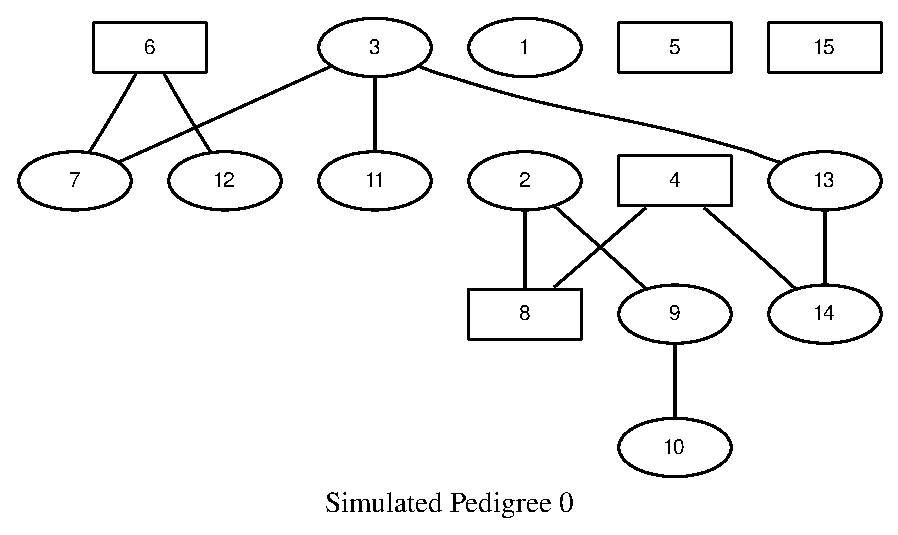
\includegraphics[width=4in]{simulatedPedigree.eps}
    \caption{Simulated pedigree using default options}
    \label{fig:example-simulated-pedigree}
  \end{center}
\end{figure}
\var{simulate\_mp} is a flag indicating whether or not simulated animals may have missing parents. When missing parents are allowed, animals may have no, one, or both parents unknown. The related parameter, \var{simulate\_pmd}, specifies the number of times parents should be sampled at random when trying to satisfy all of the simulation constraints. If parents are sampled \var{simulate\_pmd} times without satisfying the rules in place, both parents are set to missing, even if missing parents are not permitted. Other constraints include allowing/forbidding parent-offspring (\var{simulate\_po}) and/or full sib (\var{simulate\_fs}) matings.

\chapter{Input and Output}
\label{cha:inputoutput}
\begin{quote}
The only legitimate use of a computer is to play games. --- Eugene Jarvis
\end{quote}
\section{Overview}\label{sec:io-overview}
Getting data into and out of programs, while extremely important to end-users, is often challenging. \PyPedal{} is able to load pedigrees from, and save them to, from a number of different sources. A list of supported input and output methods may be found in Table \ref{tbl:io-methods}.
\begin{center}
    \tablecaption{\PyPedal{} input and output methods.}
    \tablefirsthead{\hline Direction & Source & Description \\ \hline}
    \tablehead{\hline Direction & Source & Description \\ \hline}
    \tabletail{\hline \multicolumn{3}{l}{\small\sl continued on next page} \\ \hline}
    \tablelasttail{\hline}
    \label{tbl:io-methods}
    \begin{xtabular}{l|p{1in}|p{3in}}
    Input & db & Load an ASDx-formatted data from an SQLite database \\
     & fromgraph & Load a pedigree from an instance of an XDiGraph object (not a file) \\
     & gedcomfile & Load a pedigree from a GEDCOM 5.5 file \\
     & graphfile & Load a pedigree from an adjacency list using the read_adjlist() function from the NetworkX module \\
     & simulate & Simulate a pedigree rathen that loading it from a file \\
     & textstream & Load a pedigree from a string contaiing animal records \\
    Output & save & Save a pedigree with user-specified filenames, pedigree format codes, and separators \\
     & savedb & Save a pedigree to a database table \\
     & savegedcom & Save a pedigree to a GEDCOM 5.5 file \\
     & savegedcom & Save a pedigree to a GENES 1.20 file (DBASE III format) \\
     & savegraph & Save a pedigree to a file as an adjacency list \\
    \end{xtabular}
\end{center}
It has evolved over time that the input methods are implemented as cases of \samp{pedsource} in the \method{NewPedigree::load()} method, while output methods are implemented as individual methods of \method{NewPedigree}. While it is quite straightforward to add new methods for pedigree output, it is trickier to add new input sources. The greater difficulty in adding new input sources is largely attributable to the mysterious workings of the \method{NewPedigree::preprocess()} method, which walks through input line-by-line to load the pedigree and perform a number of integrity checks. Once the data are loaded into a \method{NewPedigree} object it is easy to output them because there is no need to check the integrity of the pedigree and relationships among the records in the pedigree. If you want to implement a new input source the sanity-saving way to go is to get the data into a list that you can pass to \method{preprocess()}; \method{preprocess()} can then walk the list as it would walk through the lines of an input file.

Database operations are discussed in their own section at the end of this chapter.

\section{Input}\label{sec:io-input}\index{input}
The process of data input hsa been made as simple as is reasonably possible, but it is ultimately the responsibility of the user to prepare their data. Most people will load their data from a simple text file, with one pedigree entry per line. \index{input!integrity checks}A number of pedigree integrity checks are performed when the data are loaded. First, the pedigree format string (Section \ref{sec:pedigree-format-codes}) is checked for validity and compared to a line of data to make sure that the specfied number of colums of data exist. Once that check is passed individual records are loaded and checked one at a time. As individual records are vvalidated they are added to the pedigree. Duplicate records are eliminated, parents that appear in the pedigree but do not have their own record in the inpur data are added to the pedigree, and sexes are checked (animals cannot appear as both sires and dams). If animal IDs are strings they are hashed to get numeric IDs for use in pedigree reordering and renumbering.

If you used an earlier version of \PyPedal{} you may have added a pedigree format string to your pedigree file. You do not need to include that string in the current version of \PyPedal{}, and if \method{preprocess()} sees one while reading a pedigree file it will ignore it. You may include comment lines in your file as well; they will also be ignored.

\subsection{Graph Objects}\label{sec:io-input-xdigraph}\index{input!graph objects}
Pedigrees can be represented as a type of mathematical object called a directed graph (digraph; not to be confused with visualizations of data). The \class{NetworkX} module provides Python tools for working with digraphs, and \PyPedal{} provides a convenient way for loading a pedigree from an instance of an \class{{XD}i{G}raph} object.
\begin{verbatim}
example = pyp_newclasses.loadPedigree(optionsfile='new_networkx.ini')
ng = pyp_network.ped_to_graph(example)
options = {}
options['pedfile'] = 'dummy'
options['pedformat'] = 'asd'
example2 = pyp_newclasses.loadPedigree(options,pedsource='graph',pedgraph=ng)
example2.metadata.printme()
\end{verbatim}
You can see from the printout of the metadata from the new pedigree, \samp{example2}, that the graph \samp{ng} was successfully converted to a \class{NewPedigree} object.
\begin{verbatim}
Metadata for  Testing fromgraph() (dummy)
Records:                13
Unique Sires:           3
Unique Dams:            4
Unique Gens:            1
Unique Years:           1
Unique Founders:        5
Unique Herds:           1
Pedigree Code:          asd
\end{verbatim}
When considering the utility of such tools it might be helpful to recall that \PyPedal{} was written by and for use in scientific research. Perhaps that will allow the author to be forgiven a multitude of sins.

\subsection{{GEDCOM} Files}\label{sec:io-input-gedcom}\index{input!GEDCOM files}
A thorough description of support for {GEDCOM} files may be found in Appendix \ref{GEDCOM}.

\subsection{{GENES} Files}\label{sec:io-input-genes}\index{input!GENES files}
A thorough description of support for {GENES} files may be found in Appendix \ref{GENES}.

\subsection{Text Files}\label{sec:io-input-text-files}\index{input!text files}
Most users will load their pedigrees from simple text files. As an example, consider a large dog pedigree, an excerpt of which is presented below.
\begin{verbatim}
# dogID,fatherID,motherID,gender,born
64 66 67 2 1979
63 64 65 1 1982
62 191 195 2 1982
61 64 65 2 1982
...
\end{verbatim}
This pedigree can be loaded using this short program:
\begin{verbatim}
options = {}
options['pedfile'] = 'dog.ped'
options['pedname'] = 'A Large Dog Pedigree'
options['pedformat'] = 'asdgb'
if __name__ == '__main__':
    test = pyp_newclasses.loadPedigree(options)
\end{verbatim}
There are numerous examples of loading pedigrees from text files throughout this manual.

\subsection{Text Streams}\label{sec:io-input-text-streams}\index{input!text streams}
There are some use cases, such as web services, for which it may be desirable to load pedigrees from strings rather than from files. This is done by passing the \function{pedsource}\index{pedsource} keyword to \function{pyp_newclasses.loadPedigree} with a value of \samp{textstream}, along with a string named \samp{pedstream}:
\begin{verbatim}
options = {}
options['pedfile'] = ''
options['messages'] = 'verbose'
options['pedformat'] = 'ASD'

if __name__ == "__main__":
    pedstream = 'a1,s1,d1\na2,s2,d2\na3,a1,a2\n'
    test = pyp_newclasses.loadPedigree(options,pedsource='textstream',pedstream=pedstream)
\end{verbatim}
Only ASD-formatted pedigrees can be loaded this way, individual IDs are separated with commas, and successive records are separated by newlines. These restrictions are hard-coded into the \method{NewPedigree::load()} method. All records must contain a newline, including the last record in the string! You must also set the \samp{pedfile} option to some value, even if that value is just an empty string as in the example.

The expected use case is that the pedigree would be retrieved from a database, and the result set from the SQL query converted into a string. There is an upper bound on the size of pedigree that can be loaded from a stream based on the physical memory available on your platform, and extremely large pedigrees should be loaded from a text file. 

\section{Output}\label{sec:io-output}\index{output}
\subsection{{GEDCOM} Files}\label{sec:io-output-gedcom}\index{output!GEDCOM files}
A thorough description of {GEDCOM} file exportation may be found in Appendix \ref{GEDCOM}.

\subsection{{GENES} Files}\label{sec:io-output-genes}\index{output!GENES files}
A thorough description of {GENES} file exportation may be found in Appendix \ref{GENES}.

\subsection{Graph Objects}\label{sec:io-output-xdigraph}\index{output!graph objects}
The \method{NewPedigree::savegraph()} save a pedigree to a file as an adjacency list, which is a commonly-used format for describing digraphs. If the pedigree has already been converted to a digraph pass it using the \var{pedgraph} argument; otherwise, the method will call the appropriate converter:
\begin{verbatim}
test.savegraph(pedoutfile='test.adj')
\end{verbatim}
The file \samp{test.adj} has the following comments:
\begin{verbatim}
# sqlite.py
# GMT Tue Mar  4 20:38:52 2008
# Text Stream
1 5
2 6
3 5
4 6
5 7
6 7
7
\end{verbatim}
This example demonstrates that there can be a considerable loss of information when going from a \PyPedal{} pedigree to some other way of representing the pedigree, such as a graph.

\subsection{Text Files}\label{sec:io-output-text-files}\index{output!text files}
The \method{NewPedigree::save()} method writes a \PyPedal{} pedigree to a user-specified file based on a pedigree format string and optional column separator provided by the user. By default, the pedformat is \samp{asd} and the sepchar is \samp{ }. Any attribute of a \method{NewAnimal} object can be written to an output file.

\method{NewPedigree::save()} tries never to overwrite your data. If you do not pass a filename argument a file whose name is derived from, but not the same as, the original pedigree filename will be used. The string \samp{\_saved} will be appended to the filename in order to distinguish it from the original pedigree file.

There are a few points that you need to be aware of when using \method{NewPedigree::save()}. First, you may use any column separator you choose but the empty string
(\texttt{sepchar=''}); if you try and do this the sepchar will be changed to the global default (currently \samp{ }), and a message written to the log. That means
that there is no way for you to run all of the columns in your pedigree file together such that they cannot easily be separated. Sorry.  You can use anoy other string
you like to separate your columns (spaces, columns, and tabs have been tested).It IS possible to write an
incomplete pedigree file, that is, a file which does not include animal, sire, and dam information. \PyPedal{} checks the pedformat to see if it contains either
\texttt{'asd'} or \texttt{'ASD'} and warns you if it does not, but it will happily write the file you tell it to. The burden is on you, the user, to make sure that
your output file contains all of the information you want. Finally, you can write whatever attribute you like to whichever column you like in the output file. For the
sake of your sanity I strongly recommend that you always place the animal, sire, and dam IDs in the first three columns, but you're an adult and may do what you like.

Maybe a couple of examples will help clear that up. Here's the simplest case, taking defaults:
\begin{verbatim}
test.save('test_save_asd.ped')
\end{verbatim}
gets you the result:
\begin{verbatim}
# test_save_asd.ped created by PyPedal at Tue Sep 28 16:39:36 2010
# Current pedigree metadata:
#       pedigree file: test_save_asd.ped
#       pedigree name: Untitled
#       pedigree format: asd
#       NOTE: Animal, sire, and dam IDs are RENUMBERED IDs, not original IDs!
# Original pedigree metadata:
#       pedigree file: ../simulated_pedigree.ped
#       pedigree name: Untitled
#       pedigree format: asdxg
1 0 0
2 0 0
3 0 0
4 0 0
5 0 0
...
21 19 10
22 9 12
23 1 10
24 1 21
25 13 8
\end{verbatim}
Note the friendly header to tell you what you've got and from where it came. The note about renumbere IDs is particularly important -- if
the \texttt{pedigree\_is\_renumbered} flag is set then you will get this message to alert you that comparing this file against your original
source file may give conflicting results. Well, they're not really conflicting, but if you compare renumbered with not-renumbered IDs the
you may assume there's some kind of problem when really there is not. Original and renumbered pedigrees are mathematically equivalent assuming
that there were no errors in the original file that were corrected by \PyPedal{}. Isn't that reassuring? From here on out I will not show the
header, and will include only the first five data rows in the file for the sake of brevity (like I've ever let that stop me before). You can get
the same thing as a CSV using the sepchar argument:
\begin{verbatim}
test.save('test_save_asd_csv.ped', sepchar=',')
\end{verbatim}
which produces:
\begin{verbatim}
1,0,0
2,0,0
3,0,0
4,0,0
5,0,0
...
\end{verbatim}
Sometimes you want to go all the way and dump everything into a file. This is like one of those pizzas with every variety of cured meat known to
food science piled up on top. Here you go:
\begin{verbatim}
test.save('test_save_combo_all.ped', pedformat = 'asdgxbfrnylepASDLhHu')
\end{verbatim}
which gives you what you asked for, even if many of the values are not particularly interesting:
\begin{verbatim}
1 0 0 0 m 01011900 0.0 Unknown_Breed 7 1900 0 -999 -999.0 7 Unknown_Name Unknown_Name ['1900000000000000071__1', '1900000000000000071__2'] 57361b5fd9993f00437fbe4c4675feca Unknown_Herd
2 0 0 0 m 01011900 0.0 Unknown_Breed 6 1900 0 -999 -999.0 6 Unknown_Name Unknown_Name ['1900000000000000061__1', '1900000000000000061__2'] 57361b5fd9993f00437fbe4c4675feca Unknown_Herd
3 0 0 0 m 01011900 0.0 Unknown_Breed 5 1900 0 -999 -999.0 5 Unknown_Name Unknown_Name ['1900000000000000051__1', '1900000000000000051__2'] 57361b5fd9993f00437fbe4c4675feca Unknown_Herd
4 0 0 0 f 01011900 0.0 Unknown_Breed 3 1900 0 -999 -999.0 3 Unknown_Name Unknown_Name ['1900000000000000031__1', '1900000000000000031__2'] 57361b5fd9993f00437fbe4c4675feca Unknown_Herd
5 0 0 0 f 01011900 0.0 Unknown_Breed 2 1900 0 -999 -999.0 2 Unknown_Name Unknown_Name ['1900000000000000021__1', '1900000000000000021__2'] 57361b5fd9993f00437fbe4c4675feca Unknown_Herd
...
\end{verbatim}
Okay, I get it. You're like the Nigel Tufnel of Missouri -- you want to see something that goes to 11. I pondered this for a while. You've read this far
and deserve to be rewarded. So I tried to think of the most awesomest thing that I could think of. So here you go, LSU fans, straight from Death Valley
by way of Beltsville, MD:
\begin{verbatim}
test.save('test_save_peterson.ped', pedformat = 'asd', sepchar = '...Kneel before Zod!...'
\end{verbatim}
Maybe Patrick Peterson is really into genealogy -- you never know -- stop looking at me like that! This is a perfectly cromulent example of the extremes to
which the sepchar argument can be pushed:
\begin{verbatim}
1...Kneel before Zod!...0...Kneel before Zod!...0
2...Kneel before Zod!...0...Kneel before Zod!...0
3...Kneel before Zod!...0...Kneel before Zod!...0
4...Kneel before Zod!...0...Kneel before Zod!...0
5...Kneel before Zod!...0...Kneel before Zod!...0
...
\end{verbatim}
You're thinking, "My eyes! Why would he do that?!" The same reason Zod gave us a little Heisman pose in the end zone after returning a West Virginia kickoff for 6 --
because I can. (This kind of writing is probably going to get me in trouble one day, but the boss is out of town and there's no one here to rein-in my behavior!) Wait,
though. It gets better. \PyPedal{} can get all Ourboros on this unholy creation:
\begin{verbatim}
# But, wait, can this actually work?
options2 = options
options2['pedfile'] = 'test_save_peterson.ped'
options2['sepchar'] = '...Kneel before Zod!...'
options2['pedformat'] = 'asd'
test2 = pyp_newclasses.loadPedigree(options2)
\end{verbatim}
When you run this bit of code you see that it poses no problem at all for \PyPedal{}. Perhaps political dissidents can communicate secretly by doing strange things
with \var{sepchar}, although it's more likely that PhD students will find a clever way to abuse MS students with it, instead.
\begin{verbatim}
[INFO]: Logfile untitled_pedigree.log instantiated.
[INFO]: Preprocessing test_save_peterson.ped
[INFO]: Opening pedigree file test_save_peterson.ped
        [INFO]: Renumbering pedigree at Wed Sep 29 13:42:05 2010
                [INFO]: Reordering pedigree at Wed Sep 29 13:42:05 2010
                [INFO]: Renumbering at Wed Sep 29 13:42:05 2010
                [INFO]: Updating ID map at Wed Sep 29 13:42:05 2010
        [INFO]: Assigning offspring at Wed Sep 29 13:42:05 2010
[INFO]: Creating pedigree metadata object
        [INFO]:  Instantiating a new PedigreeMetadata() object...
        [INFO]:  Naming the Pedigree()...
        [INFO]:  Assigning a filename...
        [INFO]:  Attaching a pedigree...
        [INFO]:  Setting the pedcode...
        [INFO]:  Counting the number of animals in the pedigree...
        [INFO]:  Counting and finding unique sires...
        [INFO]:  Counting and finding unique dams...
        [INFO]:  Setting renumbered flag...
        [INFO]:  Counting and finding unique generations...
        [INFO]:  Counting and finding unique birthyears...
        [INFO]:  Counting and finding unique founders...
        [INFO]:  Counting and finding unique herds...
        [INFO]:  Detaching pedigree...
Metadata for Untitled (test_save_peterson.ped)
        Records:                25
        Unique Sires:           7
        Unique Dams:            7
        Unique Gens:            1
        Unique Years:           1
        Unique Founders:        6
        Unique Herds:           1
        Pedigree Code:          asd
\end{verbatim}
How's that for the strangest thing you're likely to see all day? I'm not suggesting that you seriously use column separators the way I just did, but this
example does show that you can do some unusual things with \PyPedal{}, and perhaps you will come up with something very useful because of that flexibility.
If nothing else, you now have a greater appreciation of what you can do with a dynamic language and questionable processing of user inputs. Remember, never
trust any data a user gives you. They're a shifty lot, users.

\subsection{Text Streams}\label{sec:io-output-text-streams}\index{output!text streams}
\method{NewPedigree::tostream()} returns a text stream from an instance of a \class{NewPedigree} object. The text stream contains an ASD-formatted pedigree as a string in which individual IDs are separated by commas and successive records are separated by newlines.
\begin{verbatim}
>>> pedstream = 'a1,s1,d1\na2,s2,d2\na3,a1,a2\n'
>>> test = pyp_newclasses.loadPedigree(options,pedsource='textstream',pedstream=pedstream)
>>> pedstream2 = test.tostream()
>>> print pedstream2
'd1,0,0\nd2,0,0\ns1,0,0\ns2,0,0\na2,s2,d2\na1,s1,d1\na3,a1,a2\n'
\end{verbatim}
Note that in this example the input and output text streams differ because the input stream did not include pedigree entries for all animals in the pedigree (for example, sire \samp{s1}). Recall that \PyPedal{} adds missing entries for parents when the pedigree is loaded.

\section{Databases}\label{sec:io-databases}\index{databases}
\PyPedal{} is able to load pedigrees from, and save them to, three databases:
\href{http://www.mysql.com/}{MySQL}, \href{http://www.postgresql.org/}{Postgres},
and \href{http://sqlite.org/}{SQLite}. \PyPedal{} uses the 
\href{http://phplens.com/lens/adodb/adodb-py-docs.htm}{ADOdb for Python} database
abstraction tool, which is distributed with \PyPedal{} to talk to these databases.
Additional databases are supported by ADOdb and require only minor changes to the
connection strings in the \function{connectToDatabase} function in the \module{pyp_db}
module in order to work with \PyPedal{} as well.

A list of the database-related keywords may be found in Table \ref{tbl:db-parms}.
\begin{center}
    \tablecaption{Database parameters.}
    \tablefirsthead{\hline Parameter & Default & Description \\ \hline}
    \tablehead{\hline Parameter & Default & Description \\ \hline}
    \tabletail{\hline \multicolumn{3}{l}{\small\sl continued on next page} \\ \hline}
    \tablelasttail{\hline}
    \label{tbl:db-parms}
    \begin{xtabular}{l|p{1in}|p{3in}}
    database\_debug & False & Toggle debugging messages in the database module on and off. \\
    database\_host & 'localhost' & The server on which the database is running. \\
    database\_name & 'pypedal' & The name of the database to be used. \\
    database\_passwd & 'anonymous' & The password needed to connect to your database. \\
    database\_port & '' & The port on which your databse is listening for connections (needed only for Postgres). \\
    database\_table & 'filetag' (See: Table \ref{tbl:options}) & The name of the database table to which the current pedigree will be written. \\
    database\_type & 'sqlite' & The type of database you are using ('mysql'|'postgres'|'sqlite'). \\
    database\_user & 'anonymous' & The name of a user with access rights to your database.  \\
    \end{xtabular}
\end{center}

\subsection{Input from Databases}\label{sec:io-input-database}\index{input!databases}
\PyPedal{} can load ASDx-formatted pedigrees from an SQLite database using \samp{pedsource='db'}. The pedigree will be loaded from the database and table specified in the \var{database\_name} and \var{dbtable\_name} variables. Consider the following example:
\begin{verbatim}
test = pyp_newclasses.loadPedigree(options,pedsource='db')
test.metadata.printme()
\end{verbatim}
This produces the output:
\begin{verbatim}
Metadata for  DB Stream ()
    Records:                7
    Unique Sires:           3
    Unique Dams:            3
    Unique Gens:            1
    Unique Years:           1
    Unique Founders:        4
    Unique Herds:           1
    Pedigree Code:          ASDx
\end{verbatim}
Note that user-supplied values of the pedigree format string will be over-written by the \method{load()} method and do not affect database processing. Database importation is hard-coded to accept only pedigrees in that format.

\index{databases!new input sources}It is possible to load pedigrees from a databse with a format different than that exected by \PyPedal{}, but it requires that you make changes to the \class{NewPedigree} class's \method{load} method. Consider the database-loading code that is located at about line 250 of \texttt{pyp_newclasses.py}:
\begin{verbatim}
251  elif pedsource == 'db':
252      self.kw['pedformat'] = 'ASDx'
253      self.kw['sepchar'] = ','
...
259      try:
260          # Connect to the database
261          if pyp_db.doesTableExist(self):
262            conn = pyp_db.connectToDatabase(self)
263              if conn:
264                  sql = 'SELECT * FROM %s' % ( self.kw['database_table'] )
265                  dbstream = conn.GetAll(sql)
\end{verbatim}
In order to load data from your own database you must change the pedigree format string
on line 252 to match the pedigree you want to load (see Table
\ref{tbl:pedigree-format-codes} for a list of pedigree format codes). You then need to
change the SQL statement on line 264 to match the column names in your database and the
order of fields in your pedigree format string. The animal, sire, and dam IDs,
respectively, should always  be the first three columns in your records. The query
results are stored as a list of tuples in \var{dbstream} and will be unpacked in the
\method{preprocess} method (\textit{cf.} line 864).

Please note that while I will try and answer questions about the way in which \PyPedal{}
handles loading pedigrees from databases, I cannot answer detailed questions about 
databases to which I do not ave access. You should carefully test your custom queries in
SQL to ensure that they are working correctly before adding them to \PyPedal{}. Also,
please check your pedigree format string to make sure that it matches your query.

\subsection{Output to Databases}\label{sec:io-output-database}\index{output!databases}
\PyPedal{} can write \class{NewPedigree} pedigrees to ASDx-formatted SQLite tables using the \method{NewPedigree::savedb()} method. The following program will result in the creation of a table named \samp{test\_save} in the database \samp{test\_pypedal\_save}.
\begin{verbatim}
test.kw['database_name'] = 'test_pypedal_save'
test.kw['dbtable_name'] = 'test_save'
test.savedb()
\end{verbatim}
The pedigree is saved to the database and table specified in the \var{database\_name} and \var{dbtable\_name} variables. If the specified table already exists then the records from the current pedigree will be added to the table. If you want to overwrite the existing database then you need to pass \samp{drop=True} in the call to method{savedb}:
\begin{verbatim}
test.savedb(drop=True)
\end{verbatim}
While this may strike some users as unexpected behavior it is based on the idea that you should never lose data unexpectedly. If you use only the defaults you will never lose data. However, if you try and save a renumbered pedigree on top of another renumbered pedigree you will run into problems because animal IDs are used as primary keys, and you will have constraint violations.

\index{databases!new output destinations}It is possible to save pedigrees to a databse
with a format different than that exected by \PyPedal{}, but it is a little harder than
changeing pedigree input. Changing the output table requires that you change the
\class{NewPedigree} class's \method{savesb} method. Consider the code that begins on or
about line 590 of \texttt{pyp_newclasses.py} in \method{savesb}:
\begin{verbatim}
591  sql = 'create table %s ( \
592      animalName   varchar(128) primary key, \
593      sireName     varchar(128), \
594      damName      varchar(128), \
595      sex          char(1) \
596      );' % ( self.kw['database_table'] )
\end{verbatim}
You need to rewrite this statement to add or remove columns; the SQL for a tavble that 
includes all fields in a \class{NewAnimal} object may be found in the 
\function{createPedigreeTable} function of the \module{pyp\_db module}. Note that not 
every field in a \class{NewAnimal} object has a corresponding pedigree format code. 
Consult Table \ref{sec:pedigree-format-codes} for appropriate codes.

Once you've updated the SQL used to create your custom pedigree table you will also need to change the code which prepares the input for writing to the database. This code is found on or about about line 617 in \method{savesb}:
\begin{verbatim}
617  sql = "INSERT INTO %s ( animalName, sireName, damName, sex ) VALUES ('%s', '%s', '%s', '%s')" % ( self.kw['database_table'], an, si, da, p.sex )
\end{verbatim}
Note that you will need to make appropriate casts yourself. For example, you will want 
to cast things that are stored as integers or reals to make sure that you don't violate 
a column constraint. You must enclose strings in single-quotation marks ('') yourself. 

By default \PyPedal{} saves pedigrees in \samp{ASD} format. If you want to save your pedigree in \samp{asd} format then you will need to change the code on or about line 610 from:
\begin{verbatim}
610  an = p.name
611  si = p.sireName
612  da = p.damName
\end{verbatim}
to:
\begin{verbatim}
610  an = p.animalID
611  si = p.sireID
612  da = p.damID
\end{verbatim}
It is better to add a new method supporting your output format to \class{NewAnimal}   rather than changing the \method{savedb} method.

\chapter{Working with Pedigrees}
\label{cha:computing}
\begin{quote}
 Are you quite sure that all those bells and whistles, all those wonderful facilities of your so called powerful programming languages, belong to the solution set rather than the problem set? --- Edsger Dijkstra
\end{quote}
\section{Overview}\label{sec:computing-overview}\index{working with pedigrees}
In Chapter \ref{cha:inputoutput} you learned how to get your pedigree data loaded into \PyPedal{}. This chapter will show you what you can do with the pedigree once it is loaded. The examples in this chapter assumes that you are working with a reordered and renumbered pedigree (see Section \ref{sec:methodology-reordering-and-renumbering} for additional details).

In order to get the most out of your pedigrees you need to understand the basic structure of a \PyPedal{} pedigree, which consists of two components: the pedigree itself, which is composed of a list of \class{NewAnimal} objects, and metadata, which is data about the animals contained in the pedigree. Some calculations are performed on the animal records directly, while others use the metadata, or some combination of the two. The fundamental goal of \PyPedal{} is to provide the user with tools for asking questions about their pedigrees.

The following discussion will use the following pedigree taken from Boichard et al. \citeyear{ref352}:
\begin{verbatim}
# pedformat: asdg
1 0 0 1
2 0 0 1
3 0 0 1
4 0 0 1
5 1 2 2
6 3 4 2
7 5 6 3
8 5 6 3
9 5 6 3
10 5 6 3
11 5 6 3
12 5 6 3
13 5 6 3
14 5 6 3
\end{verbatim}
Many of the subsequent code snippets are taken from the \samp{new\_methods.py} example program (see: Appendix \ref{cha:example-programs}). 

\section{Inbreeding and Relationships}\label{sec:computing-inbreeding}\index{working with pedigrees!inbreeding and relationships}

\begin{verbatim}
inbr = pyp_nrm.inbreeding(example)
print 'inbr: ', 
>>> inbr:  {
    'fx': {1: 0.0, 2: 0.0, 3: 0.0, 4: 0.0, 5: 0.0, 6: 0.0, 7: 0.0,
        8: 0.0, 9: 0.0, 10: 0.0, 11: 0.0, 12: 0.0, 13: 0.0, 14: 0.0},
    'metadata': {
        'nonzero': {'f_max': 0.0, 'f_avg': 0.0, 'f_rng': 0.0,
            'f_sum': 0.0, 'f_min': 0.0, 'f_count': 0},
        'all': {'f_max': 0.0, 'f_avg': 0.0, 'f_rng': 0.0, 'f_sum': 0.0,
            'f_min': 0.0, 'f_count': 14}
        }
    }
\end{verbatim}
The dictionary returned by \function{inbreeding()} contains two dictionaries: \samp{fx} contains coefficients of inbreeding keyes to animal IDs, and \samp{metadata} contains summary information about the coefficients of inbreeding in the pedigree. \samp{metadata} also contains two dictionaries: \samp{nonzero} contains summary statostics only for animals with non-zero coefficients of inbreeding, and \samp{all} contains statistics for all animals.

Relationship metadata, similar to the inbreeding metadata described above but for coefficients of relationship, are available but not calculated by default. 
\begin{verbatim}
inbr,reln = pyp_nrm.inbreeding(example,rels=1)
print 'reln: ', reln
>>> reln:  {'r_nonzero_count': 10, 'r_nonzero_avg': 0.40000000000000002,
    'r_min': 0.25, 'r_sum': 4.0, 'r_avg': 0.19047619047619047, 'r_max': 0.5,
    'r_count': 21, 'r_rng': 0.25}
\end{verbatim}
The dictionary of relationship metadata returned by \function{inbreeding()} also contains statistics for zero and non-zero coefficients of relationship. On the example presented above the pedigree contains 

Relationship metadata are not guaranteed to be correct when \samp{method = 'vanraden'} is used. This is because \function{inbreeding_vanraden()} uses a speed-up when there are full-sibs in the pedigree to avoid repeating calculations. The metadata should be reasonably accurate for pedigrees with few or no full-sibs. The summary statistics will not be very accurate in the case of pedigrees that contain lots of full-sibs.

The relationship metadata do not include individual pairwise relationships. In order to associate those with your pedigree you must create a \class{NewAMatrix} object, form the numerator relationship matrix (NRM), and attach it to the pedigree:
\begin{verbatim}
options = {}
...
example = pyp_newclasses.loadPedigree(options)
example.nrm = pyp_newclasses.NewAMatrix(example.kw)
example.nrm.form_a_matrix(example.pedigree)
\end{verbatim}
If you know when you load the pedigree file  that you want to calculate and store the NRM you can save a little typing by setting the \samp{form\_nrm} option:
\begin{verbatim}
options = {}
options['form_nrm'] = 1
...
example = pyp_newclasses.loadPedigree(options)
\end{verbatim}
If you want to inspect the NRM you can use \samp{example.nrm.printme()} to print the matrix to the screen, which is probably not a particularly good idea for large matrices.
\begin{verbatim}
[[ 1.   0.   0.   0.   0.5  0.   0.25 0.25 0.25 0.25 0.25 0.25 0.25 0.25]
 [ 0.   1.   0.   0.   0.5  0.   0.25 0.25 0.25 0.25 0.25 0.25 0.25 0.25]
 [ 0.   0.   1.   0.   0.   0.5  0.25 0.25 0.25 0.25 0.25 0.25 0.25 0.25]
 [ 0.   0.   0.   1.   0.   0.5  0.25 0.25 0.25 0.25 0.25 0.25 0.25 0.25]
 [ 0.5  0.5  0.   0.   1.   0.   0.5  0.5  0.5  0.5  0.5  0.5  0.5  0.5 ]
 [ 0.   0.   0.5  0.5  0.   1.   0.5  0.5  0.5  0.5  0.5  0.5  0.5  0.5 ]
 [ 0.25 0.25 0.25 0.25 0.5  0.5  1.   0.5  0.5  0.5  0.5  0.5  0.5  0.5 ]
 [ 0.25 0.25 0.25 0.25 0.5  0.5  0.5  1.   0.5  0.5  0.5  0.5  0.5  0.5 ]
 [ 0.25 0.25 0.25 0.25 0.5  0.5  0.5  0.5  1.   0.5  0.5  0.5  0.5  0.5 ]
 [ 0.25 0.25 0.25 0.25 0.5  0.5  0.5  0.5  0.5  1.   0.5  0.5  0.5  0.5 ]
 [ 0.25 0.25 0.25 0.25 0.5  0.5  0.5  0.5  0.5  0.5  1.   0.5  0.5  0.5 ]
 [ 0.25 0.25 0.25 0.25 0.5  0.5  0.5  0.5  0.5  0.5  0.5  1.   0.5  0.5 ]
 [ 0.25 0.25 0.25 0.25 0.5  0.5  0.5  0.5  0.5  0.5  0.5  0.5  1.   0.5 ]
 [ 0.25 0.25 0.25 0.25 0.5  0.5  0.5  0.5  0.5  0.5  0.5  0.5  0.5  1.  ]]
\end{verbatim}
If you want to get the pairwise relationship between two animals you need to use their renumbered IDs and subtract 1 (because the array is zero-indexed). For example, if you wanted the coefficient of relationship between animals 2 and 5 (an individual and its sire) you would use the indices \samp{1} and \samp{4}:
\begin{verbatim}
print example.nrm.nrm[1][4]
>>> 0.5
\end{verbatim}
The NRM is symmetric, which means that \samp{nrm{[1]}{[4]}} and \samp{nrm{[4]}{[1]}} are identical.
\begin{verbatim}
print example.nrm.nrm[1][4]
>>> 0.5
print example.nrm.nrm[5][1]
>>> 0.5
\end{verbatim}
You can also easily save the NRM to a file for future reference:
\begin{verbatim}
example.nrm.save('Amatrix.txt')
\end{verbatim}
If you're from Missouri you can verify that the contents of \samp{Amatrix.txt} are:
\begin{verbatim}
1.0  0.0  0.0  0.0  0.5 0.0 0.25 0.25 0.25 0.25 0.25 0.25 0.25 0.25
0.0  1.0  0.0  0.0  0.5 0.0 0.25 0.25 0.25 0.25 0.25 0.25 0.25 0.25
0.0  0.0  1.0  0.0  0.0 0.5 0.25 0.25 0.25 0.25 0.25 0.25 0.25 0.25
0.0  0.0  0.0  1.0  0.0 0.5 0.25 0.25 0.25 0.25 0.25 0.25 0.25 0.25
0.5  0.5  0.0  0.0  1.0 0.0 0.5  0.5  0.5  0.5  0.5  0.5  0.5  0.5
0.0  0.0  0.5  0.5  0.0 1.0 0.5  0.5  0.5  0.5  0.5  0.5  0.5  0.5
0.25 0.25 0.25 0.25 0.5 0.5 1.0  0.5  0.5  0.5  0.5  0.5  0.5  0.5
0.25 0.25 0.25 0.25 0.5 0.5 0.5  1.0  0.5  0.5  0.5  0.5  0.5  0.5
0.25 0.25 0.25 0.25 0.5 0.5 0.5  0.5  1.0  0.5  0.5  0.5  0.5  0.5
0.25 0.25 0.25 0.25 0.5 0.5 0.5  0.5  0.5  1.0  0.5  0.5  0.5  0.5
0.25 0.25 0.25 0.25 0.5 0.5 0.5  0.5  0.5  0.5  1.0  0.5  0.5  0.5
0.25 0.25 0.25 0.25 0.5 0.5 0.5  0.5  0.5  0.5  0.5  1.0  0.5  0.5
0.25 0.25 0.25 0.25 0.5 0.5 0.5  0.5  0.5  0.5  0.5  0.5  1.0  0.5
0.25 0.25 0.25 0.25 0.5 0.5 0.5  0.5  0.5  0.5  0.5  0.5  0.5  1.0
\end{verbatim}
Information on the endianness and precision of the data in the array are lost, so this is not a good way to archive data or move data between machines with different endianness. The data are always written in C (row major) order. For better performance you can set the \samp{nrm\_format} option to \samp{binary}, which will use a binary file form.

Finally, if you're going to work on the exact same pedigree later you can load \samp{Amatrix.txt} and avoid having to recalculate the NRM entirely:
\begin{verbatim}
example.nrm2 = pyp_newclasses.NewAMatrix(example.kw)
example.nrm2.load('Amatrix.txt')
example.nrm2.printme()
\end{verbatim}
Since we've loaded \samp{Amatrix.txt} into a second NRM (\samp{nrm2}) attached to our pedigree it's straightforward, if tedious, to verify that the two NRM contain the same values.

\section{Matings}\label{sec:computing-matings}\index{working with pedigrees!matings}
There are a number of questions you might wish to ask that involve matings, such as, ``What is the minimum-inbreeding mating among this set of individuals?''. Several routines in \module{pyp\_metrics}.

Suppose you were considering a mating between animals 5 (index 4) and 14 (index 13), which is a sire-daughter mating. How would you go about this? You simply call \method{pyp\_metrics.mating\_coi()}:
\begin{verbatim}
print '\tCalling mating_coi() at %s' % ( pyp_nice_time() )
f = pyp_metrics.mating_coi(example.pedigree[4].animalID,
    example.pedigree[13].animalID,example,1)
print f
\end{verbatim}
which produces the output:
\begin{verbatim}
Calling mating_coi() at Wed Mar  5 11:31:30 2008
0.25
\end{verbatim}
We don't need \PyPedal{} to tell us the coefficient of inbreeding of such a simple mating, but the calculations can be complex for more complicated cases. While you can do all of the necessary computations ``by hand'', \method{pyp\_metrics.mating\_coi()} takes care of that for you by adding a new dummy animal to the pedigree with the proposed parents, calculating the coefficient of inbreeding of that mating, deleting the dummy animal from the pedigree, and returning the coefficient of inbreeding.

\PyPedal{} takes things one step further, allowing you to work with groups of proposed matings at one time using \method{pyp\_metrics.mating\_coi\_group()}. Internally it works similarly to \method{pyp\_metrics.mating\_coi()}, although instead of passing a pair of parents you pass a list of proposed matings. The matings are of the form \samp{<parent1>\_<parent2>}. Here's an example in which we are going to consider the following three matings: 1 with 5, 1 with 14, and 5 with 14. Note how the matings are formed and appended to the \samp{matings} list in one step.
\begin{verbatim}
matings = []
matings.append('%s_%s'%(example.pedigree[0].animalID, example.pedigree[4].animalID))
matings.append('%s_%s'%(example.pedigree[0].animalID, example.pedigree[13].animalID))
matings.append('%s_%s'%(example.pedigree[4].animalID, example.pedigree[13].animalID))
fgrp = pyp_metrics.mating_coi_group(matings,example)
print 'fgrp: ', fgrp['matings']
\end{verbatim}
That code produces a list of the proposed matings with associated coefficients of inbreeding. In addition to the \samp{matings} dictionary, the \samp{fgrp} dictionary also contains a dictionary named \samp{metadata} which contains summary statistics about the proposed matings.
\begin{verbatim}
fgrp:  {'1_5': 0.25, '5_14': 0.25, '1_14': 0.125}
\end{verbatim}
\section{Relatives}\label{sec:computing-relatives}\index{working with pedigrees!relatives}
\PyPedal{} provides a number of tools for extracting information about relatives from a pedigree. Examples include: obtaining lists of the ancestors of an animal, getting lists of ancestors shared in common by a pair of animals, listing the descendants of an individual, the calculation of the additive genetic relationship between a given pair of animals, and the creation of ``subpedigrees'' containing only specified animals.

It is easy to obtain a list of an animal's relatives using \method{pyp\_metrics.related\_animals()}:
\begin{verbatim}
list_a = pyp_metrics.related_animals(example.pedigree[6].animalID,example)
list_b = pyp_metrics.related_animals(example.pedigree[13].animalID,example)
\end{verbatim}
produces a list of each animal's relatives:
\begin{verbatim}
[5, 1, 2]
[14, 5, 1, 2, 6, 3, 4]
\end{verbatim}
\method{pyp\_metrics.common\_ancestors()} is used to get a list of the common ancestors of two animals, say animals \samp{5} and \samp{14} (remember that this pedigree is renumbered, and that Python lists are indexed from 0, so we need to offset the animal IDs by 1 to get the correct animal IDs).
\begin{verbatim}
list_r = pyp_metrics.common_ancestors(example.pedigree[4].animalID,example.pedigree[13].ani
malID,example)
print list_r
\end{verbatim}
Results are returned as lists:
\begin{verbatim}
[1, 2, 5]
\end{verbatim}
If you've already obtained ancestor lists for a given pair of animals in which you're interested you can also obtain a list of common ancestors using Python sets, which avoids performing calculations more than needed:
\begin{verbatim}
>>> set_a = set(list_a)
>>> set_b = set(list_b)
>>> set_c = set_a.intersection(set_b)
>>> set_c
set([1, 2, 5])
>>> list_c = list(set_c)
>>> list_c
[1, 2, 5]
\end{verbatim}
A list of descendants can be obtained by calling \method{pyp\_metrics.descendants()}, which returns a dictionary:
\begin{verbatim}
>>> pyp_metrics.descendants(5,example,{})
{7: 7, 8: 8, 9: 9, 10: 10, 11: 11, 12: 12, 13: 13, 14: 14}
\end{verbatim}
However, it is improtant to note that you will not get the answer you expect unless you have either set the option \samp{set\_offspring = 1} or called \method{pyp\_utils.assign\_offspring()} after loading the pedigree. There is also a convenience function, \method{pyp\_metrics.founder\_descendants()}, for handling the special case of obtaining descendants of all of the founders in the pedigree:
\begin{verbatim}
>>> pyp_metrics.founder_descendants(example)
{1: {5: 5, 7: 7, 8: 8, 9: 9, 10: 10, 11: 11, 12: 12, 13: 13, 14: 14},
 2: {5: 5, 7: 7, 8: 8, 9: 9, 10: 10, 11: 11, 12: 12, 13: 13, 14: 14},
 3: {6: 6, 7: 7, 8: 8, 9: 9, 10: 10, 11: 11, 12: 12, 13: 13, 14: 14},
 4: {6: 6, 7: 7, 8: 8, 9: 9, 10: 10, 11: 11, 12: 12, 13: 13, 14: 14}}
\end{verbatim}
\section{Decomposition and Direct Inverses of Numerator Relationship Matrices}\label{sec:computing-decomposition}\index{numerator relationship matrix!decomposition}\index{numerator relationship matrix!direct inverses}
\PyPedal{} provides routines in the \method{pyp_nrm} module for decomposing and forming direct inverses of numerator relationship matrices (NRM). The NRM, $A$, may be written as $A=TDT'$, where $T$ is a lower triangular matrix and $D$ is a diagonal matrix \cite{ref143,ref1060}. $T$ traces the flow of genes from one generation to another, while $D$ provides variances and covariances of Mendelian sampling. Mrode \citeyear{ref224} presents a more detailed discussion of this decomposition. The examples in this section all use the pedigree presented in Table 2.1 of that work, which is contained in the file \samp{examples/new_decompose.ped}:
\begin{verbatim}
# Pedigree from Table 2.1 of
# Mrode (1996)
1 0 0
2 0 0
3 1 2
4 1 0
5 4 3
6 5 2
\end{verbatim}
The results presented below may be obtained by running the \samp{new_decompose.py} example program. The \method{pyp_nrm.a_decompose()} function takes as its argument a pedigree object and returns the matrices $T$ and $D$. The code
\begin{verbatim}
print 'Calling a_decompose()'
print '====================='
D, T  = pyp_nrm.a_decompose(example)
print 'D: ', D
print
print 'T: ', T
\end{verbatim}
produces identical answers to those presented by Mrode \citeyear{ref224} (note that outputs may have been reformatted slightly to improve readability).
\begin{verbatim}
Calling a_decompose()
=====================
D:  [[ 1.       0.       0.       0.       0.       0.     ]
 [ 0.       1.       0.       0.       0.       0.     ]
 [ 0.       0.       0.5      0.       0.       0.     ]
 [ 0.       0.       0.       0.75     0.       0.     ]
 [ 0.       0.       0.       0.       0.5      0.     ]
 [ 0.       0.       0.       0.       0.       0.46875]]

T:  [[ 1.     0.     0.     0.     0.     0.   ]
 [ 0.     1.     0.     0.     0.     0.   ]
 [ 0.5    0.5    1.     0.     0.     0.   ]
 [ 0.5    0.     0.     1.     0.     0.   ]
 [ 0.5    0.25   0.5    0.5    1.     0.   ]
 [ 0.25   0.625  0.25   0.25   0.5    1.   ]]
\end{verbatim}
It is not generally feasible to directly compute the inverse, $A^{-1}$, of large NRM. However, it is possible to formulate simple rules for computing the inverse directly from. Henderson \citeyear{ref143} presented a simple procedure for calculating $A^{-1}$ without accounting for inbreeding taking advantage of the fact that $A^{-1}=(T^{-1})'D^{-1}T^{-1}$, which is implemented as \method{pyp_nrm.form_d_nof()}:
\begin{verbatim}
print 'Calling a_inverse_dnf()'
print '======================='
Ainv = pyp_nrm.a_inverse_dnf(example)
print 'Ainv: ', Ainv
\end{verbatim}
produces $A^{-1}$ without accounting for inbreeding in the pedigree:
\begin{verbatim}
Calling a_inverse_dnf()
=======================
Ainv:  [[ 1.83333333  0.5        -1.         -0.66666667  0.          0.        ]
 [ 0.5         2.         -1.          0.          0.5        -1.        ]
 [-1.         -1.          2.5         0.5        -1.          0.        ]
 [-0.66666667  0.          0.5         1.83333333 -1.          0.        ]
 [ 0.          0.5        -1.         -1.          2.5        -1.        ]
 [ 0.         -1.          0.          0.         -1.          2.        ]]
\end{verbatim}
Quaas \citeyear{ref235} built on Henderson's earlier work by providing an algorithm for the computation of $A^{-1}$ accounting for inbreeding, which is implemented as the function  \function{pyp_nrm.a_inverse_df()}.
\begin{verbatim}
print 'Calling a_inverse_df()'
print '======================'
Ainv = pyp_nrm.a_inverse_df(example)
print 'Ainv: ', Ainv
\end{verbatim}
You will note that the numbers in this matrix are slightly different from those in the previous example. Those differences are due to the inbreeding in the pedigree, which was not accounted for by \function{a_inverse_dnf()}.
\begin{verbatim}
Calling a_inverse_df()
======================
Ainv:  [[ 1.83333333  0.5        -1.         -0.66666667  0.          0.        ]
 [ 0.5         2.03333333 -1.          0.          0.53333333 -1.06666667]
 [-1.         -1.          2.5         0.5        -1.          0.        ]
 [-0.66666667  0.          0.5         1.83333333 -1.          0.        ]
 [ 0.          0.53333333 -1.         -1.          2.53333333 -1.06666667]
 [ 0.         -1.06666667  0.          0.         -1.06666667  2.13333333]]
\end{verbatim}
The correctness of the results from \function{} can be verified by using some linear algebra to compute $A^{-1}$ directly:
\begin{verbatim}
    print 'Calculating Ainv from D and T'
    print '============================='
    l = example.metadata.num_records
    Tinv = numpy.linalg.inv(T)
    print 'Tinv: ', Tinv
    Tpinv = numpy.linalg.inv(T.T)
    print 'Tpinv: ', Tpinv
    Dinv = numpy.linalg.inv(D)
    print 'Dinv: ', Dinv
    Ainvhalf = numpy.dot(Tpinv,Dinv)
    Ainv = numpy.dot(Ainvhalf,Tinv)
    print 'Ainv: ', Ainv
\end{verbatim}
The output includes several intermediate matrices that have been verified against Mrode's book \cite{ref224}.
\begin{verbatim}
Calculating Ainv from D and T
=============================
Tinv:  [[ 1.   0.   0.   0.   0.   0. ]
 [ 0.   1.   0.   0.   0.   0. ]
 [-0.5 -0.5  1.   0.   0.   0. ]
 [-0.5  0.   0.   1.   0.   0. ]
 [ 0.   0.  -0.5 -0.5  1.   0. ]
 [ 0.  -0.5  0.   0.  -0.5  1. ]]

Tpinv:  [[ 1.   0.  -0.5 -0.5  0.   0. ]
 [ 0.   1.  -0.5  0.   0.  -0.5]
 [ 0.   0.   1.   0.  -0.5  0. ]
 [ 0.   0.   0.   1.  -0.5  0. ]
 [ 0.   0.   0.   0.   1.  -0.5]
 [ 0.   0.   0.   0.   0.   1. ]]

Dinv:  [[ 1.          0.          0.          0.          0.          0.        ]
 [ 0.          1.          0.          0.          0.          0.        ]
 [ 0.          0.          2.          0.          0.          0.        ]
 [ 0.          0.          0.          1.33333333  0.          0.        ]
 [ 0.          0.          0.          0.          2.          0.        ]
 [ 0.          0.          0.          0.          0.          2.13333333]]

Ainv:  [[ 1.83333333  0.5        -1.         -0.66666667  0.          0.        ]
 [ 0.5         2.03333333 -1.          0.          0.53333333 -1.06666667]
 [-1.         -1.          2.5         0.5        -1.          0.        ]
 [-0.66666667  0.          0.5         1.83333333 -1.          0.        ]
 [ 0.          0.53333333 -1.         -1.          2.53333333 -1.06666667]
 [ 0.         -1.06666667  0.          0.         -1.06666667  2.13333333]]
\end{verbatim}
The function \method{pyp_nrm.form_d_nof()} is provided as a convenience function. The form of $D$ is the same when calculating $A^{-1}$ regardless of the form $T$ takes (i.e., accounts for inbreeding or not). The code
\begin{verbatim}
print 'Calling form_d_nof()'
print '===================='
D  = pyp_nrm.form_d_nof(example)
print 'D: ', D
\end{verbatim}
produces the result
\begin{verbatim}
Calling form_d_nof()
====================
D:  [[ 1.    0.    0.    0.      0.    0.   ]
       [ 0.    1.    0.    0.      0.    0.   ]
       [ 0.    0.    0.5  0.      0.    0.   ]
       [ 0.    0.    0.    0.75  0.    0.   ]
       [ 0.    0.    0.    0.      0.5   0.  ]
       [ 0.    0.    0.    0.      0.    0.5 ]]
\end{verbatim}
which may be verified against the values of $D$ presented above.

\section{Pedigrees as Sets}\label{sec:pedigrees-as-sets}\index{working with pedigrees!pedigrees as sets}
As of version 2.0.4, PyPedal has new tools for working with pedigrees by treating them as mathematical sets
of animals. This makes it easy to do things like merge pedigrees, or remove a subset of animals from a pedigree.
Formally, we can think of a pedigree, $P$, as a set of $n$ animals denoted $a_1, a_2, \ldots, a_n$. Two animals,
$a_i$ and $a_j$, are related iff $a_i, a_j \in P$. Two pedigrees, $P$ and $Q$, may then be merged by taking the
union of the two sets, $R = P \cup Q$, using the \method{NewPedigree::union()} method or
\function{pyp\_utils.llist\_union()} functions. Similarly, a subset of animals, $Q$, can be "subtracted" from a larger
pedigree, $P$, as $R = P - Q = P - (P \cap Q)$.\footnote{Stated here without proof is the assertion that if you begin
a null pedigree, that is, $P = \varnothing$, all possible pedigrees can be constructed using only unions ($\cap$)
and intersections ($\cap$) of $P$ with individual animals.}

A pair of pedigrees also can be merged using the \method{NewPedigree::\_\_add\_\_()} method, which provides an
"addition" operator for \class{NewPedigree} instances, as shown in the following code:
\begin{verbatim}
    options = {}
    options['pedname'] = 'Fake Pedigree 1'
    options['renumber'] = 1
    options['pedfile'] = 'merge1.ped'
    options['pedformat'] = 'asd'
    merge1 = pyp_newclasses.loadPedigree(options)

    options2 = {}
    options2['pedname'] = 'Fake Pedigree 2'
    options2['renumber'] = 1
    options2['pedfile'] = 'merge2.ped'
    options2['pedformat'] = 'asd'
    merge2 = pyp_newclasses.loadPedigree(options2)

    merge3 = merge1 + merge2
\end{verbatim}
The \method{NewPedigree::\_\_sub\_\_()} method also provide a "subtraction" operator for subtracting the animals in
one pedigree from another, as described above.

Note that the \function{pyp\_utils.list\_union()} method takes advantage of the fact that $A \cap B \cap \ldots \cap Y \cap Z$
can be factorized as $(A \cap (B \cap (\ldots \cap (Y \cap Z))))$.

\chapter{Using PyPedal Objects}
\begin{quote}
In every chaotic behaviour, there lies a pattern. --- Jean Jacques Rousseau
\end{quote}
\label{cha:using-pypedal-objects}
\index{PyPedal objects}
In this chapter, a detailed explanation of each \PyPedal{} class is presented, including attributes and methods.
\section{Animal Objects}
\label{sec:objects-animal-objects}
\index{PyPedal objects!Animal objects}
Three types of animal object are provided in \PyPedal{} (\ref{sec:objects-animal-objects-new-animal}). Users will typically work with instances of \class{NewAnimal} objects, while \class{LightAnimal} (\ref{sec:objects-animal-objects-light-animal}) and \class{SimAnimal} (\ref{sec:objects-animal-objects-sim-animal}) objects are of interest primarily to developers. Detailed descriptions of each class and class method may be found in the API Reference for the \module{pyp\_newclasses} module (Section \ref{sec:functions-pyp-newclasses}).
\subsection{The NewAnimal Class}
\label{sec:objects-animal-objects-new-animal}
\index{PyPedal objects!Animal objects!NewAnimal}
\begin{center}
    \tablecaption{Attributes of \class{NewAnimal} objects.}
    \tablefirsthead{\hline
	\multirow{2}{15mm}{Attribute} & \multicolumn{2}{|c|}{Default} & \multirow{2}{2.5in}{Description} \\
        \cline{2-3}
         &  Integral IDs (\texttt{'asd'}) & String IDs (\texttt{'ASD'}) & \\
	\hline}
    \tablehead{\hline
	\multirow{2}{15mm}{Attribute} & \multicolumn{2}{|c|}{Default} & \multirow{2}{2.5in}{Description} \\
        \cline{2-3}
         &  Integral IDs (\texttt{'asd'}) & String IDs (\texttt{'ASD'}) & \\
	\hline}
    \tabletail{\hline \multicolumn{4}{l}{\small\sl continued on next page} \\ \hline}
    \tablelasttail{\hline}
    \label{tbl:objects-animal-objects-new-animal-attributes}
    \begin{xtabular}{l|l|l|p{2.5in}}
        age & -999 & -999 & The animal's age based on the global \texttt{BASE_DEMOGRAPHIC_YEAR} defined in \module{pyp_demog}. If the \emph{by} is unknown, the inferred generation is used.  If the inferred generation is unknown, the age is set to -999. \\
        alive & \texttt{'0'} & \texttt{'0'} & Flag indicating whether or not the animal is alive: \texttt{'0'} = dead, \texttt{'1'} = alive. \\
        alleles & $['', '']$ & $['', '']$ & Alleles used for gene dropping. \\
        ancestor & \texttt{'0'} & \texttt{'0'} & Flag indicating whether or not the animal has offspring: \texttt{'0'} = has no offspring, \texttt{'1'} = has offspring. The flags are set by calling \function{pyp\_utils.set\_ancestor\_flag()} and passing it a renumbred pedigree. \\
        animalID & animal ID & animal ID $\mapsto$ \emph{integer} & Animal's ID. Animal IDs change when a pedigree is renumbered. IDs must be provided for all animals in a pedigree file. When strings are provided for animal  IDs using the \texttt{ASD} pedigree format code they are converted to integral animal IDs using the \method{string_to_int()} method.\\
        bd & \texttt{missing_bdate} & \texttt{missing_bdate} & The animal's birthdate in \emph{MMDDYY} format. \\
        breed & \texttt{missing_breed} & \texttt{missing_breed} & The animal's breed as a string. \\
        by & \texttt{missing_byear} & \texttt{missing_byear} & The animal's birthyear in \emph{YYYY} format. Default values set in \texttt{this typeface} are \PyPedal{} options which are described in detail in Section \ref{sec:pypedal-options}.\\
        damID & dam ID & dam ID $\mapsto$ \emph{integer} & Dam's ID. When strings are provided for animal  IDs using the \texttt{ASD} pedigree format code they are converted to integral animal IDs using the \method{string_to_int()} method. \\
        damName & dam ID & dam ID & The name of the animal's dam. \\
        daus & $\{\}$ & $\{\}$ & Dictionary containing all known daughters of an animal. The keys and values are the animal IDs for each offspring. When the pedigree is renumbered, keys are updated to correspond to the renumbered IDs for each offspring. \\
        fa & 0.0 & 0.0 & The animal's coefficient of inbreeding. \\
        founder & \texttt{'n'} & \texttt{'n'} & Character indicating whether or not the animal is a founder (had unknown parents): \texttt{'n'} = not a founder (one or both parents known), \texttt{'y'} = founder (parents unknown).\\
        gen & -999 & -999 & Generation to which the animal belongs. \\
        gencoeff & -999.0 & -999.0 & Pattie's \citeyear{Pattie1965} generation coefficient. \\
        herd & \texttt{missing_herd} $\mapsto$ \emph{integer} & \texttt{missing_herd} $\mapsto$ \emph{integer} & The ID of the herd to which the animal belongs. \\
        igen & -999 & -999 & Generation inferred by \function{pyp\_utils.set\_generation()}. \\
        name & animal ID & animal ID & The animal's name. This attribute is quite useful in \texttt{ASD} pedigrees. and less so in \texttt{asd} pedigrees. \\
        originalHerd & herd & herd & The original herd ID to which an animal belonged before the herd was converted from a string to an integer; most useful with the \texttt{'H'} pedigree format code. \\
        originalID & animalID & animal ID $\mapsto$ \emph{integer} & Original ID assigned to an animal. It will not change when the pedigree is renumbered. \\
        paddedID & \texttt{animalID} $\mapsto$ \emph{integer} & \texttt{animalID} $\mapsto$ \emph{integer} & The animal ID padded to fifteen digits, with the birthyear (or 1950 if the birth year is unknown) prepended.  The order of elements is: birthyear, animalID,count of zeros, zeros. Used to create alleles for gene dropping. \\
        pedcomp & -999.9 & -999.9 & Pedigree completeness as described in Section \ref{sec:methodology-pedigre-completeness}. \\
        renumberedID & -999 & -999 & ID assigned to an animal when the pedigree is renumbered. The default value indicates that the pedigree has not been renumbered using \PyPedal{}.\\
        sex & \texttt{'u'} & \texttt{'u'} & The sex of the animal: \texttt{'m'} = male, \texttt{'f'} = female, \texttt{'u'} = unknown/not provided. \\
        sireID & sire ID & sire ID $\mapsto$ \emph{integer} & Sire's ID. When strings are provided for animal  IDs using the \texttt{ASD} pedigree format code they are converted to integral animal IDs using the \method{string_to_int()} method. \\
        sireName & sireID & sireID & The name of the animal's sire. \\
        sons & $\{\}$ & $\{\}$ & Dictionary containing all known sons of an animal. The keys and values are the animal IDs for each offspring. When the pedigree is renumbered, keys are updated to correspond to the renumbered IDs for each offspring.\\
        unks & $\{\}$ & $\{\}$ & Dictionary containing all offspring of an animal with unknown sex. The keys and values are the animal IDs for each offspring. When the pedigree is renumbered, keys are updated to correspond to the renumbered IDs for each offspring. \\
    \end{xtabular}
\end{center}
\class{NewAnimal} objects have the seven methods listed in Table \ref{tbl:objects-animal-objects-new-animal-methods}. The methods focus on returning information about an instance of an object; calculations are left to functions in, e.g., the \module{pyp\_metrics} and \module{pyp\_nrm} modules. 
\begin{center}
    \tablecaption{Methods of \class{NewAnimal} objects.}
    \tablefirsthead{\hline Method & Description \\ \hline}
    \tablehead{\hline Method & Description \\ \hline}
    \tabletail{\hline \multicolumn{2}{l}{\small\sl continued on next page} \\ \hline}
    \tablelasttail{\hline}
    \label{tbl:objects-animal-objects-new-animal-methods}
    \begin{xtabular}{l|p{4in}}
        \_\_init\_\_ & Initializes a \class{NewAnimal} object and returns an instance of a \class{NewAnimal} object. \\
        printme & Prints a summary of the data stored in a \class{NewAnimal} object. \\
        stringme & Returns the data stored in a \class{NewtAnimal} object as a string. \\
        dictme & Returns the data stored in a \class{NewtAnimal} object as a dictionary whose keys are attribute names and whose values are attribute values. \\
        trap & Checks for common errors in \class{NewtAnimal} objects. \\
        pad\_id & Takes an animal ID, pads it to fifteen digits, and prepends the birthyear. The order of elements is: birthyear, animalID, count of zeros, zeros. The padded ID is used for reordering the pedigree with the \function{fast\_reorder} routine. \\
        string\_to\_int & Takes an animal ID as a string and returns a hash. The algorithm used is taken from "Character String Keys" in "Data Structures and Algorithms with Object-Oriented Design Patterns in Python" by Bruno R. Preiss: \url{http://www.brpreiss.com/books/opus7/html/page220.html#progstrnga}. \\
    \end{xtabular}
\end{center}
\subsection{The LightAnimal Class}
\label{sec:objects-animal-objects-light-animal}
\index{PyPedal objects!Animal objects!LightAnimal}
The \class{LightAnimal} class holds animals records read from a pedigree file. It implements a much simpler object than the \class{NewAnimal} object and is intended for use with the graph theoretic routines in \module{pyp\_network}. The only attributes of these objects are animal ID, sire ID, dam ID, original ID, renumbered ID, birth year, and sex (Table \ref{tbl:objects-animal-objects-light-animal-attributes}).
\begin{center}
    \tablecaption{Attributes of \class{LightAnimal} objects.}
    \tablefirsthead{\hline Attribute & Default & Description \\ \hline}
    \tablehead{\hline Attribute & Default & Description \\ \hline}
    \tabletail{\hline \multicolumn{3}{l}{\small\sl continued on next page} \\ \hline}
    \tablelasttail{\hline}
    \label{tbl:objects-animal-objects-light-animal-attributes}
    \begin{xtabular}{l|l|p{4in}}
        animalID & animal ID & Animal's ID. \\
        by & \texttt{missing_byear} & The animal's birthyear in \emph{YYYY} format. \\
        damID & 0 & Dam's ID. \\
        originalID & animalID & Original ID assigned to an animal. It will not change when the pedigree is renumbered. \\
        renumberedID & animalID & Renumbered ID assigned to an animal. It is assigned by the renumbering routine. \\
        sex & \texttt{'u'} & The sex of the animal: \texttt{'m'} = male, \texttt{'f'} = female, \texttt{'u'} = unknown. \\
        sireID & 0 & Sire's ID. \\
    \end{xtabular}
\end{center}
\class{LightAnimal} objects have the same seven methods (Table \ref{tbl:objects-animal-objects-light-animal-methods}) as \class{NewAnimal} objects (Table \ref{tbl:objects-animal-objects-new-animal-methods}).
\begin{center}
    \tablecaption{Methods of \class{LightAnimal} objects.}
    \tablefirsthead{\hline Method & Description \\ \hline}
    \tablehead{\hline Method & Description \\ \hline}
    \tabletail{\hline \multicolumn{2}{l}{\small\sl continued on next page} \\ \hline}
    \tablelasttail{\hline}
    \label{tbl:objects-animal-objects-light-animal-methods}
    \begin{xtabular}{l|p{4in}}
        \_\_init\_\_ & Initializes a \class{LightAnimal} object and returns an instance of a \class{LightAnimal} object. \\
        printme & Prints a summary of the data stored in a \class{LightAnimal} object. \\
        stringme & Returns the data stored in a \class{LightAnimal} object as a string. \\
        dictme & Returns the data stored in a \class{LightAnimal} object as a dictionary whose keys are attribute names and whose values are attribute values. \\
        trap & Checks for common errors in \class{LightAnimal} objects. \\
        pad\_id & Takes an animal ID, pads it to fifteen digits, and prepends the birthyear. The order of elements is: birthyear, animalID, count of zeros, zeros. The padded ID is used for reordering the pedigree with the \function{fast\_reorder} routine. \\
        string\_to\_int & Takes an animal ID as a string and returns a hash. The algorithm used is taken from "Character String Keys" in "Data Structures and Algorithms with Object-Oriented Design Patterns in Python" by Bruno R. Preiss: \url{http://www.brpreiss.com/books/opus7/html/page220.html#progstrnga}. \\
    \end{xtabular}
\end{center}
\subsection{The SimAnimal Class}\label{sec:objects-animal-objects-sim-animal}\index{PyPedal objects!Animal objects!SimAnimal}
The \class{SimAnimal} class is used for pedigree simulation, which is described in Section \ref{sec:pedigree-simulation}. All simulated pedigrees have the format code \texttt{asdxg}, and those are the only class attributes (Table \ref{tbl:objects-animal-objects-sim-animal-attributes}). This class is intended for use only by the pedigree simulation routines, so the lack of attributes and methods as compared to the \class{NewAnimal} class is a deliberate design decision.
\begin{center}
    \tablecaption{Attributes of \class{SimAnimal} objects.}
    \tablefirsthead{\hline Attribute & Default & Description \\ \hline}
    \tablehead{\hline Attribute & Default & Description \\ \hline}
    \tabletail{\hline \multicolumn{3}{l}{\small\sl continued on next page} \\ \hline}
    \tablelasttail{\hline}
    \label{tbl:objects-animal-objects-sim-animal-attributes}
    \begin{xtabular}{l|l|p{4in}}
        animalID & animal ID & Animal's ID. \\
        damID & 0 & Dam's ID. \\
        gen & 0 & Generation to which the animal belongs. \\
        sex & \texttt{'u'} & The sex of the animal: \texttt{'m'} = male, \texttt{'f'} = female, \texttt{'u'} = unknown. \\
        sireID & 0 & Sire's ID. \\
    \end{xtabular}
\end{center}
\class{SimAnimal} objects have only three methods (Table \ref{tbl:objects-animal-objects-sim-animal-methods}).
\begin{center}
    \tablecaption{Methods of \class{SimAnimal} objects.}
    \tablefirsthead{\hline Method & Description \\ \hline}
    \tablehead{\hline Method & Description \\ \hline}
    \tabletail{\hline \multicolumn{2}{l}{\small\sl continued on next page} \\ \hline}
    \tablelasttail{\hline}
    \label{tbl:objects-animal-objects-sim-animal-methods}
    \begin{xtabular}{l|p{4in}}
        \_\_init\_\_ & Initializes a \class{SimAnimal} object and returns an instance of a \class{SimAnimal} object. \\
        printme & Prints a summary of the data stored in a \class{SimAnimal} object. \\
        stringme & Returns the data stored in a \class{SimAnimal} object as a string. \\
    \end{xtabular}
\end{center}
\section{The NewPedigree Class}
\label{sec:objects-pedigree-objects}
\index{PyPedal objects!Pedigree objects}
The \class{NewPedigree} class is the fundamental object in \PyPedal{}. 
\begin{center}
    \tablecaption{Attributes of \class{NewPedigree} objects.}
    \tablefirsthead{\hline Attribute & Default & Description \\ \hline}
    \tablehead{\hline Attribute & Default & Description \\ \hline}
    \tabletail{\hline \multicolumn{3}{l}{\small\sl continued on next page} \\ \hline}
    \tablelasttail{\hline}
    \label{tbl:objects-newpedigree-attributes}
    \begin{xtabular}{l|l|p{4in}}
        kw & \texttt{kw} & Keyword dictionary. \\
	pedigree & $[]$ & A list of \class{NewAnimal} objects. \\
        metadata & $\{\}$ & A \class{PedigreeMetadata} object. \\
        idmap & $\{\}$ & Dictionary for mapping original IDs to renumbered IDs (\ref{sec:methodology-id-mapping}). \\
        backmap & $\{\}$ & Dictionary for mapping renumbered IDs to original IDs (\ref{sec:methodology-id-mapping}). \\
        namemap & $\{\}$ & Dictionary for mapping names to original IDs (\ref{sec:methodology-id-mapping}). \\
        namebackmap & $\{\}$ & Dictionary for mapping original IDs to names (\ref{sec:methodology-id-mapping}). \\
        starline & \texttt{'*'*80} & Convenience string. \\
        nrm & None & An instance of a \class{NewAMatrix} object. \\
    \end{xtabular}
\end{center}
The methods of \class{NewPedigree} objects are listed in Table \ref{tbl:objects-newpedigree-methods}. !!!I need to put something in here about pedsources and make sure that it's in the index!!!
\begin{center}
    \tablecaption{Methods of \class{NewPedigree} objects.}
    \tablefirsthead{\hline Method & Description \\ \hline}
    \tablehead{\hline Method & Description \\ \hline}
    \tabletail{\hline \multicolumn{2}{l}{\small\sl continued on next page} \\ \hline}
    \tablelasttail{\hline}
    \label{tbl:objects-newpedigree-methods}
    \begin{xtabular}{l|p{4in}}
		\_\_init\_\_ & Initializes and returns a \class{NewPedigree} object. \\
		\_\_add\\_\_ & Implements pedigree "addition" as discussed briefly in Section \ref{sec:pedigrees-as-sets}. \\
		\_\_sub\\_\_ & Implements pedigree "subtraction" as discussed briefly in Section \ref{sec:pedigrees-as-sets}. \\
		addanimal & Adds a new animal of class \class{NewAnimal} to the pedigree. \textbf{Note:} This function should be used by \class{NewPedigree} methods only, not userspace routines. Improper use of \method{addanimal} may result in data loss or corruption. You have been warned. \\
		delanimal & Deletes an animal from the pedigree. Note that this method DOES not update the metadata attached to the pedigree and should only be used if that is not important. \textbf{Note:} This function should be used by \class{NewPedigree} methods only, not userspace routines. Improper use of \method{delanimal} may result in data loss or corruption. You have been warned. \\
		fromanimallist & Creates a \class{NewPedigree} from a list of \class{NewAnimal} instances. \\
		fromgraph & Creates a \class{NewPedigree} from an \class{XDiGraph} object. \\
		fromnull & Creates a null (empty) \class{NewPedigree}, which is a pedigree with no associated animal records. \\
		intersection & Implements pedigree intersections as discussed briefly in Section \ref{sec:pedigrees-as-sets}. \\
		load & Wraps several processes useful for loading and preparing a pedigree for use in an analysis, including reading the animals into a list of animal objects, forming metadata, checking for common errors, setting ancestor and sex flags, and renumbering the pedigree. \\
		preprocess & Processes the entries in a pedigree file, which includes reading each entry, checking it for common errors, and instantiating a \class{NewAnimal} object. \\
		printoptions & Prints the contents of the options dictionary, which is useful for debugging. \\
		renumber & Calls the proper reordering and renumbering routines; updates the ID map after a pedigree has been renumbered so that all references are to renumbered rather than original IDs. \\
		save & Writes a \PyPedal{} pedigree to a user-specified file.  The saved pedigree includes all fields recognized by PyPedal, not just the original fields read from the input pedigree file. \\
		savedb & Writes a \PyPedal{} pedigree to a relational database, as described in Section \ref{sec:io-output-database}. \\
		savegedcom & Writes a \PyPedal{} pedigree to a user-specified file the format used by GEDCOM 5.5, as described in Appendix \ref{GEDCOM}. \\
		savegenes & Writes a \PyPedal{} pedigree to a user-specified file the format used by GENES 1.20, as described in Appendix \ref{GENES}. \\
		savegraph & Writes a \PyPedal{} pedigree to a user-specified file as a directed graph represented as an adjacency list. \\
		simulate & Simulate simulates an arbitrary pedigree of size \textit{n} with \textsl{g} generations starting from \textsl{n\_s} base sires and \textsl{n\_d} base dams.  This method is based on the concepts and algorithms in the \method{Pedigree::sample} method from Matvec 1.1a (src/classes/pedigree.cpp; \url{http://statistics.unl.edu/faculty/steve/software/matvec/}), although all of the code in this implementation was written from scratch.\\
		tostream & Writes a \class{NewPedigree} to a text-stream, as described in Section \ref{sec:io-output-text-streams}. \\
		union & This is an alias for \method{NewPedigree::__add__()}. \\
		updateidmap & Updates the ID map after a pedigree has been renumbered so that all references are to renumbered rather than original IDs. \\
    \end{xtabular}
\end{center}
See Section \ref{sec:pedigree-simulation} for details on pedigree simulation.
\section{The PedigreeMetadata Class}
\label{sec:objects-metadata-objects}
\index{PyPedal objects!Metadata objects}
The \class{PedigreeMetadata} class stores metadata about pedigrees. This helps improve performance in some procedures, and also makes it easy to access useful summary data. Metadata are collected when the pedigree is loaded and accessed by many \PyPedal{} routines.
\begin{center}
    \tablecaption{Attributes of \class{PedigreeMetadata} objects.}
    \tablefirsthead{\hline Attribute & Default & Description \\ \hline}
    \tablehead{\hline Attribute & Default & Description \\ \hline}
    \tabletail{\hline \multicolumn{3}{l}{\small\sl continued on next page} \\ \hline}
    \tablelasttail{\hline}
    \label{tbl:objects-metadata-attributes}
    \begin{xtabular}{l|l|p{4in}}
        name & \texttt{pedname} & Name assigned to the pedigree. \\
        filename & \texttt{pedfile} & File from which the pedigree was loaded. \\
        pedcode & \texttt{pedformat} & Pedigree format string. \\
        num_records & 0 & Number of records in the pedigree. \\
        num_unique_sires & 0 & Number of unique sires in the pedigree. \\
        num_unique_dams & 0 & Number of unique dams in the pedigree. \\
        num_unique_founders & 0 & Number of unique founders in the pedigree. \\
        num_unique_gens & 0 & Number of unique generations in the pedigree. \\
        num_unique_years & 0 & Number of unique birth years in the pedigree. \\
        num_unique_herds & 0 & Number of unique herds in the pedigree. \\
        unique_sire_list & $[]$ & List of the unique sires in the pedigree. \\
        unique_dam_list & $[]$ & List of the unique dams in the pedigree. \\
        unique_founder_list & $[]$ & List of the unique founders in the pedigree. \\
        unique_gen_list & $[]$ & List of the unique generations in the pedigree. \\
        unique_year_list & $[]$ & List of the unique birth years in the pedigree. \\
        unique_herd_list & $[]$ & List of the unique herds in the pedigree. \\
    \end{xtabular}
\end{center}
Metadata are gathered furing the pedigree loading process, but after load-time renumbering has occured (if requested). When a pedigree is renumbered after it has been loaded the unique sire, dam, and founders lists are not updated to contain the renumbere IDs. The metadata may be updated by instantiating a new \class{PedigreeMetadata} object and using it to replace the original metadata:
\begin{verbatim}
example.metadata = PedigreeMetadata(example.pedigree,example.kw)
\end{verbatim}
Alternatively, ID maps (Section \ref{sec:methodology-id-mapping}) may be used to produce expected lists of animals.

The methods of \class{PedigreeMetadata} objects are listed in Table \ref{tbl:objects-metadata-methods}. The couting methods (\function{nud}, \function{nuf}, etc.) return two values each, a count and a list, and new couting methods may easily be added.
\begin{center}
    \tablecaption{Methods of \class{PedigreeMetadata} objects.}
    \tablefirsthead{\hline Method & Description \\ \hline}
    \tablehead{\hline Method & Description \\ \hline}
    \tabletail{\hline \multicolumn{2}{l}{\small\sl continued on next page} \\ \hline}
    \tablelasttail{\hline}
    \label{tbl:objects-metadata-methods}
    \begin{xtabular}{l|p{4in}}
        \_\_init\_\_ & Initializes and returns a \class{PedigreeMetadata} object. \\
        fileme & Writes the metada stored in the \class{PedigreeMetadata} object to disc. \\
        nud & Returns the number of unique dams in the pedigree along with a list of the dams. \\
        nuf & Returns the number of unique founders in the pedigree along with a list of the founders. \\
        nug & Returns the number of unique generations in the pedigree along with a list of the generations. \\
        nuherds & Returns the number of unique herds in the pedigree along with a list of the herds. \\
        nus & Returns the number of unique sires in the pedigree along with a list of the sires. \\
        nuy & Returns the number of unique birth years in the pedigree along with a list of the birth years. \\
        printme & Prints a summary of the pedigree metadata stored in the \class{PedigreeMetadata} object. \\
        stringme & Returns a summary of the pedigree metadata stored in the \class{PedigreeMetadata} object as a string. \\
    \end{xtabular}
\end{center}
\section{The NewAMatrix Class}
\label{sec:objects-amatrix-objects}
\index{PyPedal objects!AMatrix objects}
The \class{NewAMatrix} class provides an instance of a numerator relationship matrix as a NumPy array of floats with some convenience methods.  The idea here is to provide a wrapper around a NRM so that it is easier to work with.  For large pedigrees it can take a long time to compute the elements of A, so there is real value in providing an easy way to save and retrieve a NRM once it has been formed.
\begin{center}
    \tablecaption{Attributes of \class{NewAMatrix} objects.}
    \tablefirsthead{\hline Attribute & Default & Description \\ \hline}
    \tablehead{\hline Attribute & Default & Description \\ \hline}
    \tabletail{\hline \multicolumn{3}{l}{\small\sl continued on next page} \\ \hline}
    \tablelasttail{\hline}
    \label{tbl:objects-amatrix-attributes}
    \begin{xtabular}{l|l|p{4in}}
        kw & \texttt{kw} & Keyword dictionary. \\
        nrm & \texttt{None} & A numerator relationship matrix; exists only after the \function{form\_a\_matrix} method has been called. \\
    \end{xtabular}
\end{center}
The methods of \class{NewAMatrix} objects are listed in Table \ref{tbl:objects-amatrix-methods}.
\begin{center}
    \tablecaption{Methods of \class{NewAMatrix} objects.}
    \tablefirsthead{\hline Method & Description \\ \hline}
    \tablehead{\hline Method & Description \\ \hline}
    \tabletail{\hline \multicolumn{2}{l}{\small\sl continued on next page} \\ \hline}
    \tablelasttail{\hline}
    \label{tbl:objects-amatrix-methods}
    \begin{xtabular}{l|p{4in}}
        \_\_init\_\_ & Initializes and returns a \class{NewAMatrix} object. \\
        form\_a\_matrix & Calls \function{pyp\_nrm.fast\_a\_matrix()} or \function{pyp\_nrm.fast\_a\_matrix\_r()} to form a NRM from a pedigree. \\
        info & Uses the NRM's \method{info()} method to dump some information about the NRM. This is useful for debugging. \\
        load & Uses the NumPy function \function{fromfile{}} to load an array from a binary file.  If the load is successful, self.nrm contains the matrix. \\
        save & Uses the NRM's \method{tofile()} method to save an array to either a text or binary file. \\
        printme & Prints the NRM to the screen. \\
    \end{xtabular}
\end{center}
\chapter{Methodology}
\label{cha:methodology}
\begin{quote}
To iterate is human, to recurse divine. --- L. Peter Deutsch
\end{quote}
In this chapter, a high-level overview of \PYPEDAL{} is provided, giving
the reader the definitions of the key components of the system. This section
defines the concepts used by the remaining sections.
\section{Reordering and Renumbering}\label{sec:methodology-reordering-and-renumbering}\index{reordering and renumbering}
Many computations on pedigrees require that the pedigree be renumbered such that animal IDs are consecutive from 1 to \character{n}, where \character{n} is the total number of animals in the pedigree. By default, all pedigrees are renumbered at load time. If you pedigree is already renumbered and you do not want it renumbered again you must set the \samp{renumber} option to 0. The renumbering process requires that the pedigree be reordered such that parents always precede their offspring in the list of animal IDs. The actual ID assigned to an animal is of no particular importance, and it is even possible for parents to have larger IDs than their offspring.  \PyPedal{} can reorder any pedigree unless there is an error in it that would prevent unambiguously placing parents before offspring.  For example, a pedigree containing a keypunch error such that an animal is one of its own grandparents cannot be reordered because there is no way to unambiguously order the animals.  The \module{pyp_utils} module provides two routines for pedigree reordering, \function{reorder()} and \function{fast\_reorder()}.  By default, \function{reorder()} is used to reorder pedigrees in place.  It does this by maintaining a list of animal IDs that have been processed; whenever a parent that is not in the  list of encountered animals the offspring of that parent are moved to the end of the pedigree.  This ensures the pedigree is properly sorted such that all parents precede their offspring. Founders are also grouped together at the beginning of the pedigree. This procedure will always correctly reorder a pedigree but it can be quite inefficient as it is similar to an insertion sort, which has a worst-case runtime proportional to $n^{2}$ \cite{Cormen2003}.

\function{fast\_reorder()} provides a much faster means of reordering a pedigree, but can incorrectly reorder a pedigree in some cases.  When an instance of a \class{NewAnimal} object is created the \method{pad_id()} method is called.  \method{pad_id()} uses the animal ID and birth year to form an ID used by \function{by pyp_utils/fast_reorder()} for quick sorting; if your pedigree file is numbered such that offspring always have larger IDs than their parents and your birth years (if provided) are correct (that is, parents always born BEFORE offspring) then \function{pyp_utils.fast_reorder()} works as expected.  If you do not provide birth years in your pedigree file but your parent IDs are always smaller than your animal IDs, the reordering will be correct.  If you do not provide birth years, all animals in the pedigree will be assigned a default value of `1900'.  In that case, if parents have IDs larger than that of one or more of their offspring, the pedigree will be incorrectly reordered by \function{fast\_reorder()}.  If your pedigree file contains birth years, or you know that parents always have smaller IDs than their offspring, then \function{fast\_reorder()} will correctly reorder your pedigree in linear time. Founders
are not guaranteed to be grouped at the beginning of the pedigree when \function{fast\_reorder()} is used; if you are going to calculate coefficients of
partial inbreeding (Section \ref{sec:methodology-partial-inbreeding}) then you should instead use \function{reorder()} to reorder your pedigree.

The performance difference between the two reordering routines is not very noticeable on pedigrees of a few hundred to a few thousand animals, but is quite dramatic for very large pedigrees. If your pedigree file is already reordered then there is essentially no performance difference between the two. When creating a pedigree file from data stored in a relational database, let the database perform the sort for you by using an \samp{ORDER BY} statement.

\section{Animal Identification and Cross-References}
\label{sec:methodology-id-mapping}
\index{ID mapping}
There are a number of identification attributes associated with animal objects in \PyPedal{} pedigrees. A description of those fields, as well as their default values, is provided in Table \ref{tbl:objects-animal-objects-new-animal-attributes}. This section describes the data structures provided for mapping between various animal IDs. Table \ref{tbl:methodology-id-mapping} lists the four structures provided for ID mapping and lists the default values for pedigrees with integral (\texttt{asd} formats) and string (\texttt{ASD} formats) IDs. Renumbered \PyPedal{} pedigree objects store animal objects in a list that is typically indexed by renumbered ID. When animal IDs are strings (see \ref{sec:pedigree-format-codes}) they are hashed to an integer and the original ID is stored in a name field. In renumbered pedigrees the original ID is stored and replaced by a renumbered ID.

Once your pedigree is renumbered it is quite easy to see how these maps can be used to convert between various IDs. The maps mean that you don't have to worry about renumbered IDs and can continue to think about your animals in terms of their original IDs, whether they be ID numbers or names. Consider the Newfoundland pedigree presented in Figure \ref{fig:newfoundland-colored-pedigree} -- it is much more convenient to think about the dog named Kaptn Kvols von Widdersdorf, rather than the dog whose name was hashed to the ID 5523557808241831142 amd renumbered to 48. For example, suppose you wanted to determine his coefficient of inbreeding. It is simple to do using the maps:
\begin{verbatim}
>>> example = pyp_newclasses.loadPedigree(optionsfile='newfoundland.ini')
>>> newf_f = pyp_nrm.inbreeding(example)
>>> print newf_f['fx'][example.idmap[example.namemap['Kaptn Kvols von Widdersdorf']]]

0.0
\end{verbatim}
\texttt{example.namemap['Kaptn Kvols von Widdersdorf']} returns the original ID assigned to the name, while \texttt{example.idmap[...]} converts from the original ID to the renumbered ID. This sort of ID/name mapping is sued in a number of places in \PyPedal{}, such as in the three generation pedigree routine in the \module{pyp\_reports} module.

Note that if an animal has its original ID as its name, which is the default when integral IDs and no animal names are provided, the name is changed to the renumbered ID when the pedigree is renumbered.
\begin{center}
    \tablecaption{Animal identification and cross-references.}
    \tablefirsthead{\hline
	\multirow{2}{15mm}{Map name} & \multicolumn{2}{c|}{\texttt{asd} format} & \multicolumn{2}{c|}{\texttt{ASD} format}  & \multicolumn{2}{c}{Renumbered}\\
	\cline{2-7}
	 & Key & Value & Key & Value & Key & Value \\
	\hline}
    \tablehead{\hline
	\multirow{2}{15mm}{Map name} & \multicolumn{2}{c|}{\texttt{asd} format} & \multicolumn{2}{c|}{\texttt{ASD} format}  & \multicolumn{2}{c}{Renumbered}\\
	\cline{2-7}
	 & Key & Value & Key & Value & Key & Value \\
	\hline}
    \tabletail{\hline \multicolumn{7}{l}{\small\sl continued on next page} \\ \hline}
    \tablelasttail{\hline}
    \label{tbl:methodology-id-mapping}
    \begin{xtabular}{l|l|l|l|l|l|l}
	idmap & animal ID & animal ID & name & name & original ID & renumbered ID \\
	backmap & animal ID & animal ID & name & name & renumbered ID & original ID \\
	namemap & name & animal ID & name & name & name & original ID \\
	namebackmap & animal ID & name & name & name & original ID & name \\
    \end{xtabular}
\end{center}
\section{Measures of Genetic Variation}
\label{sec:methodology-genetic-variation}
\index{measures of genetic variation}
Coefficients of inbreeding and relationship \cite{Wright1922} have been commonly used to describe the genetic diversity in livestock populations \cite{ref351}. Inbreeding coefficients represent an individual's expected genetic homozygosity due to the relatedness of its parents. Coefficients of relationship describe the expected proportion of genes two individuals share due to their relatedness. These are relative measures that depend on such factors as the completeness and depth of pedigrees. Over time, these coefficients change in response to breeding and culling decisions, and they may be used as indicators of the genetic variability of a population. Rapid methods for calculating coefficients of inbreeding and relationship for large populations have been implemented \cite{ref337}.

Populations under study rarely conform to the theory established for the use of coefficients of inbreeding \cite{Wright1931}. Lacy \citeyear{ref640} and Boichard et al. \citeyear{ref352} proposed measures of genetic variation based on ideas from conservation genetics. Lacy \citeyear{ref640} proposed the idea of the number of founder equivalents in assessing populations. A founder is an ancestor whose parents are unknown. If all founders contribute to the population equally, then the founder equivalent is equal to the number of founders. When founders contribute unequally to the population, the number of founder equivalents decreases. Boichard et al. \citeyear{ref352} developed the idea of founder ancestor equivalents, which is the minimum number of ancestors necessary to explain the genetic diversity of the current population. Founder ancestor equivalents account for bottlenecks, unlike founder equivalents, and are more accurate in populations undergoing intense selection.  Caballero and Toro \citeyear{ref817} discussed the relationships among these and other measures of diversity in small populations, and demonstrate their use \cite{ref435}.

Roughsedge et al. \citeyear{ref641} used average coefficients of inbreeding, average coefficients of relationship, founder equivalent numbers, and founder ancestor numbers to document the decrease in genetic diversity in the British dairy cattle population over the last 25 years. Changes in founder equivalent number and founder ancestor number reflected the use of a small number of influential individuals to improve the genetic merit of that population. Accompanying changes in average inbreeding and relationship did not accurately reflect that loss of diversity. Such results highlight the need for additional tools when assessing complex populations.
\section{Computational Details}
\label{sec:methodology-computational-details}
\index{computational details}
\subsection{Inbreeding and Related Measures}
\label{sec:methodology-computation-inbreeding}
\index{computational details!inbreeding and related measures}
Coefficients of relationship ($r_{ij}$) and inbreeding ($f_{i}$) are calculated using the method of Wiggans et al. \citeyear{ref337}.  An empty dictionary is created to store animal IDs and coefficients of inbreeding.  For each animal in the pedigree, working from youngest to oldest, the dictionary is queried for the animal ID.  If the animal does not have an entry in the dictionary, a subpedigree containing only relatives of that animal is extracted and the coefficients of inbreeding are calculated and stored in the dictionary.  A second dictionary keeps track of sire-dam combinations seen in the pedigree.  If a full-sib of an animal whose pedigree has already been processed is encountered the full-sib receives a COI identical to that of the animal already processed.  This approach allows for computation of COI for arbitrarily large populations because it does not require allocation of a single NRM of order $n^{2}$, where $n$ is the size of the pedigreed population.  In most cases, the NRM for a subpedigree is on the order of 200, although this can vary with species and population data structure.

Average and maximum coefficients of inbreeding are computed for the entire population and for all individuals with non-zero inbreeding.  The average relationship among all individuals is also computed.  Theoretical and realized effective population
sizes, $N_{e(t)}$, and $N_{e(r)}$, were estimated as \cite{ref91}:

\[ N_{e(t)} = \dfrac{ 4 N_m N_f } { N_m + N_f } \]

and

\[ N_{e(t)} = \dfrac{1}{2 \Delta f} \]

where $N_m$ and $N_f$ are the number of sires and dams in the population, respectively, and $\Delta f$ is the change in
population average inbreeding between generations \textit{t} and \textit{t+1}.  Interpretation of $N_{e(t)}$ can be
problematic when $\Delta f$ is calculated from incomplete or error-prone pedigrees.
\subsection{Ancestral Inbreeding}
\label{sec:methodology-ancestral-inbreeding}
\index{computational details!ancestral inbreeding}
Ballou \citeyear{Ballou1997} described ancestral inbreeding, the probability that an individual inherited an allele that had undergone inbreeding in the past at least once, in a study of purging recessives and inbreeding in conservation genetics. This is a different idea than the usual coefficient of inbreeding as an individual that is not inbred may carry alleles that have been exposed to substantial inbreeding; recall that an individual may have inbred parents, but if the parents are not related to one another then the resulting offspring will not be themselves inbred. It has been proposed that animals deriving from highly inbred lines may be less susceptible to inbreeding depression because deleterious recessive alleles have been purged from the population, but literature reports on extant populations are inconsistent. Ancestral inbreeding is calculated using a recursion equation as:
$f_a = [f_{a(s)} + (1 - f_{a(s)})f_s + f_{a(d)} + (1 - f_{a(d)})f_d ]/2$
where $f_a$ is the ancestral inbreeding coefficient for an individual, $f$ is the usual coefficient of inbreeding, and subscripts $s$ and $d$ represent sires and dams, respectively. Calculations are from oldest to youngest in the population and require as inputs only coefficients of inbreeding.

Suwanlee et al. \citeyear{SuwanleeBSC2007} extended the concept by presenting a gene-dropping approach \cite{ref1719} for calculating ancestral inbreeding, as well as modifying Ballou's equation to account for non-independence between individual inbreeding coefficients and ancestral inbreeding coefficients. Gene dropping is also used in \PyPedal{} for calculating founder genome equivalents (see: Section \ref{sec:methodology-computation-founder-genome-equivalents}), and the code used by the \function{pyp_metrics.dropped_ancestral_inbreeding()} and \function{pyp_metrics.effective_founder_genomes()} routines are similar, although the former drops an arbitrary number of unlinked biallelic loci through the pedigree while the latter drops only a single locus.
\subsection{Partial Inbreeding}
\label{sec:methodology-partial-inbreeding}
\index{computational details!partial inbreeding}  
Partial inbreeding coefficients, $F_{ij}$, measure the probability that the alleles at an arbitrary locus in individual $i$ are identitical-by-descent and that the alleles were derived from an allele in founder $j$ \cite{LacyAW1996}; Gulisija et al. \citeyear{GulisijaGWT2006} provide an excellent description of the tabular method for calculating $F_{ij}$. Computational requirements may be high for large pedigrees with a large number of founders because partial kinship matrices are calculated for each founder in the pedigree. The usual coefficients of inbreeding may be obtained by summing the coefficients of partial inbreeding over all founders common to the parents of animal $i$, that is, $f_{i} = \sum_{j} F_{ij}$.

For example, consider the pedigree presented in Figure 2 of Gulisija and Crow \citeyear {GulisijaC2007}. The individual of interest, $I$, has an inbreeding coefficient of 0.375 and coefficients of partial inbreeding to founders J, K, and M of 0.21875,0.09375, and 0.0625, respectively. As asserted, $0.21875 + 0.09375 + 0.0625 = 0.375$.
\subsection{Generation Coefficients}
\label{sec:methodology-computation-generation-coefficients}
\index{computational details!generation coefficients}
Generation coefficients are assigned using the method of \cite{Pattie1965}.  Founders, defined as individuals with unknown parents, are assigned generation codes of 0. All other animals are assigned generation codes as:

\[ GC_o = \dfrac{ ( GC_s + GC_d ) } { 2 } + 1 \]

where $GC_o$, $GC_s$, $GC_d$ represent offspring, sire, and dam codes, respectively.
\subsection{Effective Founder Number}
\label{sec:methodology-computation-effective-founder-number}
\index{computational details!effective founder number}
The effective founder number ($f_e$) was calculated as:

\[ f_e = \dfrac{ 1 } { \sum{ p_i^2 } } \]

where $p_i$ is the proportion of genes contributed by ancestor i to the current population \cite{ref640}. If all founders
had contributed equally to the population, then $f_e$ would be the same as the actual number of founders.  When founders
contribute to the population unequally, $f_e$ is smaller than the actual number of founders. The greater the inequity in
founder contributions, the smaller the effective founder number.

A subpedigree approach, similar to that used for calculation of inbreeding (see \ref{sec:methodology-computation-inbreeding} for details), is also used for calculating $f_e$.
\subsection{Founder Genome Equivalents}
\label{sec:methodology-computation-founder-genome-equivalents}
\index{computational details!founder genome equivalents}
Lacy \citeyear{ref640} also defined the number of founder genome equivalents ($f_g$) as a measure of genetic diversity.  A
founder genome equivalent is the number of founders that would produce a population with the same diversity of founder alleles
as the pedigree population assuming all founders contributed equally to each generation of descendants. Founder genome
equivalents are calculated as:

\[ f_g = \dfrac{ 1 } { \sum{ \dfrac{p_i} {r_i} } } \]

where $p_i$ is the proportion of genes contributed by ancestor \textit{i} to the current population and $r_i$ is the
proportion of founder \textit{i}'s genes that are retained in the current population.  Like $f_e$, $f_g$ accounts for
unequal founder contributions.  Unlike $f_e$, $f_g$ also accounts for the fraction of founder genomes lost from the
pedigree through drift during bottlenecks. Although $f_g$ is the more accurate description of the amount of founder variation
present in a population, it can only be calculated directly for simple pedigrees. For large or complex pedigrees, the number of
founder genome equivalents must be approximated based on computer simulation of a large number of segregations through the
pedigree. This is done by assigning each founder a unique pair of alleles and randomly transmitting those alleles through the
pedigree \cite{ref1719}. The number of founder genome equivalents is similar to the effective founder number, but the former
has been devalued based on the proportion of its genome that has probably been lost to drift \cite{ref640}.
\subsection{Effective Ancestor Number}
\label{sec:methodology-computation-effective-ancestor-number}
\index{computational details!effective ancestor number}
In populations that have undergone a bottleneck the effective number of founders computed using Lacy's \citeyear{ref640} approach is overestimated. Large contributions made by recent ancestors are more important to the population with respect to the loss of genetic diversity than equal contributions made long ago. Boichard et al. \citeyear{ref352} proposed a second measure of diversity to deal with such situations, the effective number of ancestors ($f_a$), which considers the genetic contribution of all ancestors in the population, not just founders. The effective number of ancestors treats all ancestors in the population the same way, and is computed as:

\[f_a = \dfrac{1}{\sum{q_i^2}}\]

where $q_i$ is the genetic contribution of the \textit{i}th ancestor not explained by the previous \textit{i}-1 ancestors.
The ancestors with the greatest contributions are selected iteratively.  The number of ancestors with a positive genetic
contribution is less than or equal to the actual number of founders.
\subsection{Pedigree Completeness}
\label{sec:methodology-pedigre-completeness}
\index{computational details!pedigree completeness}
Pedigree completeness \cite{Cassell2003a}, the proportion of known pedigree information for an arbitrary number of generations, is computed as:

\[ c_p = \dfrac{a_k}{\sum_{i=1}^g{2^i}} \]

where $c_p$ is pedigree completeness and $a_k$ is the number of known ancestors in \textit{g} generations.  The default (which may be overridden) is to compute four-generation pedigree completeness.  Low $c_p$ indicates that there is little pedigree information available for an individual, which may result in biased estimates of inbreeding and other measures of diversity. Pedigree completeness and ancestor loss coefficients\index{ancestor loss coefficient} (\url{http://www.newfoundlanddog-database.net/en/ahnen.php?num=0000025330}), which are sometimes seen in dog breeding materials, are equivalent measures if the same number of generations were used in the calculations.
\chapter{HOWTOs}
\label{cha:howtos}
\begin{quote}
Computers are good at following instructions, but not at reading your mind. --- Donald E. Knuth
\end{quote}
\section{Basic Tasks}
\label{sec:howto-basic-operations}
\index{how do I!basic tasks}

\subsection{How do I load a pedigree from a file?}
\label{sec:howto-load-pedigree}
\index{how do I!basic tasks!load a pedigree}
Each pedigree that you read must be passed its own dictionary of options that must have at least a pedigree file name (\var{pedfile}) and a pedigree format string (\var{pedformat}).  You then call \method{pyp_newclasses.NewPedigree()} and pass the options dictionary as an argument.  The following code fragment demonstrates how to read a pedigree file:
\begin{verbatim}
options = {}
options['pedfile'] = 'new_lacy.ped'
options['pedformat'] = 'asd'
example1 = pyp_newclasses.loadPedigree(options)
\end{verbatim}
The options dictionary may be named anything you like.  In this manual, and in the example programs distributed with \PyPedal{}, \var{options} is the name used.

\subsection{How do I load multiple pedigrees in one program?}
\label{sec:howto-load-multiple-pedigrees}
\index{how do I!basic tasks!load multiple pedigrees}
A \PyPedal{} program can load more than one pedigree at a time.  Each pedigree must be passed its own options dictionary, and the pedigrees must have different names.  This is easily done by creating a dictionary with global options and customizing it for each pedigree.  Once you have created a pedigree by calling \method{pyp\_newclasses.NewPedigree('options')} you can change the options dictionary without affecting that pedigree (a pedigree stores a copy of the options dictionary in its \member{kw} attribute).  The following code fragment demonstrates how to read two pedigree files in a single program:
\begin{verbatim}
#   Create the empty options dictionary
options = {}

#   Read the first pedigree
options['pedfile'] = 'new_lacy.ped'
options['pedformat'] = 'asd'
options['pedname'] = 'Lacy Pedigree'
example1 = pyp_newclasses.loadPedigree(options)

#   Read the second pedigree
options['pedfile'] = 'new_boichard.ped'
options['pedformat'] = 'asdg'
options['pedname'] = 'Boichard Pedigree'
example2 = pyp_newclasses.loadPedigree(options)
\end{verbatim}
Note that \var{pedformat} only needs to be changed if the two pedigrees have different formats.  You do not even have to change \var{pedfile}.

\subsection{How do I renumber a pedigree?}
\label{sec:howto-renumber-pedigree}
\index{how do I!basic tasks!renumber a pedigree}
Set the \member{renumber} option to \samp{1} before you load the pedigree.
\begin{verbatim}
options = {}
options['renumber'] = 1
options['pedfile'] = 'new_lacy.ped'
options['pedformat'] = 'asd'
example1 = pyp_newclasses.loadPedigree(options)
\end{verbatim}
If you do not renumber a pedigree at load time and choose to renumber it later you must set the \member{renumber} option and call the pedigree's \method{renumber()} method:
\begin{verbatim}
example.kw['renumber'] = 1
example.renumber()
\end{verbatim}
For more details on pedigree renumbering see Section \ref{sec:renumbering}.

\subsection{How do I turn off output messages?}
\label{sec:howto-turn-off-messages}
\index{how do I!basic tasks!turn off output}
You may want to suppress the output that is normally written to STDOUT by scripts.  You do this by setting the \member{messages} option:
\begin{verbatim}
options['messages'] = 'quiet'
\end{verbatim}
The default setting for \member{messages} is \samp{verbose}, which produces lots of messages.

\subsection{How do I load a pedigree whose columns are comma-delimited?}
\label{sec:howto-load-comma-delimited-pedigree}
\index{how do I!basic tasks!load comma-delimited pedigree}
The default column-delimiter used by \PyPedal{} is a space (` ').  Comma-separated value (CSV) files can be read by
setting \var{sepchar} to \code{','}.  If you are using a configuration file, you \emph{must} enclose the comma in
double quotation marks (``''):
\begin{verbatim}
options['sepchar'] = ","
\end{verbatim}
If you do not enclose the delimiter properly you will receive an error message such as:
\begin{verbatim}
Traceback (most recent call last):
  File "ncsu.py", line 6, in <module>
    ncsu = pyp_newclasses.loadPedigree(optionsfile='ncsu.ini', debugLoad=True)
  File "/home/jcole/sage-4.8/local/lib/python2.6/site-packages/PyPedal-2.0.3-py2.6.egg/PyPedal/pyp_newclasses.py", line 2875, in loadPedigree
    _pedigree.load(pedsource=pedsource,pedgraph=pedgraph,pedstream=pedstream)
  File "/home/jcole/sage-4.8/local/lib/python2.6/site-packages/PyPedal-2.0.3-py2.6.egg/PyPedal/pyp_newclasses.py", line 444, in load
    self.preprocess()
  File "/home/jcole/sage-4.8/local/lib/python2.6/site-packages/PyPedal-2.0.3-py2.6.egg/PyPedal/pyp_newclasses.py", line 1076, in preprocess
    l = string.split(string.strip(line),self.kw['sepchar'])
  File "/home/jcole/sage-4.8/local/lib/python2.6/string.py", line 292, in split
    return s.split(sep, maxsplit)
TypeError: expected a character buffer object
\end{verbatim}

\subsection{How do I load a pedigree whose columns are tab-delimited?}
\label{sec:howto-load-tab-delimited-pedigree}
\index{how do I!basic tasks!load tab-delimited pedigree}
The default column-delimiter used by \PyPedal{} is a space (` ').  You can change the delimiter by setting the \var{sepchar} option:
\begin{verbatim}
options['sepchar'] = '\t'
\end{verbatim}
If you are using a configuration file, you \emph{must} enclose any delimiter containing a backslash in double quotation marks (``'').
If you do not enclose the delimiter properly you will receive an error message such as:
\begin{verbatim}
[jcole@jcole2 examples]$ python new_ids.py
[INFO]: Logfile new_ids2.log instantiated.
[INFO]: Preprocessing new_ids2.ped
[INFO]: Opening pedigree file
[ERROR]: The record on line 2 of file new_ids2.ped does not have the same number
         of columns (1) as the pedigree format string (ASD) says that it should
         (3). Please check your pedigree file and the pedigree format string for
         errors.
[jcole@jcole2 examples]$
\end{verbatim}

\section{Calculating Measures of Genetic Variation}
\label{sec:howto-genetic-variation}
\index{how do I!calculate genetic variation}

\subsection{How do I calculate coefficients of inbreeding?}
\label{sec:howto-calculate-inbreeding}
\index{how do I!calculate genetic variation!coefficients of inbreeding}
This requires that you have a renumbered pedigree (HOWTO \ref{sec:howto-renumber-pedigree}).
\begin{verbatim}
options = {}
options['renumber'] = 1
options['pedfile'] = 'new_lacy.ped'
options['pedformat'] = 'asd'
example1 = pyp_newclasses.loadPedigree(options)
example_inbreeding = pyp_nrm.inbreeding(example)
print example_inbreeding
\end{verbatim}
The dictionary returned by \function{pyp_nrm.inbreeding(example)}, \var{example_inbreeding}, contains two dictionaries: \var{fx} contains coefficients of inbreeding (COI) keyed to renumbered animal IDs and \var{metadata} contains summary statistics.  \var{metadata} also contains two dictionaries: \var{all} contains summary statistics for all animals, while \var{nonzero} contains summary statistics for only animals with non-zero coefficients of inbreeding.  If you print \var{example_inbreeding} you'll get the following:
\begin{verbatim}
{'fx': {1: 0.0, 2: 0.0, 3: 0.0, 4: 0.0, 5: 0.0, 6: 0.0, 7: 0.0, 8: 0.0, 9: 0.0,
10: 0.0, 11: 0.0, 12: 0.0, 13: 0.0, 14: 0.0, 15: 0.0, 16: 0.0, 17: 0.0, 18: 0.0,
19: 0.0, 20: 0.0, 21: 0.0, 22: 0.0, 23: 0.0, 24: 0.0, 25: 0.0, 26: 0.0, 27: 0.0,
28: 0.25, 29: 0.0, 30: 0.0, 31: 0.25, 32: 0.0, 33: 0.0, 34: 0.0, 35: 0.0, 36: 0.0,
37: 0.0, 38: 0.21875, 39: 0.0, 40: 0.0625, 41: 0.0, 42: 0.0, 43: 0.03125, 44: 0.0,
45: 0.0, 46: 0.0, 47: 0.0},
'metadata': {'nonzero': {'f_max': 0.25, 'f_avg': 0.16250000000000001,
'f_rng': 0.21875, 'f_sum': 0.8125, 'f_min': 0.03125, 'f_count': 5},
'all': {'f_max': 0.25, 'f_avg': 0.017287234042553192, 'f_rng': 0.25,
'f_sum': 0.8125, 'f_min': 0.0, 'f_count': 47}}}
\end{verbatim}
Obtaining the COI for a given animal, say 28, is simple:
\begin{verbatim}
>>> print example_inbreeding['fx'][28]
'0.25'
\end{verbatim}
To print the mean COI for the pedigree:
\begin{verbatim}
>>> print example_inbreeding['metadata']['all']['f_avg']
'0.017287234042553192'
\end{verbatim}
\section{Databases and Report Generation}
\label{sec:howto-databases-and-reports}
\index{how do I!databases and reports}
\subsection{How do I load a pedigree into a database?}
\label{sec:howto-load-pedigree-db}
\index{how do I!databases and reports!load a pedigree}
The \module{pyp\_reports} module (\ref{sec:pyp-reports}) uses the \module{pyp\_db} module (Section \ref{sec:pyp-db})
to store and manipulate a pedigree in an SQLite database.  In order to use these tools you must first load your pedigree into
the database.  This is done with a call to \function{pyp\_db.loadPedigreeTable()}:
\begin{verbatim}
options = {}
options['pedfile'] = 'hartlandclark.ped'
options['pedname'] = 'Pedigree from van Noordwijck and Scharloo (1981)'
options['pedformat'] = 'asdb'

example = pyp_newclasses.loadPedigree(options)

pyp_nrm.inbreeding(example)
pyp_db.loadPedigreeTable(example)
\end{verbatim}
The routines in \module{pyp\_reports} will check to see if your pedigree has already been loaded; if it
has not, a table will be created and populated for you.
\subsection{How do I update a pedigree in the database?}
\label{sec:howto-pedigree-db-update-table}
\index{how do I!databases and reports!update pedigree table}
Changes to a \PyPedal{} pedigree object are not automatically saved to the database.  If you have changed
your pedigree, such as by calculating coefficients of inbreeding, and you want those changes visible to the
database you have to call \function{pyp\_db.loadPedigreeTable()} again.  \textbf{IMPORTANT NOTE:} If you call
\function{pyp\_db.loadPedigreeTable()} after you have already loaded your pedigree into the database it will
drop the existing table and reload it; all data in the existing table will be lost!  In the following
example, the pedigree is written to table \textbf{hartlandclark} in the database \textbf{pypedal}:
\begin{verbatim}
options = {}
options['pedfile'] = 'hartlandclark.ped'
options['pedname'] = 'Pedigree from van Noordwijck and Scharloo (1981)'
options['pedformat'] = 'asdb'

example = pyp_newclasses.loadPedigree(options)

pyp_db.loadPedigreeTable(example)
\end{verbatim}
\member{pypedal} is the default database name used by \PyPedal{}, and can be changed using a pedigree's \member{database_name} option.  By default, table names are formed from the pedigree file name.  A table name can be specified using a pedigree's \member{dbtable_name} option.  Continuing the above example, suppose that I calculated coefficients of inbreeding on my pedigree and want to store the resulting pedigree in a new table named \var{noordwijck_and_scharloo_inbreeding}:
\begin{verbatim}
options['dbtable_name'] = 'noordwijck_and_scharloo_inbreeding'
pyp_nrm.inbreeding(example)
pyp_db.loadPedigreeTable(example)
\end{verbatim}
You should see messages in the log telling you that the table has been created and populated:
\begin{verbatim}
Tue, 29 Nov 2005 11:24:22 WARNING  Table noordwijck_and_scharloo_inbreeding does
                                   not exist in database pypedal!
Tue, 29 Nov 2005 11:24:22 INFO     Table noordwijck_and_scharloo_inbreeding
                                   created in database pypedal!
\end{verbatim}
\section{Pedigrees as Graphs}
\label{sec:howto-pedigrees-graphs}
\index{how do I!pedigrees as graphs}
\PyPedal{} includes tools for working with pedigrees as algebraic structures known as directed graphs, or digraphs. Digraphs are not graphs in the sense of graphics for presentation or display. Rather, they are mathematical abstractions, the study of which can provide interesting information about the structure of a population. A digraph represents a pedigree as a set of vertices (also called nodes), which correspond to animals, and a collection of edges, which connect nodes to one another. In the context of a pedigree, edges indicate that a parent--offspring relationship exists between two animals.  If a path can be constructed between two vertices (animals) in the graph then those animals are related. If no path can be constructed between teo nodes, then no relatinship exists between the two. Routines for working with graphs (also called networwks) are contained in the \module{pyp\_network} module (\ref{sec:pyp-network})
\subsection{How do I convert a pedigree to a graph?}
\label{sec:howto-pedigree-to-graph}
\index{how do I!pedigrees as graphs!pedigree to graph}
The function \function{pyp\_network.ped\_to\_graph()} takes a \PyPedal{} pedigree object as its argument and returns a NetworkX (\url{https://networkx.lanl.gov/}) XDiGraph object:
\begin{verbatim}
example = pyp_newclasses.loadPedigree(optionsfile='new_networkx.ini')
ng = pyp_network.ped_to_graph(example)
\end{verbatim}
Once you've got a graph, you use the NetworkX API to operate on the graph. For example, the number of animals in the pedigree is simply the number of nodes in the graph:
\begin{verbatim}
print 'Number of animals in pedigree: %s' % ( ng.order() )
print ng.nodes()
\end{verbatim}
\subsection{How do I convert a graph to a pedigree?}
\label{sec:howto-graph-to-pedigree}
\index{how do I!pedigrees as graphs!graph to pedigree}
It is possible to create a \PyPedal{} pedigree from a NetworkX graph. This is useful, for example, when you'd like to create a pedigree representing a subset of the population in a \class{NewPedigree} object. \function{pyp\_nrm.recurse\_pedigree()} and related functions won't do the trick because they return only lists of animal IDs, not actual \class{NewPedigree} instances. To create a pedigree from a graph you simply build your options dictionary and call \function{pyp\_newclasses.loadPedigree()}:
\begin{verbatim}
options = {}
options['pedfile'] = 'dummy'
options['messages'] = 'verbose'
options['renumber'] = 1
options['pedname'] = 'Testing fromgraph()'
options['pedformat'] = 'asd'
options['set_offspring'] = 1
options['set_ancestors'] = 1
options['set_sexes'] = 1
options['set_generations'] = 1
example2 = pyp_newclasses.loadPedigree(options,pedsource='graph',pedgraph=ng)
\end{verbatim}
You must provide a non-null \texttt{pedfile} keyword in your options dictionary, as well as the \texttt{pedsource} and \texttt{pedgraph} arguments to \function{pyp\_newclasses.loadPedigree()}.

There is a known bug with logfile creation when loading a pedigree from a digraph.
\subsection{How do I load a pedigree from a file containing a graph stored as an adjacency list?}
\label{sec:howto-pedigree-from-graph-file}
\index{how do I!pedigrees as graphs!pedigree from graph file}
\PyPedal{} can read graphs stored in text files as adjacency lists, which is one way of representing directed graphs:
\begin{verbatim}
options = {}
options['pedfile'] = 'pedigree.adjlist'
options['messages'] = 'verbose'
options['pedname'] = 'Testing graphfile'
options['pedformat'] = 'asd'
example = pyp_newclasses.loadPedigree(options,pedsource='graphfile')
\end{verbatim}
\subsection{How do I save a graph as an adjacency list?}
\label{sec:howto-graph-to-file}
\index{how do I!pedigrees as graphs!graph to file}
\PyPedal{}, using NetworkX, can save graphs as adjacency lists:
\begin{verbatim}
example.savegraph('pedigree.adjlist')
\end{verbatim}
\section{Miscellaneous}
\label{sec:howto-miscellaneous}
\index{how do I!miscellaneous}
\subsection{How do I export a numerator relationship matrix so that I can read it into Octave?}
\label{sec:howto-export-nrm-to-octave}
\index{how do I!miscellaneous!export NRM to Octave}
Numerator relationship matrices may be exported to text files for use with, e.g., Octave using the \method{NewAMatrix.save} method:
\begin{verbatim}
example = pyp_newclasses.loadPedigree(optionsfile='denny.ini')
amatrix = pyp_newclasses.NewAMatrix(example.kw)
amatrix.form_a_matrix(example.pedigree)
amatrix.tofile('Ainv.txt')
\end{verbatim}
When matrices are written to text files array elements are separated by \var{sepchar} (Table \ref{tbl:options}).

Matrices may also be written to a binary format. The default value of the \var{nrm\_format} pedigree option is \texttt{text}. To write files in binary format you must either specify the  value of the \var{nrm\_format} option as \texttt{binary} before you load your pedigree file or use the \var{nrm\_format} keyword when you call \method{NewAMatrix.save}:
\begin{verbatim}
amatrix.tofile('Ainv.bin',nrm_format='binary')
\end{verbatim}
Once you've saved the NRM to a file, say \texttt{'Ainv.txt'}, in text format you can easily read it into Octave:
\begin{verbatim}
octave:1> myfile = fopen ("Ainv.txt", "r");
octave:2> ainv = fscanf(myfile,'%f',[18,18])
\end{verbatim}
This has been verified with Octave 2.1.57 under RedHat Enterprise Linux on small matrices.
\subsection{How else can I export a NRM to a file?}
\label{sec:howto-export-nrm-to-ijk-file}
\index{how do I!miscellaneous!export NRM to a file}
Numerator relationship matrices may be exported to a text file in ``ijk format'',
where each line is of the form ``animal\_A animal\_B rAB'' using the \function{pyp\_io.save\_ijk()} function. Diagonal entries are $1 + f_a$, where $f_a$ is the animal's coefficient of inbreedin.
\begin{verbatim}
example = pyp_newclasses.loadPedigree(options)
# Save the NRM to a file in ijk format.
# Don't forget to set the filename.
pyp_io.save_ijk(example,'nrm_ijk.txt')
\end{verbatim}
Suppose that the example above produces the following file:
\begin{verbatim}
$ head nrm_ijk.txt
4627 4627 1.125
4627 0832 0.0
4627 5538 0.5
...
\end{verbatim}
In order to get $f_a$ for animal 4627 you need to find the corresponding diagonal element and subtract 1 from it:
\[
f_a = 1.125 - 1.0 = 0.125
\]
The coefficient of relationship between 4627 and 5538 is $0.5$ (4627 is probably a parent of 5538). Note that the file \var{nrm\_ijk.txt} will include only the diagonal and upper off-diagonal elements of the NRM, and should have $n + n(n+1)/2$ lines.
\subsection{How do I load a pedigree from a GEDCOM file?}
\label{sec:howto-load-gedcom-pedigree}
\index{how do I!miscellaneous!load a GEDCOM pedigree}
As of version 2 release candidate 1 \PyPedal{} can load pedigrees from GEDCOM 5.5 files. This is done by passing the \function{pedsource}\index{pedsource} keyword to \function{pyp_newclasses.loadPedigree} with a value of \samp{gedcomfile}:
\begin{verbatim}
options['pedfile'] = 'example2.ged'
options['pedformat'] = 'ASD'
options['pedname'] = 'A GEDCOM pedigree'
example2 = pyp_newclasses.loadPedigree(options,pedsource='gedcomfile')
\end{verbatim}
Note that only a limited subset of the GEDCOM format is supported, and it is possible to lose metadata when converting a pedigree from GEDCOM to \PyPedal{}. More details on \PyPedal{}'s GEDCOM handling can be found in Appendix \ref{GEDCOM}.
\subsection{How do I save a pedigree to a GEDCOM file?}
\label{sec:howto-save-gedcom-pedigree}
\index{how do I!miscellaneous!save to GEDCOM pedigree}
As of version 2 release candidate 1 \PyPedal{} can write pedigrees to GEDCOM 5.5-formatted files using the \function{savegedcom}\index{savegedcom} method of \function{pyp_newclasses.NewPedigree} objects. The method takes an output file name as its argument:
\begin{verbatim}
 test.savegedcom('ged3.pypedal.ged')
\end{verbatim}
Note that not all attributes of \function{pyp_newclasses.NewAnimal} objects are written to the output file. More details on \PyPedal{}'s GEDCOM handling can be found in Appendix \ref{GEDCOM}.
\subsection{How do I load a pedigree from a string?}
\label{sec:howto-load-from-string}
\index{how do I!miscellaneous!load a pedigree from a string}
There are some use cases for which it is desirable to load pedigrees from strings rather than from files. This is done by passing the \function{pedsource}\index{pedsource} keyword to \function{pyp_newclasses.loadPedigree} with a value of \samp{textstream}, along with a string named \samp{pedstream} (Figure \ref{fig:ped-from-string}):
\begin{verbatim}
options = {}
options['pedfile'] = ''
options['renumber'] = 1
options['pedformat'] = 'ASD'
if __name__ == "__main__":
    pedstream = 'a1,s1,d1\na2,s2,d2\na3,a1,a2\n'
    test = pyp_newclasses.loadPedigree(options,pedsource='textstream',pedstream=pedstream)
    pyp_graphics.new_draw_pedigree(test, gfilename='partial', gtitle='Text Stream', gorient='p',gname=1)
\end{verbatim}
Note that only ASD-formatted pedigrees can be loaded this way, individual IDs are separated with commas, and successive records are separated by newlines. All records must contain a newline, including the last record in the string! You must also set the \samp{pedfile} option to a value, even if that value is just an empty string as in the example.
\begin{figure}
  \begin{center}
    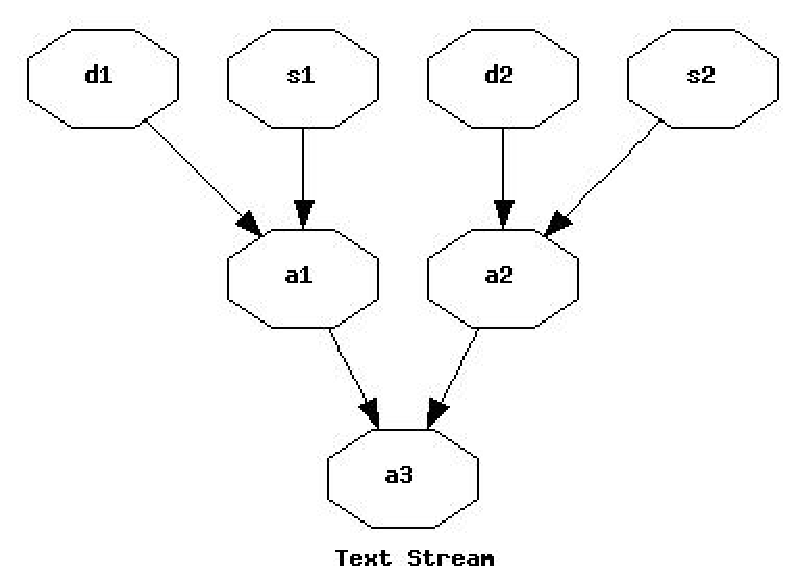
\includegraphics[width=4in]{pedfromstring.eps}
    \caption{Pedigree loaded from a string}
    \label{fig:ped-from-string}
  \end{center}
\end{figure}
\section{Contribute a HOWTO}
\label{sec:howto-contribute}
\index{how do I!contribute a HOWTO}
Users are invited to contribute HOWTOs demonstrating how to solve problems they've found interesting.  In order for such HOWTOs to be considered for inclusion in this manual they must be licensed under the GNU Free Documentation License version 1.2 or later (\url{http://www.gnu.org/copyleft/fdl.html}).  Authorship will be acknowledged, and copyright will remain with the author of the HOWTO.

\chapter{Graphics}
\label{cha:graphics}
\begin{quote}
If I could say it in words there would be no reason to paint. --- Edward Hopper
\end{quote}
\section{PyPedal Graphics}
\label{sec:graphics-overview}
\index{graphics}
\PyPedal{} is capable of producing graphics from information contained in a pedigree, including pedigree drawings, line graphs of changes in genetic diversity over time, and visualizations of numerator relationship matrices.  These graphics are non-interactive: output images are created and written to output files.  A separate program must be used to view and/or print the image; web browsers make reasonably good viewers for a small number of images.  If you are creating and viewing large numbers of images you may want to obtain an image management package for your platform.  Default and supported file formats for each of the graphics routines are presented in Table \ref{tbl:pypedal-graphics-formats}.
\begin{center}
    \tablecaption{Default graphics formats.}
    \tablefirsthead{\hline Routine & Default Format & Supported Formats \\ \hline}
    \tablehead{\hline Routine & Default Format & Supported Formats \\ \hline}
    \tabletail{\hline \multicolumn{3}{l}{\small\sl continued on next page} \\ \hline}
    \tablelasttail{\hline}
    \label{tbl:pypedal-graphics-formats}
    \begin{xtabular}{llp{2in}}
	draw\_pedigree & JPG & JPG, PNG, PS \\
	new\_draw\_pedigree & JPG & JPG, PNG, PS \\
	pcolor\_matrix\_pylab & PNG & PNG only \\
	plot\_founders\_by\_year & PNG & PNG only \\
	plot\_founders\_pct\_by\_year & PNG & PNG only \\
	plot\_line\_xy & PNG & PNG only \\
	rmuller\_pcolor\_matrix\_pil & PNG & PNG only \\
	rmuller\_spy\_matrix\_pil & PNG & PNG only \\
	spy\_matrix\_pylab & PNG & PNG only \\
    \end{xtabular}
\end{center}
\subsection{Drawing Pedigrees}
\label{sec:graphics-drawing-pedigrees}
\index{graphics!drawing pedigrees}
The pedigree from Figure 2 in Boichard et al. \citeyear{ref352} is shown in Figure \ref{fig:boichard2-pedigree}, and shows males enclosed in rectangles and females in ovals.  Figure \ref{fig:new-ids2-pedigree-basic} shows a pedigree in which strings are used for animal IDs; animal are enclosed in ovals because sexes were not specified in the pedigree file and the \member{set\_sexes} option was not specified.  A more complex German Shepherd pedigree is presented in Figure \ref{fig:doug-pedigree-basic}; the code used to create this pedigree is:
\begin{verbatim}
pyp_graphics.draw_pedigree(example, gfilename='doug_p_rl_notitle', gname=1,
    gdirec='RL', gfontsize=12)
\end{verbatim}
\begin{figure}
  \begin{center}
    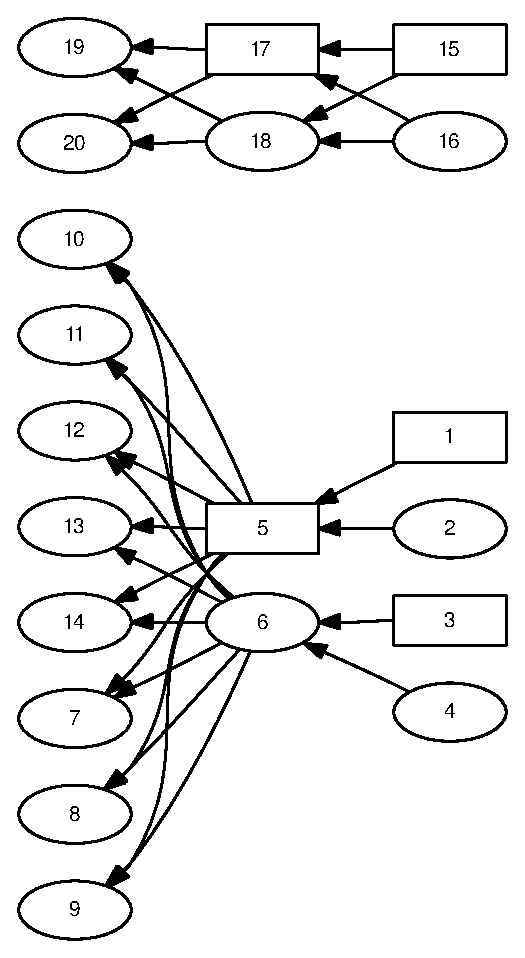
\includegraphics[width=4in]{boichard2Pedigree.eps}
    \caption{Pedigree 2 from Boichard et al. (1997)}
    \label{fig:boichard2-pedigree}
  \end{center}
\end{figure}
\begin{figure}
  \begin{center}
    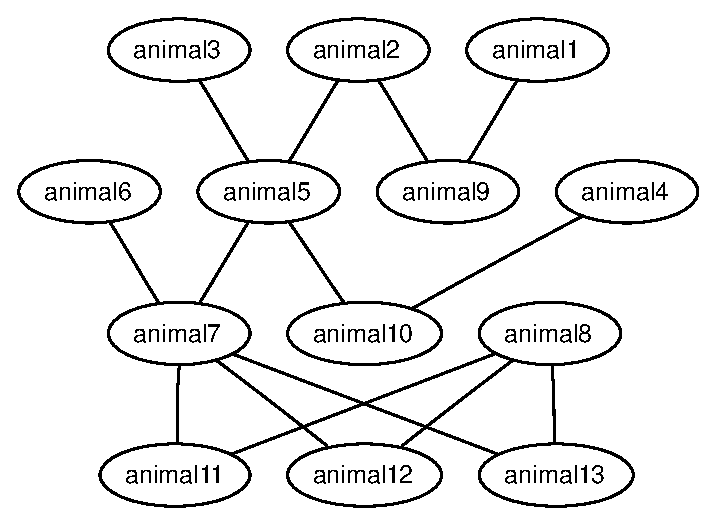
\includegraphics[width=3in]{BoichardPedigreeBasic.eps}
    \caption{A pedigree with strings as animal IDs}
    \label{fig:new-ids2-pedigree-basic}
  \end{center}
\end{figure}
\begin{figure}
  \begin{center}
    \includegraphics[width=4in]{dougPRlNotitle.eps}
    \caption{German Shepherd pedigree}
    \label{fig:doug-pedigree-basic}
  \end{center}
\end{figure}
The resulting graphic is written to doug\_p\_rl\_notitle.jpg; note from Table \ref{tbl:pypedal-graphics-formats} that the default file format for \function{draw\_pedigree()} is \textbf{JPG} rather than \textbf{PNG}, as is the case for the other graphics routines.  To get a PNG simply pass the argument \var{gformat='png'} to \function{draw\_pedigree()}.  For details on the options taken by \function{draw\_pedigree()} please refer to the API documentation (Section \ref{sec:pyp-graphics-draw-pedigree}). \function{draw\_pedigree()} uses rectangles to indicates known males, circles to indicate known females, and octagons to indicate animals of unknown sex.

Pedigrees can also be colored using the \function{color\_pedigree()} function in the \module{pyp\_jbc} module. At present, animals are shaded either by the number of sons produced or by the total number of descendants. The five-generation pedigree of the Newfoundland dog King von der D\"{u}ssel is presented in Figure \ref{fig:newfoundland-colored-pedigree} (\url{http://www.newfoundlanddog-database.net/en/ahnen.php?num=0000025330}, data used with permission), and the nodes are shaded based on number of descendants.
\begin{figure}
  \begin{center}
    \includegraphics[width=4in]{newfoundland.eps}
    \caption{Newfoundland colored pedigree}
    \label{fig:newfoundland-colored-pedigree}
  \end{center}
\end{figure}

\fixme{Windows users should set the \var{drawers} keyword to 'old' when calling \function{color\_pedigree()}. This will call \function{draw\_colored\_pedigree()} rather than \function{new\_draw\_colored\_pedigree()}. The latter requires that PyGraphviz library be installed and there is not yet an easy way to install it on Windows.}
\subsection{Drawing Line Graphs}\label{sec:graphics-drawing-line-graphs}\index{graphics!drawing line graphs}
The \texttt{plot\_line\_xy()} routine provides a convenient tool for creating two-dimensional line graphs.  Figure \ref{fig:ayrshire-coi-graph} shows the plot of inbreeding by birth year for the US Ayrshire cattle population.  The plot is produced by the call:
\begin{verbatim}
pyp_db.loadPedigreeTable(ay)
coi_by_year = pyp_reports.meanMetricBy(ay,metric='fa',byvar='by')
cby = coi_by_year
del(cby[1900])
pyp_graphics.plot_line_xy(coi_by_year, gfilename='ay_coi_by_year',
    gtitle='Inbreeding coefficients for Ayrshire cows', gxlabel='Birth year',
    gylabel='Coefficient of inbreeding')
\end{verbatim}
\begin{figure}
  \begin{center}
    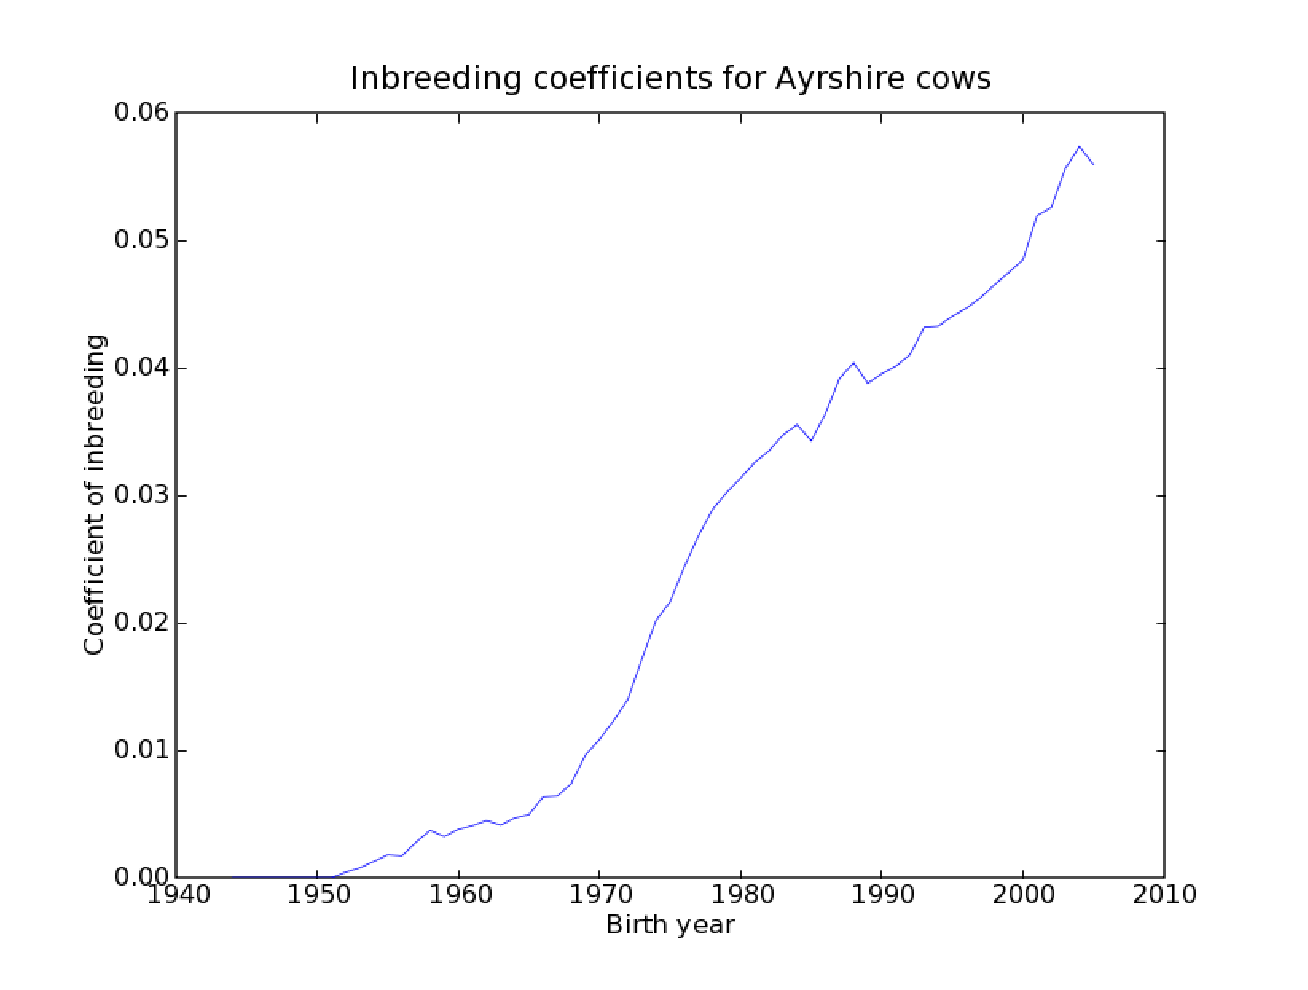
\includegraphics[width=4in]{ayCoiByYear.eps}
    \caption{Average inbreeding by birth year for the US Ayrshire cattle population}
    \label{fig:ayrshire-coi-graph}
  \end{center}
\end{figure}
The code above uses \function{pyp_reports.meanMetricBy()} (see \ref{sec:pyp-reports-mean-metric-by}) to populate \var{coi_by_year}; the keys in \var{coi\_by\_year} are plotted in the x-axis, and the values are plotted on the y-axis.  The default birth year, 1900, was deleted from the dictionary before the plot was drawn because leaving the default birthyear in the plot was distracting and somewhat misleading.  The only restriction that you have to observe is that the value plotted on the y-ais has to be a numeric quantity.

If you need more complicated plots than are produced by \function{plot\_line\_xy()} you can write a new plotting function (Chapter \ref{cha:newfeatures}) that uses the tools in matplotlib (\url{http://matplotlib.sourceforge.net/}). For complete details on the options taken by \function{plot\_line\_xy{}} please refer to the API documentation (\ref{sec:pyp-graphics-plot-line-xy}).
\subsection{Visualizing Numerator Relationship Matrices}
\label{sec:graphics-visualizing-nrm}
\index{graphics!visualizing relationship matrices}
Two routines are provided for visualization of numerator relationship matrices (NRM), \function{rmuller_pcolor_matrix_pil()} and \function{rmuller_spy_matrix_pil()}.

As an example, we will consider the NRM for the pedigree in Figure \ref{fig:boichard2-pedigree}.  The matrix is square and symmetric; the diagonal values correspond to $1+f_a$, where $f_a$ is an animal's coefficient of inbreeding; animals with a diagonal element $>1$ are inbred.
\[
    \scriptsize
    \left[ \begin{array}{llllllllllllllllllll}
        1. & 0. & 0. & 0. & 0.5 & 0. & 0.25 & 0.25 & 0.25 & 0.25 & 0.25 & 0.25 & 0.25 & 0.25 & 0. & 0. & 0. & 0. & 0. & 0. \\
        0. & 1. & 0. & 0. & 0.5 & 0. & 0.25 & 0.25 & 0.25 & 0.25 & 0.25 & 0.25 & 0.25 & 0.25 & 0. & 0. & 0. & 0. & 0. & 0. \\
        0. & 0. & 1. & 0. & 0.  & 0.5 & 0.25 & 0.25 & 0.25 & 0.25 & 0.25 & 0.25 & 0.25 & 0.25 & 0. & 0. & 0. & 0. & 0. & 0. \\
        0. & 0. & 0. & 1. & 0. & 0.5 & 0.25 & 0.25 & 0.25 & 0.25 & 0.25 & 0.25 & 0.25 & 0.25 & 0. & 0. & 0. & 0. & 0. & 0. \\
        0.5 & 0.5 & 0. & 0. & 1. & 0. & 0.5 & 0.5 & 0.5 & 0.5 & 0.5 & 0.5 & 0.5 & 0.5 & 0. & 0. & 0. & 0. & 0. & 0. \\
        0. & 0. & 0.5 & 0.5 & 0. & 1. & 0.5 & 0.5 & 0.5 & 0.5 & 0.5 & 0.5 & 0.5 & 0.5 & 0. & 0. & 0. & 0. & 0. & 0. \\
        0.25 & 0.25 & 0.25 & 0.25 & 0.5 & 0.5 & 1. & 0.5 & 0.5 & 0.5 & 0.5 & 0.5 & 0.5 & 0.5 & 0. & 0. & 0. & 0. & 0. & 0. \\
        0.25 & 0.25 & 0.25 & 0.25 & 0.5 & 0.5 & 0.5 & 1. & 0.5 & 0.5 & 0.5 & 0.5 & 0.5 & 0.5 & 0. & 0. & 0. & 0. & 0. & 0. \\
        0.25 & 0.25 & 0.25 & 0.25 & 0.5 & 0.5 & 0.5 & 0.5 & 1. & 0.5 & 0.5 & 0.5 & 0.5 & 0.5 & 0. & 0. & 0. & 0. & 0. & 0. \\
        0.25 & 0.25 & 0.25 & 0.25 & 0.5 & 0.5 & 0.5 & 0.5 & 0.5 & 1. & 0.5 & 0.5 & 0.5 & 0.5 & 0. & 0. & 0. & 0. & 0. & 0. \\
        0.25 & 0.25 & 0.25 & 0.25 & 0.5 & 0.5 & 0.5 & 0.5 & 0.5 & 0.5 & 1. & 0.5 & 0.5 & 0.5 & 0. & 0. & 0. & 0. & 0. & 0. \\
        0.25 & 0.25 & 0.25 & 0.25 & 0.5 & 0.5 & 0.5 & 0.5 & 0.5 & 0.5 & 0.5 & 1. & 0.5 & 0.5 & 0. & 0. & 0. & 0. & 0. & 0. \\
        0.25 & 0.25 & 0.25 & 0.25 & 0.5 & 0.5 & 0.5 & 0.5 & 0.5 & 0.5 & 0.5 & 0.5 & 1. & 0.5 & 0. & 0. & 0. & 0. & 0. & 0. \\
        0.25 & 0.25 & 0.25 & 0.25 & 0.5 & 0.5 & 0.5 & 0.5 & 0.5 & 0.5 & 0.5 & 0.5 & 0.5 & 1. & 0. & 0. & 0. & 0. & 0. & 0. \\
        0. & 0. & 0. & 0. & 0. & 0. & 0. & 0. & 0. & 0. & 0. & 0. & 0. & 0. & 1. & 0. & 0.5 & 0.5 & 0.5 & 0.5 \\
        0. & 0. & 0. & 0. & 0. & 0. & 0. & 0. & 0. & 0. & 0. & 0. & 0. & 0. & 0. & 1. & 0.5 & 0.5 & 0.5 & 0.5 \\
        0. & 0. & 0. & 0. & 0. & 0. & 0. & 0. & 0. & 0. & 0. & 0. & 0. & 0. & 0.5 & 0.5 & 1. & 0.5 & 0.75 & 0.75 \\
        0. & 0. & 0. & 0. & 0. & 0. & 0. & 0. & 0. & 0. & 0. & 0. & 0. & 0. & 0.5 & 0.5 & 0.5 & 1. & 0.75 & 0.75 \\
        0. & 0. & 0. & 0. & 0. & 0. & 0. & 0. & 0. & 0. & 0. & 0. & 0. & 0. & 0.5 & 0.5 & 0.75 & 0.75 & 1.25 & 0.75 \\
        0. & 0. & 0. & 0. & 0. & 0. & 0. & 0. & 0. & 0. & 0. & 0. & 0. & 0. & 0.5 & 0.5 & 0.75 & 0.75 & 0.75 & 1.25
    \end{array} \right]
    \normalsize
\]
Note that the array only contains six distinct values: 0., 0.25, 0.5, 0.75, 1.0, and 1.25.  These six values will be used to create the color map used by \function{rmuller_pcolor_matrix_pil()}.

\function{rmuller_pcolor_matrix_pil()} produces pseudocolor plots from NRM.  A pseudocolor plot is an array of cells that are colored based on the values the corresponding cells in the NRM. The minimum and maximum values in the NRM are assigned the first and last colors in the colormap; other cells are colored by mapping their values to colormap elements.  In the example above, the minimum value is 0.0 and the maximum value is 1.0 (Figure \ref{fig:boichard2-pseudocolor}).  The two inbred animals in the population are easily identified as the yellow diagonal elements in the bottom-left corner of the matrix.
\begin{figure}[tb]
  \begin{center}
    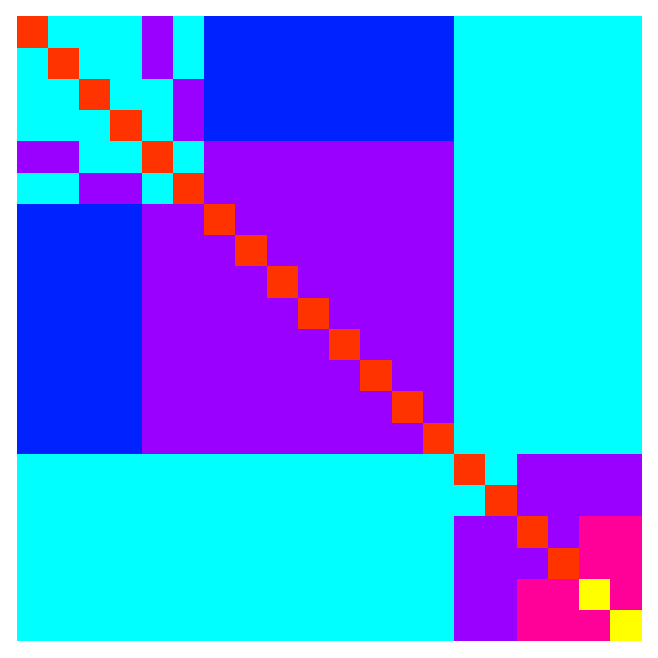
\includegraphics[width=3in]{boichard2Pcolor.eps}
    \caption{Pseudocolored NRM from the Boichard et al. (1997) pedigree}
    \label{fig:boichard2-pseudocolor}
  \end{center}
\end{figure}
\function{rmuller_spy_matrix_pil()} is similar to \function{rmuller_pcolor_matrix_pil()}, but it is used to visualize the sparsity of a matrix.  Cells are either filled, indicating that the value is non-zero, or not filled, indicating that the cell's value is zero.  In Figure \ref{fig:boichard2-sparsity} it is easy to see the two separate families in the pedigree.
\begin{figure}[tb]
  \begin{center}
    
\includegraphics[width=3in]{boichard2Spy.eps}
    \caption{Sparsity of the NRM from the Boichard et al. (1997) pedigree}
    \label{fig:boichard2-sparsity}
  \end{center}
\end{figure}
\chapter{Report Generation}
\label{cha:reports}
\begin{quote}
If we spoke a different language, we would perceive a somewhat different world. --- Ludwig Wittgenstein
\end{quote}
\section{Overview}\label{sec:reports-overview}\index{report generation}
An overview of the report generation tools in \PyPedal{} is provided in this chapter.  The creation of a new, custom report is demonstrated.

\PyPedal{} has a framework in place to support basic report generation.  This franework consists of two components: a database access module, \module{pyp\_db} (Section \ref{sec:pyp-db}), and a reporting module, \module{pyp\_reports} (Section \ref{sec:pyp-reports}).  The SQLite 3 database engine (\url{http://www.sqlite.org/}) is used to store data and generate reports.  The ReportLab extension to Python (\url{http://www.reportlab.org/}) allows users to create reports in the Adobe Portable Document Format (PDF).  As a result, there are two types of reports that can be produced: internal summaries that can be fed to other \PyPedal{} routines (e.g. the report produced by \function{pyp\_reports.meanMetricBy()} can be passed to \function{pyp\_graphics.plot\_line\_xy()} to produce a plot) and printed reports in PDF format.  When referencing the \module{pyp\_reports} API note that the convention used in \PyPedal{} is that procedures which produce PDFs are prepended with 'pdf'.  Sections \ref{sec:reports-custom-internal-reports} and \ref{sec:reports-custom-printed-reports} demonstrate how to create new or custom reports.  \module{pyp\_reports} was added to \PyPedal{} with the intention that end-users develop their own custom reports using \function{pyp\_reports.meanMetricBy()} as a template.  More material on adding new functionality to \PyPedal{} can be found in Chapter \ref{cha:newfeatures}.

Column names, data types, and descriptions of contents for pedigree tables are presented in Table
\ref{tbl:reports-db-column-names}.  The \constant{metric\_to\_column} and \constant{byvar\_to\_column} dictionaries in
\module{pyp\_db} are used to convert between convenient mnemonics and database column names.  You may need to refer
to Table \ref{tbl:reports-db-column-names} for unmapped column names when writing custom reports.  If you happen
to view a table scheme using the \textbf{sqlite3} command-line utility you will notice that the columns are ordered
differently in the database than they are in the table; the table has been alphabetized for easy reference.
\begin{center}
    \tablecaption{Columns in pedigree database tables.}
    \tablefirsthead{\hline Name & Type & Note(s) \\ \hline}
    \tablehead{\hline Name & Type & Note(s) \\ \hline}
    \tabletail{\hline \multicolumn{3}{l}{\small\sl continued on next page} \\ \hline}
    \tablelasttail{\hline}
    \label{tbl:reports-db-column-names}
    \begin{xtabular}{llp{2.5in}}
	age           &   real          &  Age of animal \\
	alive         &   char(1)       &  Animal's mortality status \\
	ancestor      &   char(1)       &  Ancestor status \\
	animalID      &   integer       &  \textbf{Must be unique!} \\
	animalName    &   varchar(128)  &  Animal name \\
	birthyear     &   integer       &  Birth year \\
	breed         &   text          &  Breed \\
	coi           &   real          &  Coefficient of inbreeding \\
	damID         &   integer       &  Dam's ID \\
	founder       &   char(1)       &  Founder status \\
	gencoeff      &   real          &  Pattie's generation coefficient \\
	generation    &   real          &  Generation \\
	herd          &   integer       &  Herd ID \\
	infGeneration &   real          &  Inferred generation \\
	num\_daus     &   integer       &  Number of daughters \\
	num\_sons     &   integer       &  Number of sons \\
	num\_unk      &   integer       &  Offspring of unknown sex \\
	originalHerd  &   varchar(128)  &  Original herd ID \\
	originalID    &   text          &  Animal's original ID \\
	pedgreeComp   &   real          &  Pedigree completeness \\
	renumberedID  &   integer       &  Animal's renumbered ID \\
	sex           &   char(1)       &  Sex of animal \\
	sireID        &   integer       &  Sire's ID \\
    \end{xtabular}
\end{center}

\subsection{Three Generation Pedigrees}
\label{sec:reports-three-gen-peds}
\index{report generation!three generation pedigrees}
A report for producing three-generation pedigrees, \function{pdf3GenPed()}, is included in the \module{pyp_reports} module. The sample output shown in Figure \ref{fig:reports-three-gen-ped} contains output for one animal. However, if \function{pdf3GenPed()} is passed a list of animal IDs the resulting PDF will contain a pedigree for each animal that can be printed as a booklet. See Section \ref{sec:pyp-reports-pdf-three-gen-ped} for usage details.
\begin{figure}
  \begin{center}
    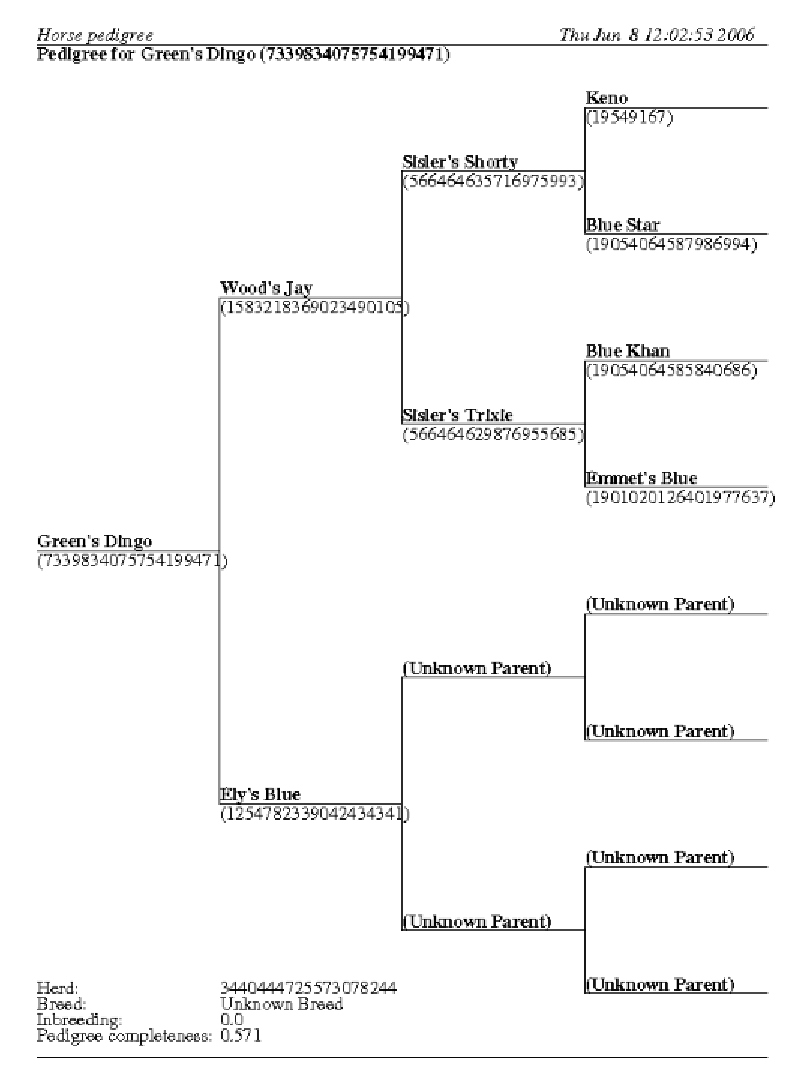
\includegraphics[width=6in]{greensDingoPedigree.eps}
    \caption{Example of a printed three generation pedigree.}
    \label{fig:reports-three-gen-ped}
  \end{center}
\end{figure}

\section{Creating a Custom Internal Report}
\label{sec:reports-custom-internal-reports}
\index{report generation!creating custom internal reports}
Internal reports \index{internal reports} typically aggregate data such that the result can be handed off to another \PyPedal{} routine for further processing.   To do this, the pedigree is loaded into a table in an SQLite database against which queries are made.  This is faster and more flexible than writing reporting routines that loop over the pedigree to construct reports, but it does require some knowledge of the Structured Query Language (SQL; \url{http://www.sql.org/}).  The canonical example of this kind of report is the passing of the dictionary returned by \function{pyp\_reports.meanMetricBy()} to \function{pyp\_graphics.plot\_line\_xy()} (see \ref{sec:graphics-drawing-pedigrees}).  That approach is outlined in code below.
\begin{verbatim}
def inbreedingByYear(pedobj):
    curs = pyp_db.getCursor(pedobj.kw['database_name'])

    # Check and see if the pedigree has already been loaded.  If not, do it.
    if not pyp_db.tableExists(pedobj.kw['database_name'], pedobj.kw['dbtable_name']):
        pyp_db.loadPedigreeTable(pedobj)

    MYQUERY = "SELECT birthyear, pyp_mean(coi) FROM %s GROUP BY birthyear \
        ORDER BY birthyear ASC" % (pedobj.kw['dbtable_name'])
    curs.execute(MYQUERY)
    myresult = curs.fetchall()
    result_dict = {}
    for _mr in myresult:
        _level, _mean = _mr
        result_dict[_level] = _mean
    return result_dict
\end{verbatim}
You should always check to see if your pedigree has been loaded into the database before you try and make queries against the pedigree table or your program may crash.  \function{inbreedingByYear()} returns a dictionary containing average coefficients of inbreeding keyed to birth years.  The query result, \var{myresult}, is a list of tuples; each tuple in the list
corresponds to one row in an SQL resultset. The tuples in \var{myresult} are unpacked into temporary variables that are then stored in the dictionary, \var{result\_dict} (for information on tuples see the Python Tutorial (\url{http://www.python.org/doc/tut/node7.html#SECTION007300000000000000000}).  If the resultset is empty, \var{result\_dict} will also be empty.  As long as you can write a valid SQL query for the report you'd like to assemble, there is no limitation on the reports that can be prepared by \PyPedal{}.
\section{Creating a Custom Printed Report}
\label{sec:reports-custom-printed-reports}
\index{report generation!creating custom printed reports}
If you are interested in custom printed reports you should begin by opening the file \texttt{pyp\_reports.py} and reading
through the code for the \function{pdfPedigreeMetadata()} report.  It has been heavily commented so that it can be used as
a template for developing other reports.  ReportLab provides fairly low-level tools that you can use to assemble
documents.  The basic idea is that you create a canvas on which your image will be drawn.  You then create text objects and
draw them on the canvas.  When your report is assembled you save the canvas on which it's drawn to a file.  \PyPedal{} provides
a few convenience functions for such commonly-used layouts as title pages and page "frames".  In the following sections of code I will discuss the creation of a \function{pdfInbreedingByYear()} printed report to accompany the
\function{inbreedingByYear()} internal report written in Section \ref{sec:reports-custom-internal-reports}.  First, we import ReportLab and check to see if the user provided an output file name.  If they didn't, revert to a default.
\begin{verbatim}
def pdfInbreedingByYear(pedobj,results,titlepage=0,reporttitle='',reportauthor='', \
    reportfile=''):
    import reportlab
    if reportfile == '':
        _pdfOutfile = '%s_inbreeding_by_year.pdf' % ( pedobj.kw['default_report'] )
    else:
        _pdfOutfile = reportfile
\end{verbatim}
Next call \function{\_pdfInitialize()}, which returns a dictionary of settings, mostly related to page size and
margin locations, that is used throughout the routine.  \function{\_pdfInitialize()} uses the \member{paper\_size} keyword
in the pedigree's options dictionary, which is either `letter' or `A4', and the \member{default\_unit}, which is either
`inch' or `cm' to populate the returned structure.  This should allow users to move between paper sizes without little
or no work.  Once the PDF settings have been computed we instantiate a canvas object on which to draw.
\begin{verbatim}
_pdfSettings = _pdfInitialize(pedobj)
canv = canvas.Canvas(_pdfOutfile, invariant=1)
canv.setPageCompression(1)
\end{verbatim}
There is a hook in the code to toggle cover pages on and off.  It is arguably rather pointless to put a cover page on a one-page document, but all TPS reports require new coversheets.  The call to \function{\_pdfDrawPageFrame()} frames the page with a header and footer that includes the pedigree name, date and time the report was created, and the page number.
\begin{verbatim}
if titlepage:
    if reporttitle == '':
        reporttitle = 'meanMetricBy Report for Pedigree\n%s' \
            % (pedobj.kw['pedname'])
    _pdfCreateTitlePage(canv, _pdfSettings, reporttitle, reportauthor)
_pdfDrawPageFrame(canv, _pdfSettings)
\end{verbatim}
The largest chunk of code in \function{pdfInbreedingByYear()} is dedicated to looping over the input dictionary, \var{results}, and writing its contents to text objects.  If you want to change the typeface for the rendered text, you need to make the appropriate changes to all calls to \texttt{canv.setFont("Times-Bold", 12)}.  The ReportLab documentation includes a discussion of available typefaces.
\begin{verbatim}
canv.setFont("Times-Bold", 12)
tx = canv.beginText( _pdfSettings['_pdfCalcs']['_left_margin'],
    _pdfSettings['_pdfCalcs']['_top_margin'] - 0.5 * \
        _pdfSettings['_pdfCalcs']['_unit'] )
\end{verbatim}
Every printed report will have a section of code in which the input is processed and written to text objects. In this case, the code loops over the key-and-value pairs in \var{results}, determines the width of the key, and creates a string with the proper spacing between the key and its value.  That string is then written to a \method{tx.textLine()} object.
\begin{verbatim}
# This is where the actual content is written to a text object that
# will be displayed on a canvas.
for _k, _v in results.iteritems():
    if len(str(_k)) <= 14:
        _line = '\t%s:\t\t%s' % (_k, _v)
    else:
        _line = '\t%s:\t%s' % (_k, _v)
    tx.textLine(_line)
\end{verbatim}
ReportLab's text objects do not automatically paginate themselves.  If you write, say, ten pages of material to a text object and render it without manually paginating the object you're going to get a single page of chopped-off text.  The following section of code is where the actual pagination occurs, so careful cutting-and-pasting should make pagination seamless.
\begin{verbatim}
    # Paginate the document if the contents of a textLine are longer than one page.
    if tx.getY() < _pdfSettings['_pdfCalcs']['_bottom_margin'] + \
        0.5 * _pdfSettings['_pdfCalcs']['_unit']:
        canv.drawText(tx)
        canv.showPage()
        _pdfDrawPageFrame(canv, _pdfSettings)
        canv.setFont('Times-Roman', 12)
        tx = canv.beginText( _pdfSettings['_pdfCalcs']['_left_margin'],
            _pdfSettings['_pdfCalcs']['_top_margin'] -
            0.5 * _pdfSettings['_pdfCalcs']['_unit'] )
\end{verbatim}
Once we're done writing our text to text objects we need to draw the text object on the canvas and make the canvas visible.  If you omit this step, perhaps because of the kind of horrible cutting-and-pasting accident to which I am prone, your PDF will not be written to a file.
\begin{verbatim}
if tx:
    canv.drawText(tx)
    canv.showPage()
canv.save()
\end{verbatim}
While \PyPedal{} does not yet have any standard reports that include graphics, ReportLab does support adding graphics, such as a pedigree drawing, to a canvas.  Interested readers should refer to the ReportLab documentation.
\chapter{Implementing New Features}
\label{cha:newfeatures}
\begin{quote}
First, solve the problem. Then, write the code. --- John Johnson
\end{quote}
\section{Overview}\label{sec:newfeatures-overview}\index{new features}
In this chapter, an example of wil be provided of how to extend \PyPedal{} by creating a user-defined routine.  New routines may implement a new measure of genetic diversity, extend the graphics module, add a new report, or group a series of actions into a single convenient routine.

One of the appealing features of \PyPedal{} is its easy extensibility.  In this section, we will demonstrate how to add a
user-written module to \PyPedal{}.  The file \texttt{pyp\_template.py} that is distributed with \PyPedal{} is a
skeleton that can be used to help you get started writing your custom module(s).  You should also look at the source
code of the standard modules, particularly if there is already a routine that does something similar to what you would
like to do, to see if you can jump-start your project by reusing code.
\subsection{Defining the Problem}
\label{sec:newfeatures-overview-problem}
\index{new features!defining the problem}
Before you open your editor and begin writing code you need to clearly define your problem.  Answering a few questions can
help you do this:
\begin{itemize}
\item What output do I want from my routine?
\item What calculations do I need to perform?
\item What input do I need to give my routine in order to perform those calculations?
\item Are there any \PyPedal{} routines that already do something similar?
\end{itemize}
The last question is as important as the others --- if there is already a \PyPedal{} routine that does similar calculations
you can use it as a starting point.  Code reuse is a great idea.

The problem that will motivate the rest of this section sounds very tricky, but is not really so bad because we are going to
reuse a lot of code.  I want to create a routine for drawing pedigrees that color nodes (animals) based on their importance as
measured by their connectedness to other animals in the pedigree.  After a brief review of the contents of the Module Template
in Section \ref{sec:newfeatures-template}, I will present a detailed solution to this problem in Section
\ref{sec:newfeatures-solving-the-problem}.
\section{Module Template}
\label{sec:newfeatures-template}
\index{new features!module template}
The file \file{pyp\_template.py} is a skeleton that can be used to get started writing a custom module.  The first thing you should do is save a copy of \file{pyp\_template.py} with your working module name; we will use the filename \file{pyp\_jbc.py} for the following example.  You should also fill-in the module header so that it contains your name, e-mail address, etc.  The version number of your module does not have to match that of the main \PyPedal{} distribution, and is only used as an aid to the programmer.
\index{new features!module template!header}
\begin{verbatim}
###############################################################################
# NAME: pyp_jbc.py
# VERSION: 1.0.0 (16NOVEMBER2005)
# AUTHOR: John B. Cole, PhD (jcole@aipl.arsusda.gov)
# LICENSE: LGPL
###############################################################################
# FUNCTIONS:
#     get_color_32()
#     color_pedigree()
#     draw_colored_pedigree()
###############################################################################
\end{verbatim}
The imports section of the template includes \code{import} statements for all of the standard \PyPedal{} modules.  There's
no harm in including all of them in your module, but it's good practice to include only the modules you need. You should
always include the \module{logging} module because it's needed for communicating with the log file.  For \module{pyp\_jbc}
I am including only the \module{pyp\_graphics}, \module{pyp\_network}, and \module{pyp\_utils} modules.
\index{new features!module template!imports}
\begin{verbatim}
##
# pyp_jbc provides tools for enhanced pedigree drawing.
##
import logging
from PyPedal import pyp_graphics
from PyPedal import pyp_network
from PyPedal import pyp_utils
\end{verbatim}
There is a very sketchy function prototype included in the template.  It is probably enough for you to get started if you have
a little experience programming in Python.  If you don't have any experience programming in Python you should be able to get
up-and-running with a little trial-and-error and some study of \PyPedal{} source.  You should always write a comment block similar to that attached to \function{yourFunctionName()} for each of your functions.  This comment block is recognized by PythonDoc, a tool for automatically generating program documentation.  Parameters are the inputs that you send to a function, return is a description of the function's output, and defreturn is the type of output that is returned, such as a list, dictionary, integer, or tuple.
\index{new features!module template!function prototype}
\begin{verbatim}
##
# yourFunctionName() <description of what function does>
# @param <parameter_name> <parameter description>
# @return <description of returned value(s)
# @defreturn <type of returned data, e.g., 'dictionary' or 'list'>
def yourFunctionName(pedobj):
    try:
        # Do something here
        logging.info('pyp_template/yourFunctionName() did something.')
        # return a value/dictionary/etc.
    except:
        logging.error('pyp_template/yourFunctionName() encountered a problem.')
        return 0
\end{verbatim}
\section{Solving the Problem}
\label{sec:newfeatures-solving-the-problem}
\index{new features!solving the problem}
The measure of connectedness I am going to use for coloring the pedigree is the proportion of animals in the pedigree that are descended from each animal in the pedigree.  In order to do this we need to do the following:
\begin{enumerate}
\item Compute the proportion of animals in the pedigree that are descended from each animal in the pedigree; the values will
be stored in a dictionary keyed by animal IDs.
\item Map the proportion of descendants from decimal values on the interval (0,1) to RGB triples.
\item Use the RGB triples to set the fill color for nodes.
\end{enumerate}
There is not an existing function for the first item, but there is a function in the \module{pyp\_network} module, \function{find_descendants()}, for identifying all of the descendants of an animal.  We can use the length of the list of descendants and the number of animals in the pedigree to calculate the proportion of animals in the pedigree descended from that animal.  The \function{color\_pedigree()} function creates a dictionary and loops over the pedigree to compute the proporions.  It also calls \function{draw\_colored\_pedigree()}, which is a modified version of \function{pyp\_graphics.draw\_pedigree()}, to draw the pedigree with colored nodes.
\begin{verbatim}
##
# color_pedigree() forms a graph object from a pedigree object and
# determines the proportion of animals in a pedigree that are
# descendants of each animal in the pedigree.  The results are used
# to feed draw_colored_pedigree().
# @param pedobj A PyPedal pedigree object.
# @return A 1 for success and a 0 for failure.
# @defreturn integer
def color_pedigree(pedobj):
    _pedgraph = pyp_network.ped_to_graph(pedobj)
    _dprop = {}
    # Walk the pedigree and compute proportion of animals in the
    # pedigree that are descended from each animal.
    for _p in pedobj.pedigree:
        _dcount = pyp_network.find_descendants(_pedgraph,_p.animalID,[])
        if len(_dcount) < 1:
            _dprop[_p.animalID] = 0.0
        else:
            _dprop[_p.animalID] = float(len(_dcount)) / \
                float(pedobj.metadata.num_records)
    del(_pedgraph)
    _gfilename = '%s_colored' % \
        (pyp_utils.string_to_table_name(pedobj.metadata.name))
    draw_colored_pedigree(pedobj, _dprop, gfilename=_gfilename,
        gtitle='Colored Pedigree', gorient='p', gname=1, gdirec='',
        gfontsize=12, garrow=0, gtitloc='b')
\end{verbatim}
\function{pyp\_graphics.draw\_pedigree()} was copied into \module{pyp\_jbc}, renamed to \function{draw\_colored\_pedigree()}, and modified to draw colored nodes.  Two basic changes were made to accomplish that: the function was altered to accept a dictionary of weights to be used for coloring, and code for actually coloring the nodes was written.  The first change was simply the addition of a new required parameter, \var{shading}, to the function header.  The second step required a little more work.  For each animal in the pedigree, the descendant proportion is looked-up in the shading dictionary, the proportion is passed to \function{get\_color\_32()} and converted into an RGB triple, and the \member{filled} and \member{color} attributes for the node representing that animal are set.  The hardest part of creating this routine was determining where changes should be made when modifying \function{pyp\_graphics.draw\_pedigree()}.
\begin{verbatim}
##
# draw_colored_pedigree() uses the pydot bindings to the graphviz library
# to produce a directed graph of your pedigree with paths of inheritance
# as edges and animals as nodes.  If there is more than one generation in
# the pedigree as determind by the 'gen' attributes of the animals in the
# pedigree, draw_pedigree() will use subgraphs to try and group animals in
# the same generation together in the drawing.  Nodes will be colored
# based on the number of outgoing connections (number of offspring).
# @param pedobj A PyPedal pedigree object.
# @param shading A dictionary mapping animal IDs to levels that will be
#                used to color nodes.
# ...
# @return A 1 for success and a 0 for failure.
# @defreturn integer
def draw_colored_pedigree(pedobj, shading, gfilename='pedigree', \
    gtitle='My_Pedigree', gformat='jpg', gsize='f', gdot='1', gorient='l', \
    gdirec='', gname=0, gfontsize=10, garrow=1, gtitloc='b', gtitjust='c'):

    from pyp_utils import string_to_table_name
    _gtitle = string_to_table_name(gtitle)
    ...
    # If we do not have any generations, we have to draw a less-nice graph.
    if len(gens) <= 1:
        for _m in pedobj.pedigree:
            ...
            _an_node = pydot.Node(_node_name)
            ...
            _color = get_color_32(shading[_m.animalID],0.0,1.0)
            _an_node.set_style('filled')
            _an_node.set_color(_color)
            ...
    # Otherwise we can draw a nice graph.
    ...
        ...
            for _m in pedobj.pedigree:
                ...
                _an_node = pydot.Node(_node_name)
                ...
                _color = get_color_32(shading[_m.animalID])
                _an_node.set_style('filled')
                _an_node.set_color(_color)
                ...
\end{verbatim}
The \function{get\_color\_32()} function is a modified version of \function{pyp\_graphics.rmuller\_get\_color()} that returns RGB triplets of the form \samp{\#1a2b3c}, which are required by the program that renders the graphs.  This is another example of how code reuse can reduce development time.
\begin{verbatim}
##
# get_color_32() Converts a float value to one of a continuous range of colors
# using recipe 9.10 from the Python Cookbook.
# @param a Float value to convert to a color.
# @param cmin Minimum value in array (0.0 by default).
# @param cmax Maximum value in array (1.0 by default).
# @return An RGB triplet.
# @defreturn integer
def get_color_32(a,cmin=0.0,cmax=1.0):
    try:
        a = float(a-cmin)/(cmax-cmin)
    except ZeroDivisionError:
        a=0.5 # cmax == cmin
    blue = min((max((4*(0.75-a),0.)),1.))
    red = min((max((4*(a-0.25),0.)),1.))
    green = min((max((4*math.fabs(a-0.5)-1.,0)),1.))
    _r = '%2x' % int(255*red)
    if _r[0] == ' ':
        _r = '0%s' % _r[1]
    _g = '%2x' % int(255*green)
    if _g[0] == ' ':
        _g = '0%s' % _g[1]
    _b = '%2x' % int(255*blue)
    if _b[0] == ' ':
        _b = '0%s' % _b[1]
    _triple = '#%s%s%s' % (_r,_g,_b)
    return _triple
\end{verbatim}
This change will probably be to rolled into \function{rmuller\_get\_color()} so that the form of the return triplet is user-selectable.

The program \file{new_jbc.py} demonstrates use of the new \function{pyp\_jbc.color\_pedigree()} routine:
\begin{verbatim}
options = {}
options['renumber'] = 1
options['sepchar'] = '\t'
options['missing_parent'] = 'animal0'

if __name__=='__main__':
    options['pedfile'] = 'new_ids2.ped'
    options['pedformat'] = 'ASD'
    options['pedname'] = 'Boichard Pedigree'
    example = pyp_newclasses.loadPedigree(options)
    pyp_jbc.color_pedigree(example)
\end{verbatim}
The resulting colorized pedigree can be seen in Figure \ref{fig:boichard2-pedigree-colorized}.  Each of the nodes is colored
according to the proportion of animals in the complete pedigree descended from a given animal.  Clearly there is still room
for improvement; for example, there is no key provided in the image so that you can see how colors map to proportions.  Implementation
of a key is left as an exercise for the reader.
\begin{figure}
  \begin{center}
    \includegraphics[width=6in]{BoichardPedigreeColored.eps}
    \caption{Colorized version of the pedigree in Figure \ref{fig:new-ids2-pedigree-basic}}
    \label{fig:boichard2-pedigree-colorized}
  \end{center}
\end{figure}
\section{Contributing Code to PyPedal}
\label{sec:newfeatures-overview-contributing-code}
\index{new features!contributing code}
If you would like to contribute your code back to \PyPedal{} please note that it must be licensed under version 2.1 or any
later version of the GNU Lesser General Public License.  The GNU LGPL has all of the restrictions of the GPL except that you
may use the code at compile time without the derivative work becoming a GPL work. This allows the use of the code in
proprietary works.  You must also complete and return the joint copyright assignment form distributed as
\texttt{pypedal\_copyright\_assignment.pdf} before any contributions can be accepted and merged into the development tree.

Contributors are asked to document their code using the documentation comments recognized by PythonDoc 2.0 or later
(\url{http://effbot.org/zone/pythondoc.htm}).  PythonDoc is used to generates API documentation in HTML and other formats
based on descriptions in Python source files.  You are also strongly encouraged to provide example programs abd datasets
with any code submissions.
\chapter{Glossary}
\label{cha:glossary}
\begin{quote}
Just as birds have wings, man has language. --- George Henry Lewes
\end{quote}
This chapter provides a glossary of terms.\footnote{Please let me know of any additions to this list which you feel would be helpful.}
\begin{description}
\item[ancestor loss coefficient] See: pedigree completeness.
\item[coefficient of ancestral inbreeding] The probability that an individual jas inherited an allele that has undergone inbreeding in the past at least once.
\item[coefficient of inbreeding] Probability that two alleles selected at random are identical by descent.
\item[coefficient of partial inbreeding] The probability that the alleles at an arbitrary locus in an individual are identitical-by-descent, and that the alleles were derived from an allele in a particular founder.
\item[coefficient of relationship] Proportion of genes that two individuals share on average.
\item[effective ancestor number] The number of equally-contributing ancestors, not necessarily founders, needed to produce a population with the heterozygosity of the studied population \cite{ref352}.
\item[effective founder number] The number of equally-contributing founders needed to produce a population with the heterozygosity of the studied population \cite{ref640}.
\item[effective population size] The effective population size is the size of an ideal population that would lose heterozygosity at a rate equal to that of the studied population \cite{ref91}.
\item[founder] An animal with unknown parents that is assumed to be unrelated to all other founders.
\item[internal report] A \PyPedal() report that is intended for use by other \PyPedal() procedures, such as plotting
routines, and not for printing.
\item[numerator relationship matrix] Matrix of additive genetic covariances among the animals in a population.
\item[pedigree] A \PyPedal{} pedigree consists of a Python list containing instances of \PyPedal{} \method{NewAnimal()} objects.
\item[pedigree completeness] The proportion of known pedigree information for an arbitrary number of generations.
\item[renumbering] Many calculations require that the animals in a pedigree be ordered from oldest to youngest, with sires and dams preceding offspring, and renumbered  starting with 1.  This is a computational necessity, and results in an animal's ID (\texttt{animalID}) being changed to reflect that animal's order in the pedigree.  All animals have their original IDs stored in their \texttt{originalName} attribute.
\item[reordering] The process of arranging animals in a pedigree so that parents appear before their offspring; this is a necessary step in renumbering a pedigree.
\end{description}
\appendix
\addcontentsline{toc}{chapter}{Appendices}
\chapter{Example Programs}\label{cha:example-programs}\index{example programs}
\begin{quote}
 Either I've invented a whole new logic or, ahem, I'm not playing with a full deck. --- Philip K. Dick
\end{quote}

A number of example programs are distributed with \PyPedal{}. Table \ref{tbl:examples-program-list} provides the name of each file, the configuration and pedigree files used by those programs, and a brief description of the concepts and techniques presented.
\begin{center}
    \tablecaption{Example programs distributed with \PyPedal{}.}
    \tablefirsthead{\hline Program Name & Configuration File & Pedigree File & Description \\ \hline}
    \tablehead{\hline Program Name & Configuration File & Pedigree File & Description \\ \hline}
    \tabletail{\hline \multicolumn{4}{l}{\small\sl continued on next page} \\ \hline}
    \tablelasttail{\hline}
    \label{tbl:examples-program-list}
    \begin{xtabular}{l|p{1in}|p{1in}|p{3in}}
    new\_amatrix.py & new\_amatrix.ini & new\_amatrix.ped & Create, save, load, and view information about NewAMatrix objects \\
    new\_classes.py & new\_classes.ini & boichard2.ped & ??? \\
    new\_db.py & new\_db.ini & hartlandclark.ped & Loading a pedigree into SQLite and creating a report of mean inbreeeding by birth year \\
    new\_decompose.py & new\_decompose.ini & new_decompose.ped & Use of numerator relationship matrix decomposition subroutines in \module{pyp_nrm} \\
    new\_doug.py & new\_doug.ini & doug.ped & Reading a pedigree in which names are strings, drawing pedigrees \\
    new\_format.py & new\_format.ini & boichard2a.ped & Reading a pedigree using the `skip column' format code (Z), printing pedigree metadata \\
    new\_graphics.py & new\_graphics.ini & boichard2.ped & Use of a number of routines from \module{pyp_graphics} \\
    new\_hartl.py & new\_hartl.ini & hartlandclark.ped & Demonstrates use of \function{pyp_graphics.draw_pedigree()} \\
    new\_ids.py & new\_ids.ini & new\_ids2.ped & Demonstrates reading tab-delimited files, using strings as animal IDs, overriding the default missing parent code, printing animal records \\
    new\_inbreeding.py & new\_inbreeding.ini & new\_renumbering.ped & Calculating coefficients of inbreeding \\
    new\_inbreeding2.py & new\_inbreeding2.ini, new\_inbreeding2multiple.ini & new\_renumbering.ped, horse.ped & Advanced .ini file techniques, computations on extremely inbred animals, calculation of summary statistics for coefficients of relationship \\
    new\_jbc.py & new\_jbc.ini & new\_ids2.ped & Using \function{pyp_jbc.color_pedigree()} to produce a weighted, colored pedigree \\
    new\_lacy.py & new\_lacy.ini, new\_format.ini & new\_lacy.ped, boichard2a.ped & Calculating effective ancestor and founder numbers \\
    new\_methods.py & new\_format.ini & boichard2a.ped & Use of \function{pyp_metrics.related\_animals()} and \function{pyp_metrics.common\_ancestors()} \\
    new\_networkx.py & new\_networkx.ini & generations.ped & Use of [algebraic] graph functions \\
    new\_options.py & new\_options.ini & new\_lacy.ped & Use of the configuration files \\
    new\_renumbering.py & new\_renumbering.ini & new\_renumbering.ped & Renumbering a pedigree, calculating inbreeding, pedigree drawing \\
    new\_reporting.py & new\_reporting.ini & new\_renumbering.ped & Use of reporting functions \\
    new\_simulate.py & new\_simulate.ini & None & Demonstrates how to create a random pedigree and produce a drawing of that pedigree \\
    new\_sqlite.py & None & None & Demonstrates the use of textstreams and an SQLite database \\
    \end{xtabular}
\end{center}

\chapter{GEDCOM File Handling}\label{GEDCOM}\index{GEDCOM files}
\PyPedal{} is capable of importing from, and exporting to, GEDCOM 5.5 files using a subset
of data record and tag types from the standard (Table 
\ref{tbl:gedcom-supported-records-and-tags-import,tbl:gedcom-supported-records-and-tags-export}).
Most of the information that can be
 exchanged in GEDCOM files has no direct use in \PyPedal{}, so important information from \PyPedal{}'s point-of-view is not lost. However, it's important to note that \textbf{\PyPedal{}'s GEDCOM import and export is lossy}! This means that information in a GEDCOM file is lost when importing the file, and data from \PyPedal{} pedigrees is lost when exporting. There are many free and commercial packages for doing human genealogy that take full advantage of GEDCOM, so you might want to look at one if you need more advanced GEDCOM support than \PyPedal{} provides.
\begin{center}
    \tablecaption{GEDCOM 5.5 data records and tags imported by PyPedal{}.}
    \tablefirsthead{\hline Data Record Type & Supported Tags & Description\footnote{} \\ \hline}
    \tablehead{\hline Data Record Type & Supported Tags & Description\footnote{} \\ \hline}
    \tabletail{\hline \multicolumn{3}{l}{\small\sl continued on next page} \\ \hline}
    \tablelasttail{\hline}
    \label{tbl:gedcom-supported-records-and-tags-import}
    \begin{xtabular}{l|p{1in}|p{3in}}
    Fam_Record & {FAM} & Alphanumeric with underscores; formed from parent IDs \\
     & {HUSB} & Sire, if known \\
     & {WIFE} & Dam, if known \\
     & {CHIL} & Pointer to Individual_Record (one record per child) \\
    Individual_Record & {INDI} & Individual ID \\
     & SEX & M, F, or U (unknown) \\
     & NAME & Individual's name, if known \\
     & BIRT & Indicates that a birth date or year follows \\
     & DATE & Birth date or birth year, if known \\
     & FAMC & Pointer to family to which this individual belongs \\
     & FAMS & Pointer to family in which this individual is a parent \\
    \end{xtabular}
\end{center}
The list of recognized tags is hard-coded in a list named \var{known\_tags} in \function{pyp\_io.load\_from\_gedcom()}.
\begin{center}
    \tablecaption{GEDCOM 5.5 data records and tags exported by \PyPedal{}.}
    \tablefirsthead{\hline Data Record Type & Supported Tags & Description\footnote{} \\ \hline}
    \tablehead{\hline Data Record Type & Supported Tags & Description\footnote{} \\ \hline}
    \tabletail{\hline \multicolumn{3}{l}{\small\sl continued on next page} \\ \hline}
    \tablelasttail{\hline}
    \label{tbl:gedcom-supported-records-and-tags-export}
    \begin{xtabular}{l|p{1in}|p{3in}}
    Header & {HEAD} & --- \\
     & {SOUR} & {PYPEDAL} \\
     & {VERS} & V2.0 \\
     & {CORP} & {USDA-ARS-BA-ANRI-AIPL} \\
     & {DEST} & {PYPEDAL} \\
     & {DATE} & Timestamp from time of file creation \\
     & {FILE} & Filename provided by user \\
     & {GEDC} & --- \\
     & {VERS} & {VERS 5.5} \\
     & {FORM} & Lineage-Linked \\
     & {CHAR} & {ASCII} \\
    Fam_Record & {FAM} & Alphanumeric with underscores; formed from parent IDs \\
     & {HUSB} & Sire, if known \\
     & {WIFE} & Dam, if known \\
     & {CHIL} & Pointer to Individual_Record (one record per child) \\
    Individual_Record & {INDI} & Individual ID \\
     & SEX & M, F, or U (unknown) \\
     & NAME & Individual's name, if known \\
     & BIRT & Indicates that a birth date or year follows \\
     & DATE & Birth date or birth year, if known \\
     & FAMC & Pointer to family to which this individual belongs \\
     & FAMS & Pointer to family in which this individual is a parent \\
    \end{xtabular}
\end{center}
Some tags have slightly different connotatios in \PyPedal{} than in {GEDCOM}. For example, in human genealogy marriages are important events, but that is not the case in animal pedigrees. \PyPedal{} creates family records only for unique mating pairs, and marriage information is lost when importing a {GEDCOM} file. Similarly, no marriage information is exported, and you will not see any family records containing only HUSB and WIFE tags. Founders (animals with both parents unknown) will have individual records but no family records. The default birth year used by \PyPedal{} is 1900; if you do not override that value then individuals with birth years of 1900 will not have BIRT/DATE tags written to their individual record. The same is true of default birth dates (01011900).

Importation is done by reading the {GEDCOM} file, parsing out the supported tags into ``family'' and ``individual'', and using Python dictionaries (hash tables) to map everything down to individual records. Those individual records are then written to a file, the pedigree format string and pedfile variables are updated for the new file. That file is then loaded automatically. The downside is that you end up with two copies of each pedigree file, but disc space is cheap. I won't add an option for automatic deletion of the original {GEDCOM} file becuase of the lossiness of the import procedure.

The export process is uncoupled from the import process. You can export any pedigree 
that \PyPedal{} can read as a {GEDCOM} file regardless of the original source. Perhaps
some human types will be interested in some of the calculations that \PyPedal{} can do,
or perhaps a dog breeder will do something unexpected, such as exporting to {GEDCOM} so
that they can use GRAMPS or something like that to manipulate their data. Who knows. Anyway, \PyPedal{} supports two-way data flow.

\chapter{GENES File Handling}\label{GENES}\index{GENES files}
PyPedal is capable of importing from, and exporting to, the dBase III file format used by Robert Lacy's GENES 1.20
program (\url{http://www.vortex9.org/genes.html}). The code that does the actual conversion is a modified version
of "Recipe 362715: DBF reader and writer (Python)" (\url{http://code.activestate.com/recipes/362715/}) by Raymond
Hettinger. The changes I've made were mostly mappings between GENES and \PyPedal{} variables, as well as some code
to catch potential errors on the inputs and outputs. It is my understanding that the PSF under which Hettinger's
code was released is compatible with the GPL, under which \PyPedal{} is licensed.

As one might expect, \PyPedal{} supports only a subset of the data contained in a GENES studbook file. That is because
some of the metrics calculated by GENES do not have corresponding quantities in \PyPedal{}. (Table
\ref{tbl:genes-supported-records-and-tags}). It's important to note that \PyPedal{}'s GENES import and export is
lossy! This means that information in a GENES file is lost when importing the file, and data from \PyPedal{} pedigrees
are lost when exporting.
\begin{center}
    \tablecaption{GENES 1.20 data records and tags exported by \PyPedal{}.}
    \tablefirsthead{\hline Data Field & \PyPedal{} Variable & Description\footnote{} \\ \hline}
    \tablehead{\hline Data Field & \PyPedal{} Variable & Description\footnote{} \\ \hline}
    \tabletail{\hline \multicolumn{3}{l}{\small\sl continued on next page} \\ \hline}
    \tablelasttail{\hline}
    \label{tbl:genes-supported-records-and-tags}
    \begin{xtabular}{l|p{1in}|p{3in}}
    STUD ID & animalID & Alphanumeric animal ID, converted to integer ID \\
     & originalID & Alphanumeric animal ID stored as string \\
    SIRE ID & sireName & Alphanumeric sire ID, if known \\
    DAM ID & damName & Alphanumeric dam ID, if known \\
    BDATE & bd & Animal birthdate \\
    SEX & sex & Mapped from 0/1 to f/m \\
    LOCATION & originalHerd & Location of animal, if known \\
    DEAD & alive & Mapped from 0/1 to 1/0 \\
    INBREED & fa & Coefficient of inbreeding \\
    AGE & age & Age of animal \\
    \end{xtabular}
\end{center}
Some tags have slightly different connotatios in \PyPedal{} than in GENES. For example, GENES distinguished between
animals that are known to be founders (parents are "WILD") and those with unknown parents that are assumed to be
from the current population (parents are "UNK"). \PyPedal{} does not make such a distinction, and treats all animals
with unknown parents as founders. The default birthdate (01011900) used by \PyPedal{} also may not make particular
sense to GENES users.

Importation is done by reading the GENES file and mapping the supported fields to their corresponding \PyPedal{}
attributes. Those individual records are then written to a file, the pedigree format string and pedfile variables are
updated for the new file, and that file is then loaded automatically. The downside is that you end up with two copies
of each pedigree file, but disc space is cheap. I won't add an option for automatic deletion of the original GENES file
because of the lossiness of the import procedure.

The export process is uncoupled from the import process. You can export any pedigree that \PyPedal{} can read as a
GENES file, regardless of the original source. Claire Raisin (Durrell Institute of Conservation and Ecology, University
of Kent) asked for this feature quite a long time ago, and I finally got around to adding it. I hope that late is better than
never.


\bibliographystyle{chicago}
\bibliography{references}

\printindex
\printindex[func]

\end{document}
